\section{Tracking Performance Results}
\subsection{Tracking Efficiency}
Tracking efficiency is defined as the fraction of findable charged particles that were successfully reconstructed:
\begin{equation}
\mbox{Efficiency}=\frac{N_{\mbox{\scriptsize{successfully reconstructed}}}}{N_{\mbox{\scriptsize{findable}}}}.
%\mbox{Efficiency}=\frac{N_{successfully~reconstructed}}{N_{findable}}.
\label{eq:eff}
\end{equation}
Findable particles are charged particles originating within $\pm5~cm$ from the interaction point that travel a line-of-sight distance $>5~cm$.
A track is truth matched to the Monte Carlo particle that contributed the majority of hits.
In addition, only tracks with at most one falsely assigned hit are considered successfully reconstructed.

\subsubsection{Single Muons}
As shown in figure~\ref{fig:muonefftheta}, 
the baseline and modified detectors had nearly $100\%$ efficiency
for $\theta>30^{\circ}$ for 1 GeV (figure~\ref{fig:muonefftheta1gev}),
10 GeV (figure~\ref{fig:muonefftheta10gev}), and 100 GeV (figure~\ref{fig:muonefftheta100gev}) muons.
For 10 GeV and 100 GeV muons, both detectors also had nearly identical
efficiencies for $\theta < 30^{\circ}$.
However, for 1 GeV at $\theta<30^{\circ}$, the modified detector performed slightly worse (figure~\ref{fig:muonefftheta1gev}).
Sidloi3 maintained an efficiency near $100\%$, whereas the modified detector's efficiency dipped to as low as $95\%$.
%%% efficiency theta
\begin{figure}[h!]
\begin{minipage}{.33\textwidth}
\centering
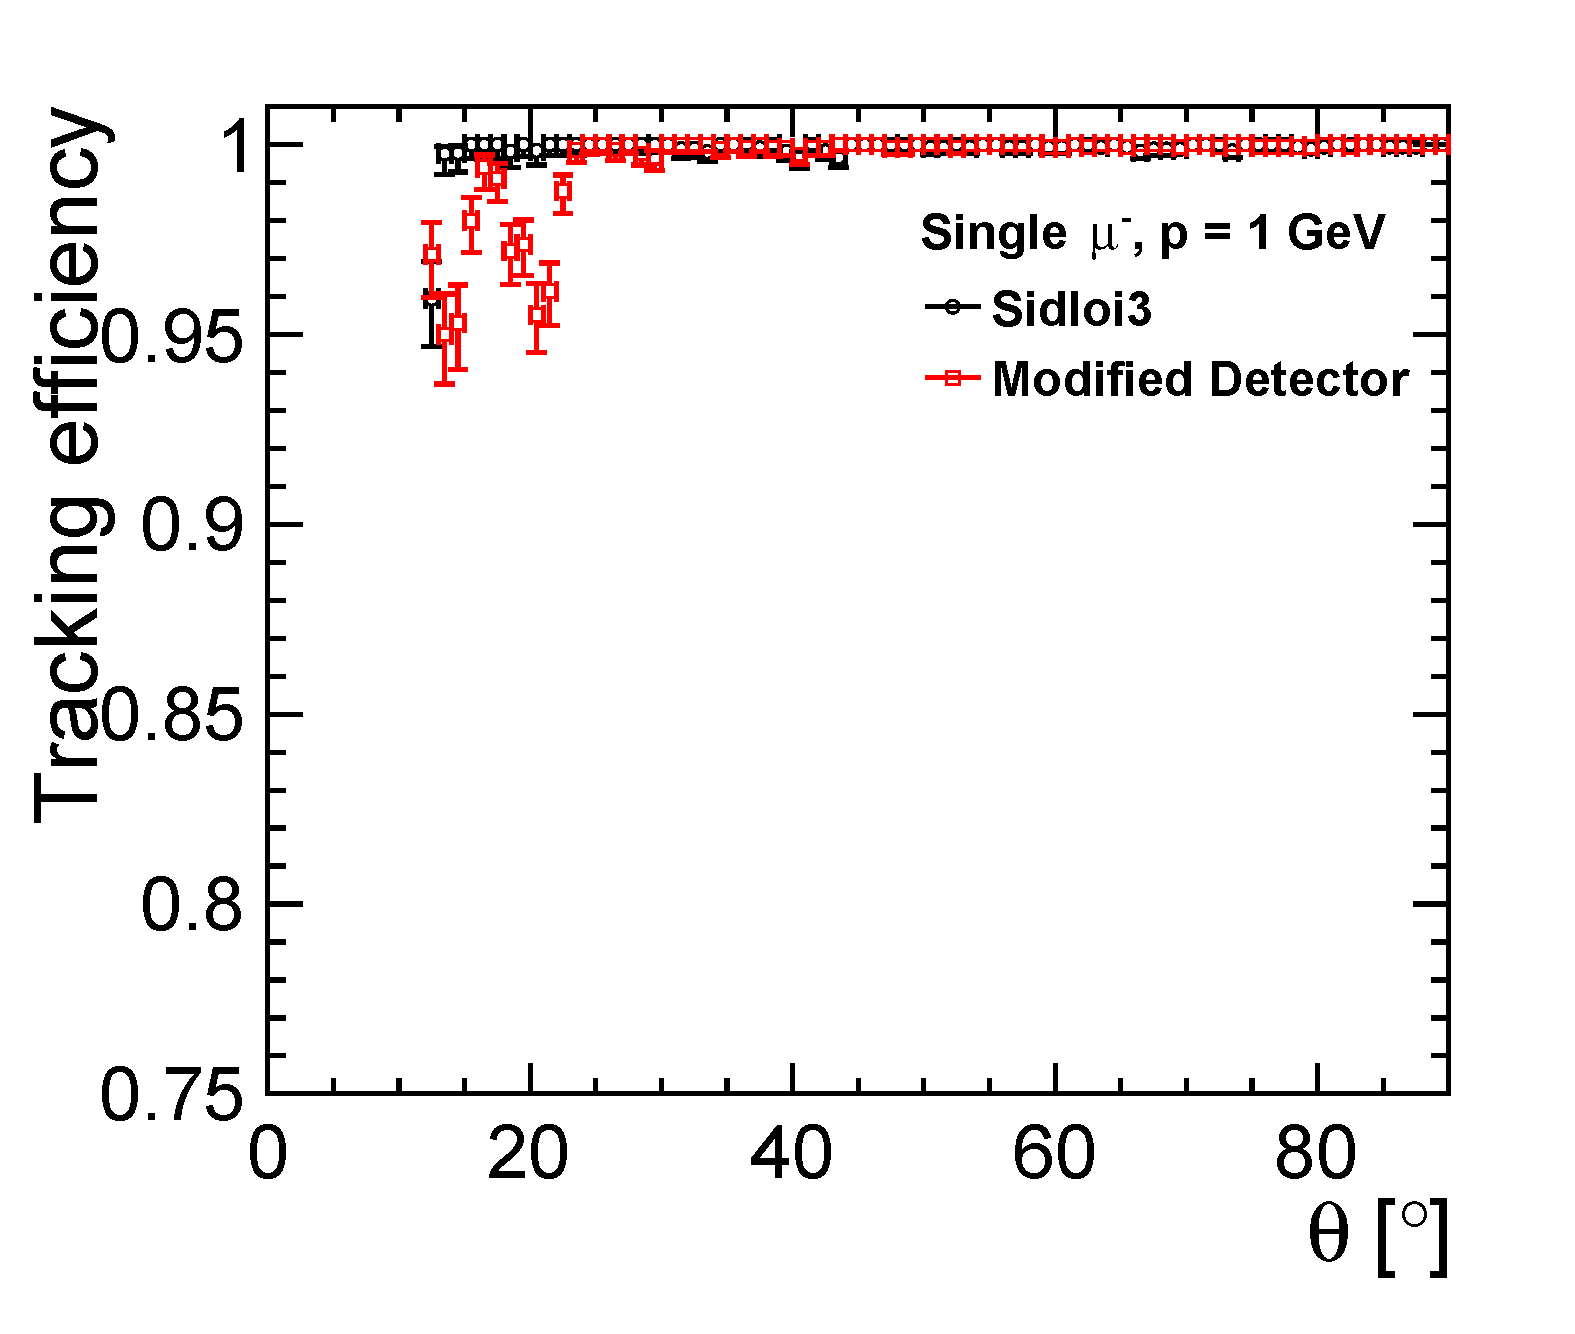
\includegraphics[width=2.0in]{muonEfficiencyThetaComparison1GeV.png}
\subcaption{$p$ = 1 GeV}\label{fig:muonefftheta1gev}
\end{minipage}%
\begin{minipage}{.33\textwidth}
\centering
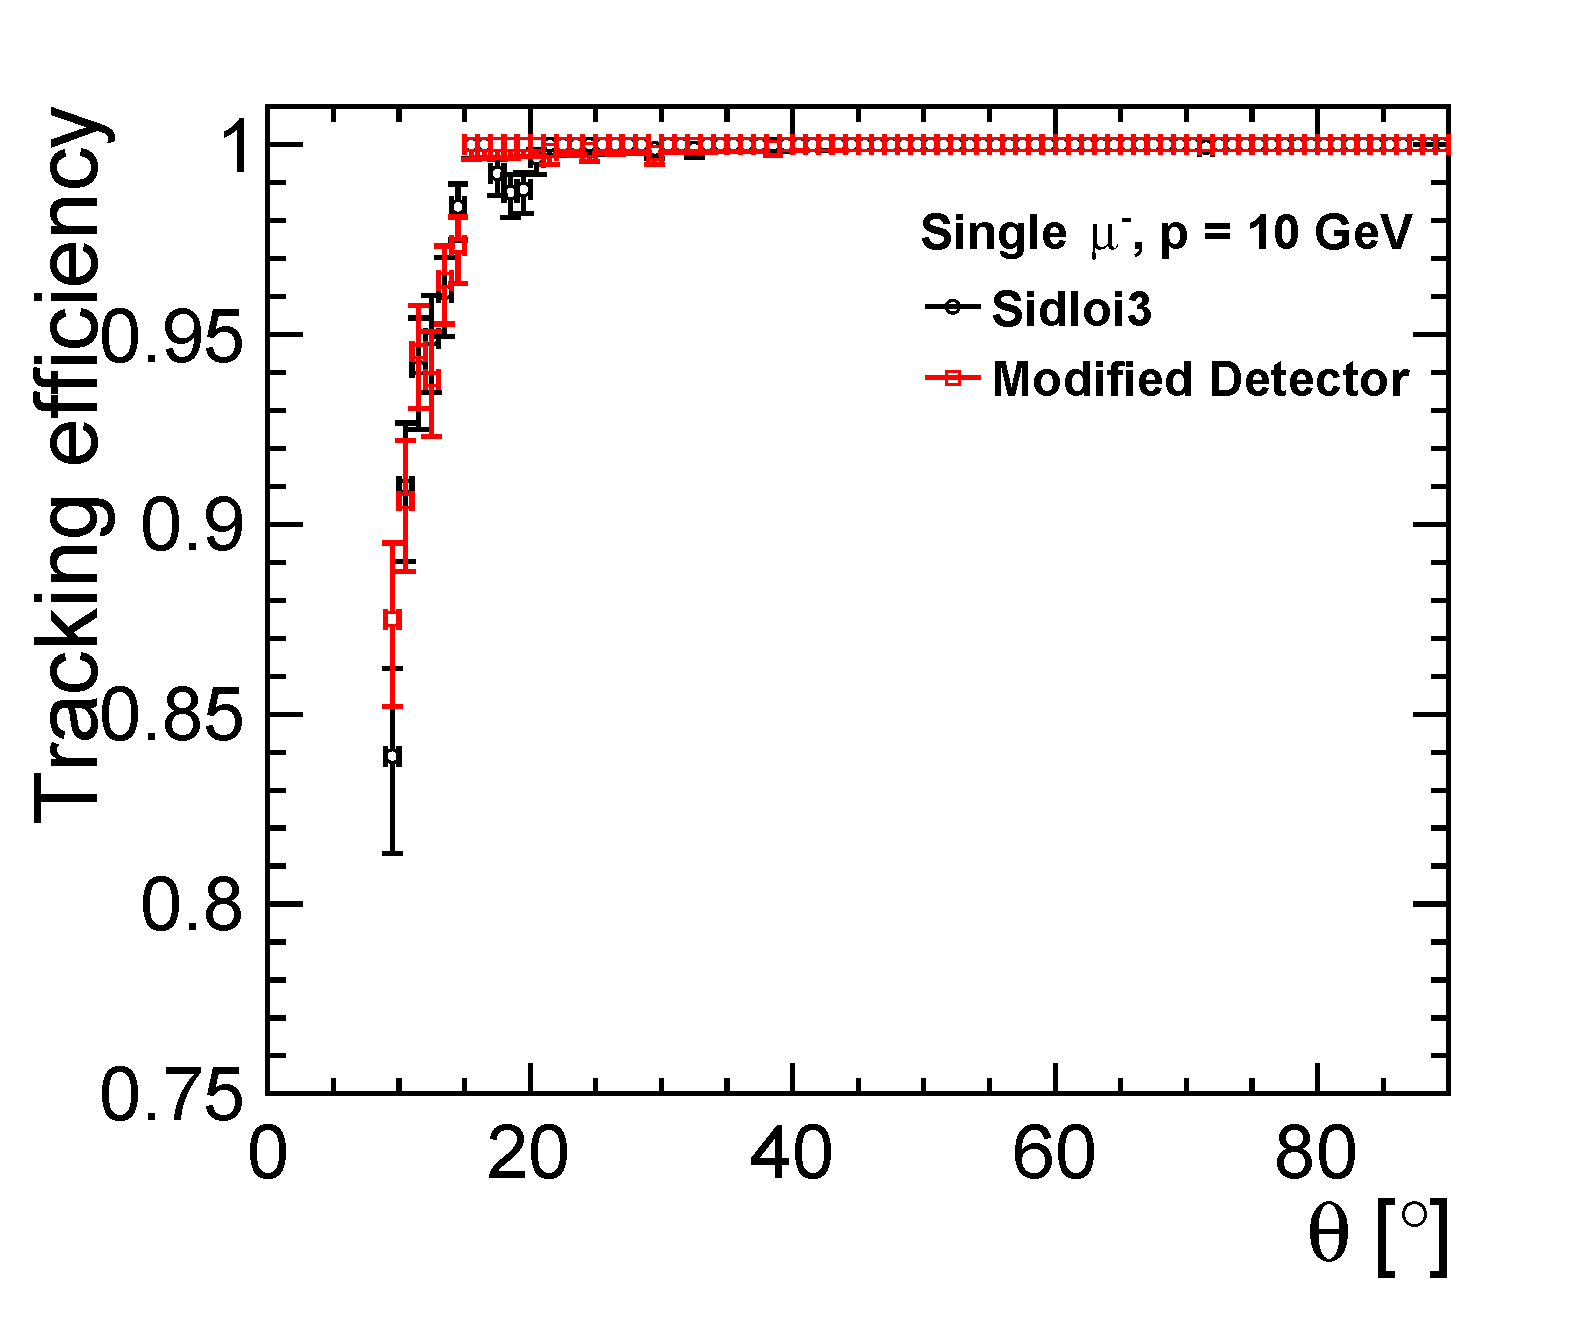
\includegraphics[width=2.0in]{muonEfficiencyThetaComparison10GeV.png}
\subcaption{$p$ = 10 GeV}\label{fig:muonefftheta10gev}
\end{minipage}
\begin{minipage}{.33\textwidth}
\centering
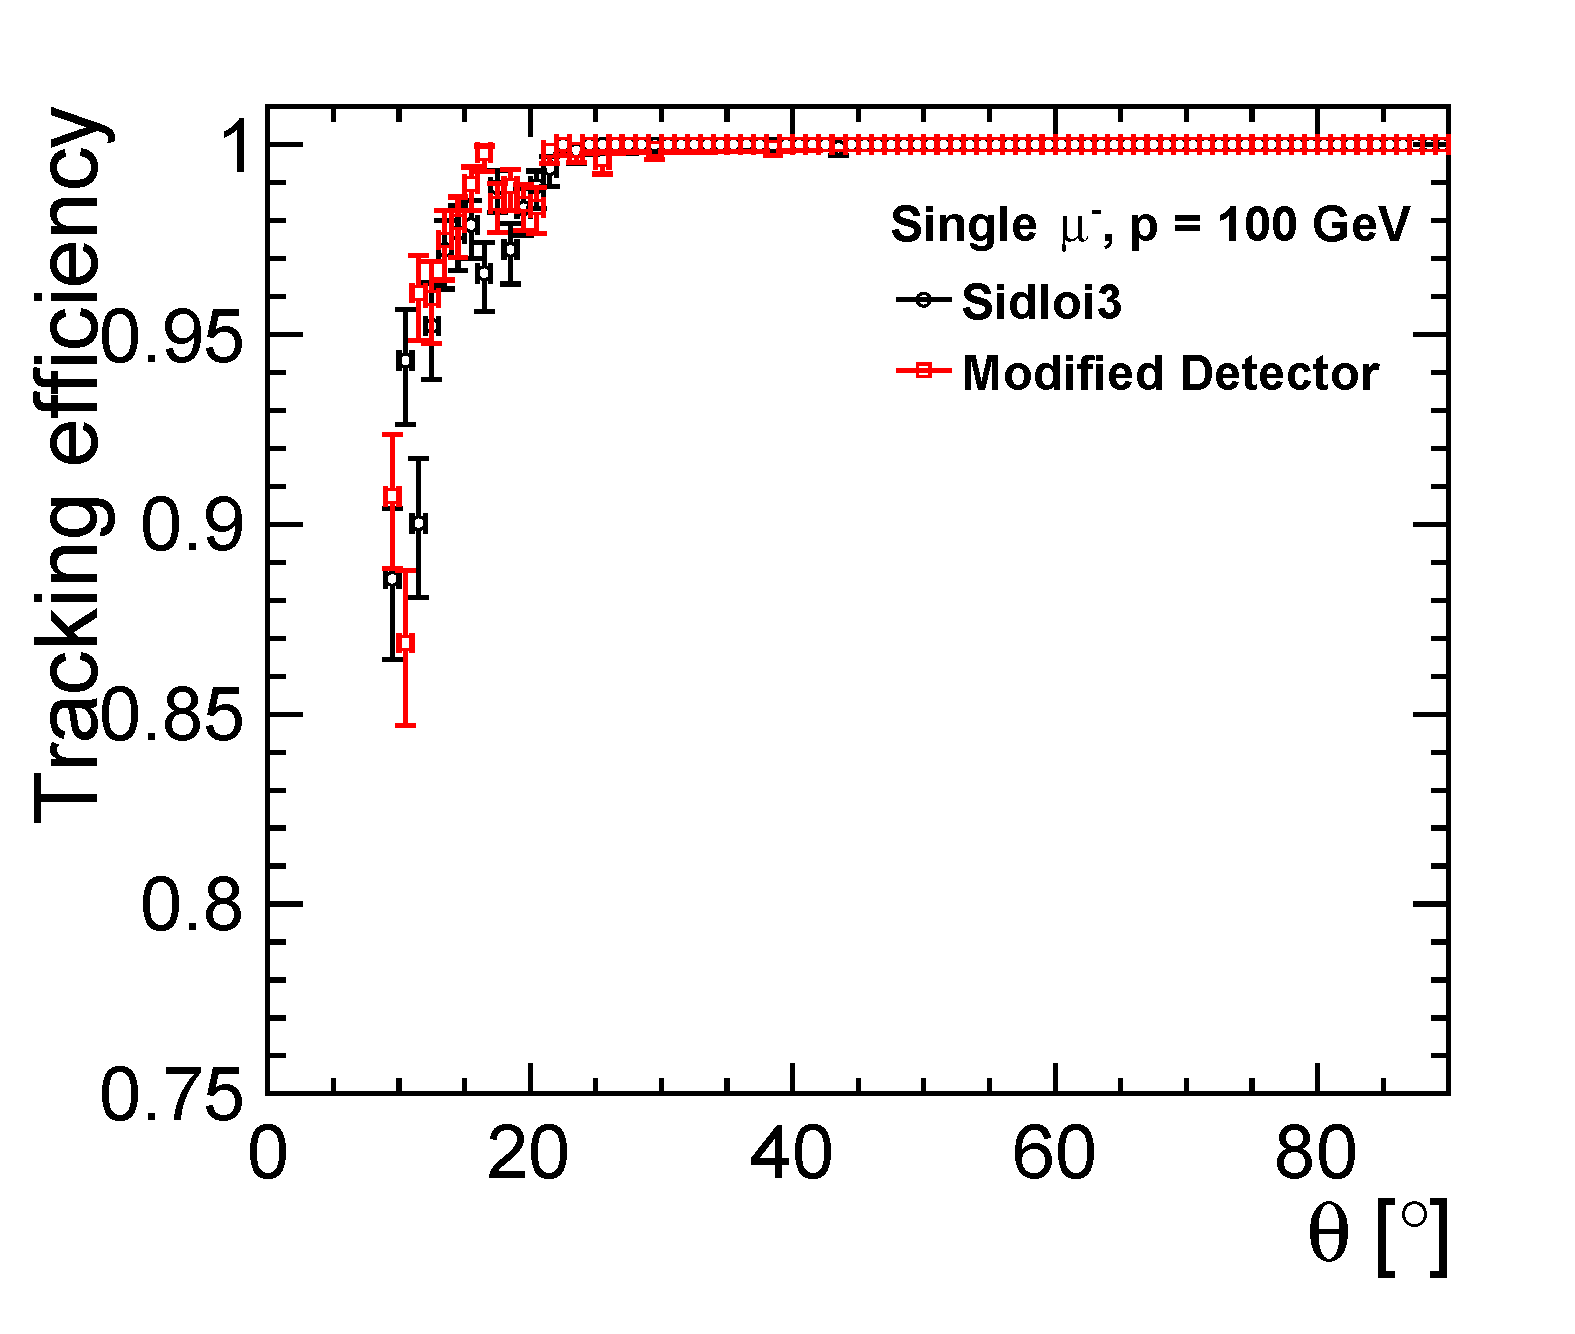
\includegraphics[width=2.0in]{muonEfficiencyThetaComparison100GeV.png}
\subcaption{$p$ = 100 GeV}\label{fig:muonefftheta100gev}
\end{minipage}
\caption{Tracking efficiency for single muons as a function of polar angle
for (a) 1 GeV, (b) 10 GeV, and (c) 100 GeV muons.}
\label{fig:muonefftheta}
\end{figure}

In figure~\ref{fig:muoneffpt}, the tracking efficiency has been plotted
with respect to the transverse momentum for various polar angles.
The difference in performance between the two detectors
%as illustrated with respect to polar angle (figure~\ref{fig:muonefftheta}) are 
is less clear.
Still, there is a slight dip in the modified detector's efficiency for low
transverse momentum muons ($p_{T} < 0.5$ GeV) at $\theta = 15^{\circ}$ (figure~\ref{fig:muoneffpt15theta})
and $\theta = 30^{\circ}$ (figure~\ref{fig:muoneffpt30theta}), echoing the results from figure~\ref{fig:muonefftheta1gev}.
Also, for $\theta = 90^{\circ}$ (figure~\ref{fig:muoneffpt90theta}), both detectors have idential performance for the full range of transverse momentum.
%which all three plots in figure~\ref{fig:muonefftheta} suggest.
%%% efficiency pt
\begin{figure}[h!]
\begin{minipage}{.33\textwidth}
\centering
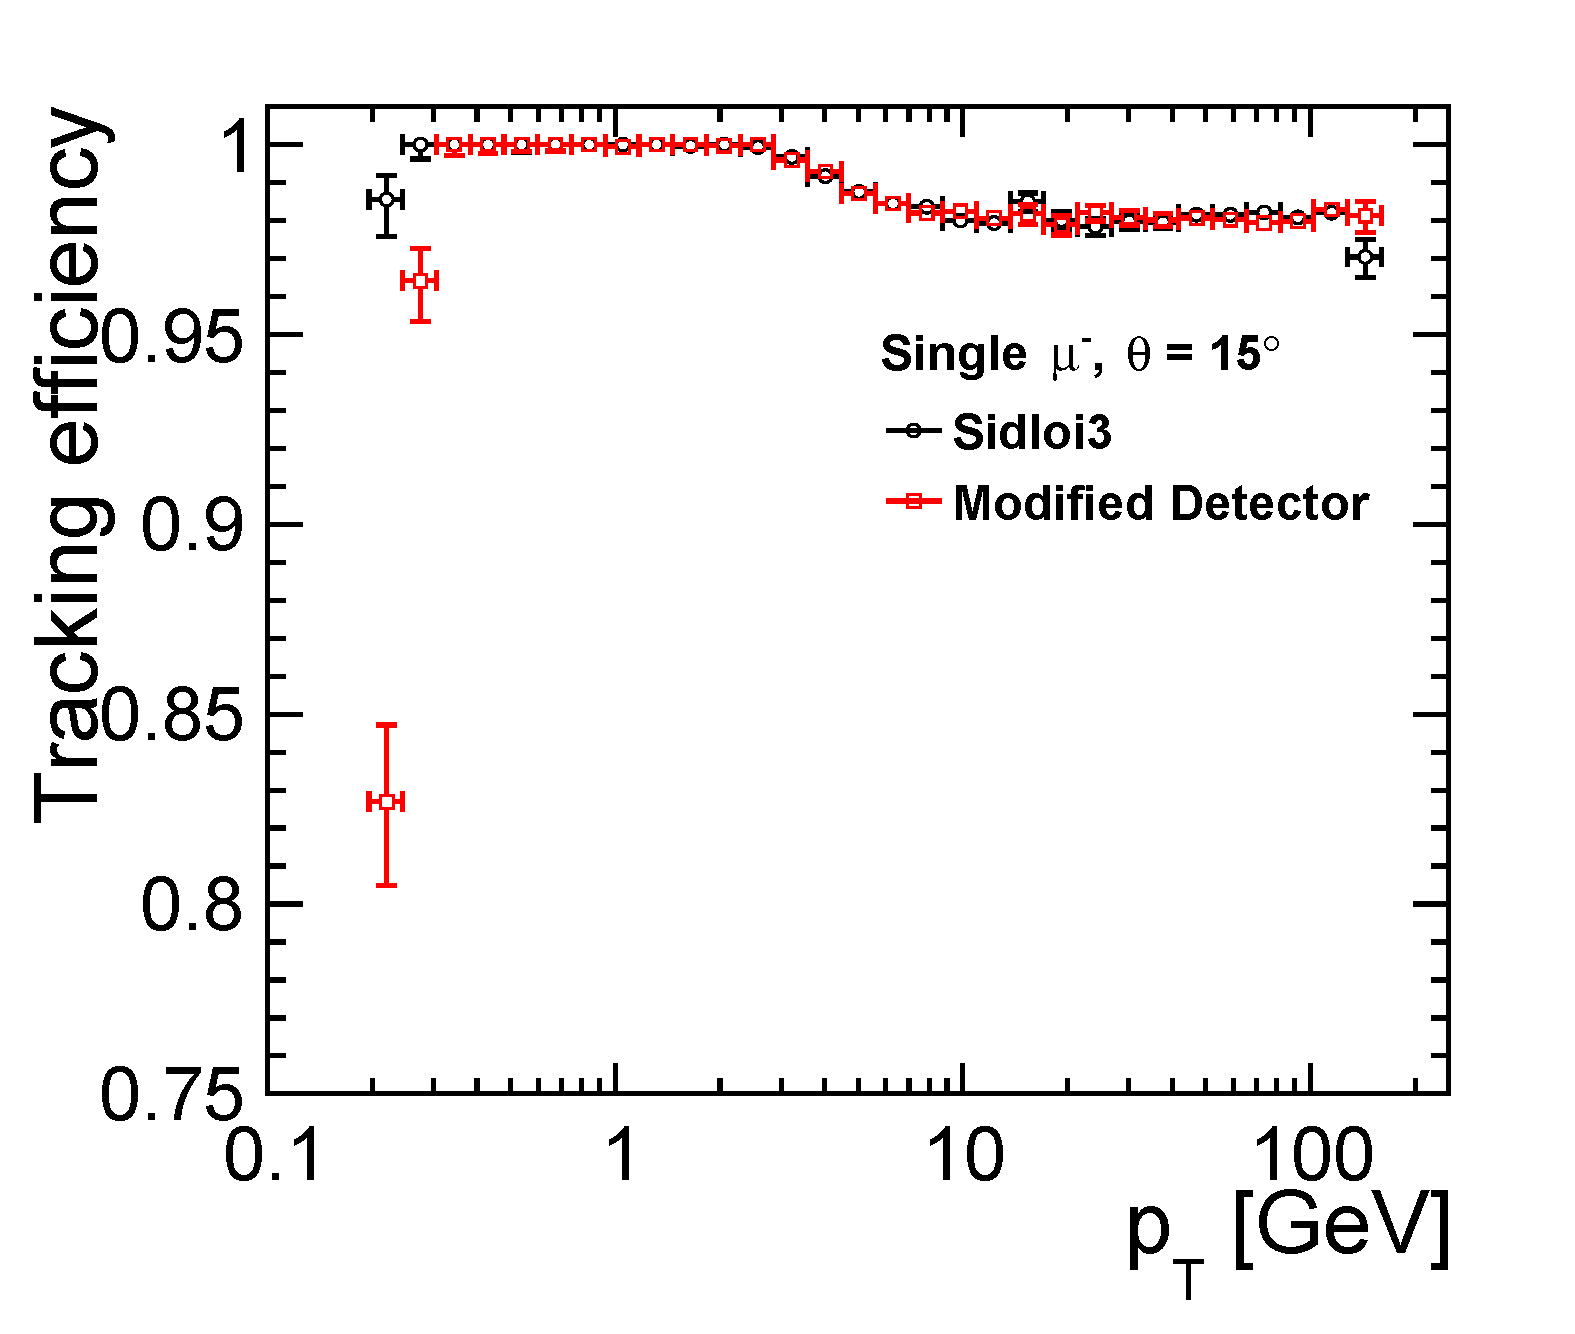
\includegraphics[width=2.0in]{muonEfficiencyPtComparisonTheta15.png}
\subcaption{$\theta = 15^{\circ}$}\label{fig:muoneffpt15theta}
\end{minipage}%
\begin{minipage}{.33\textwidth}
\centering
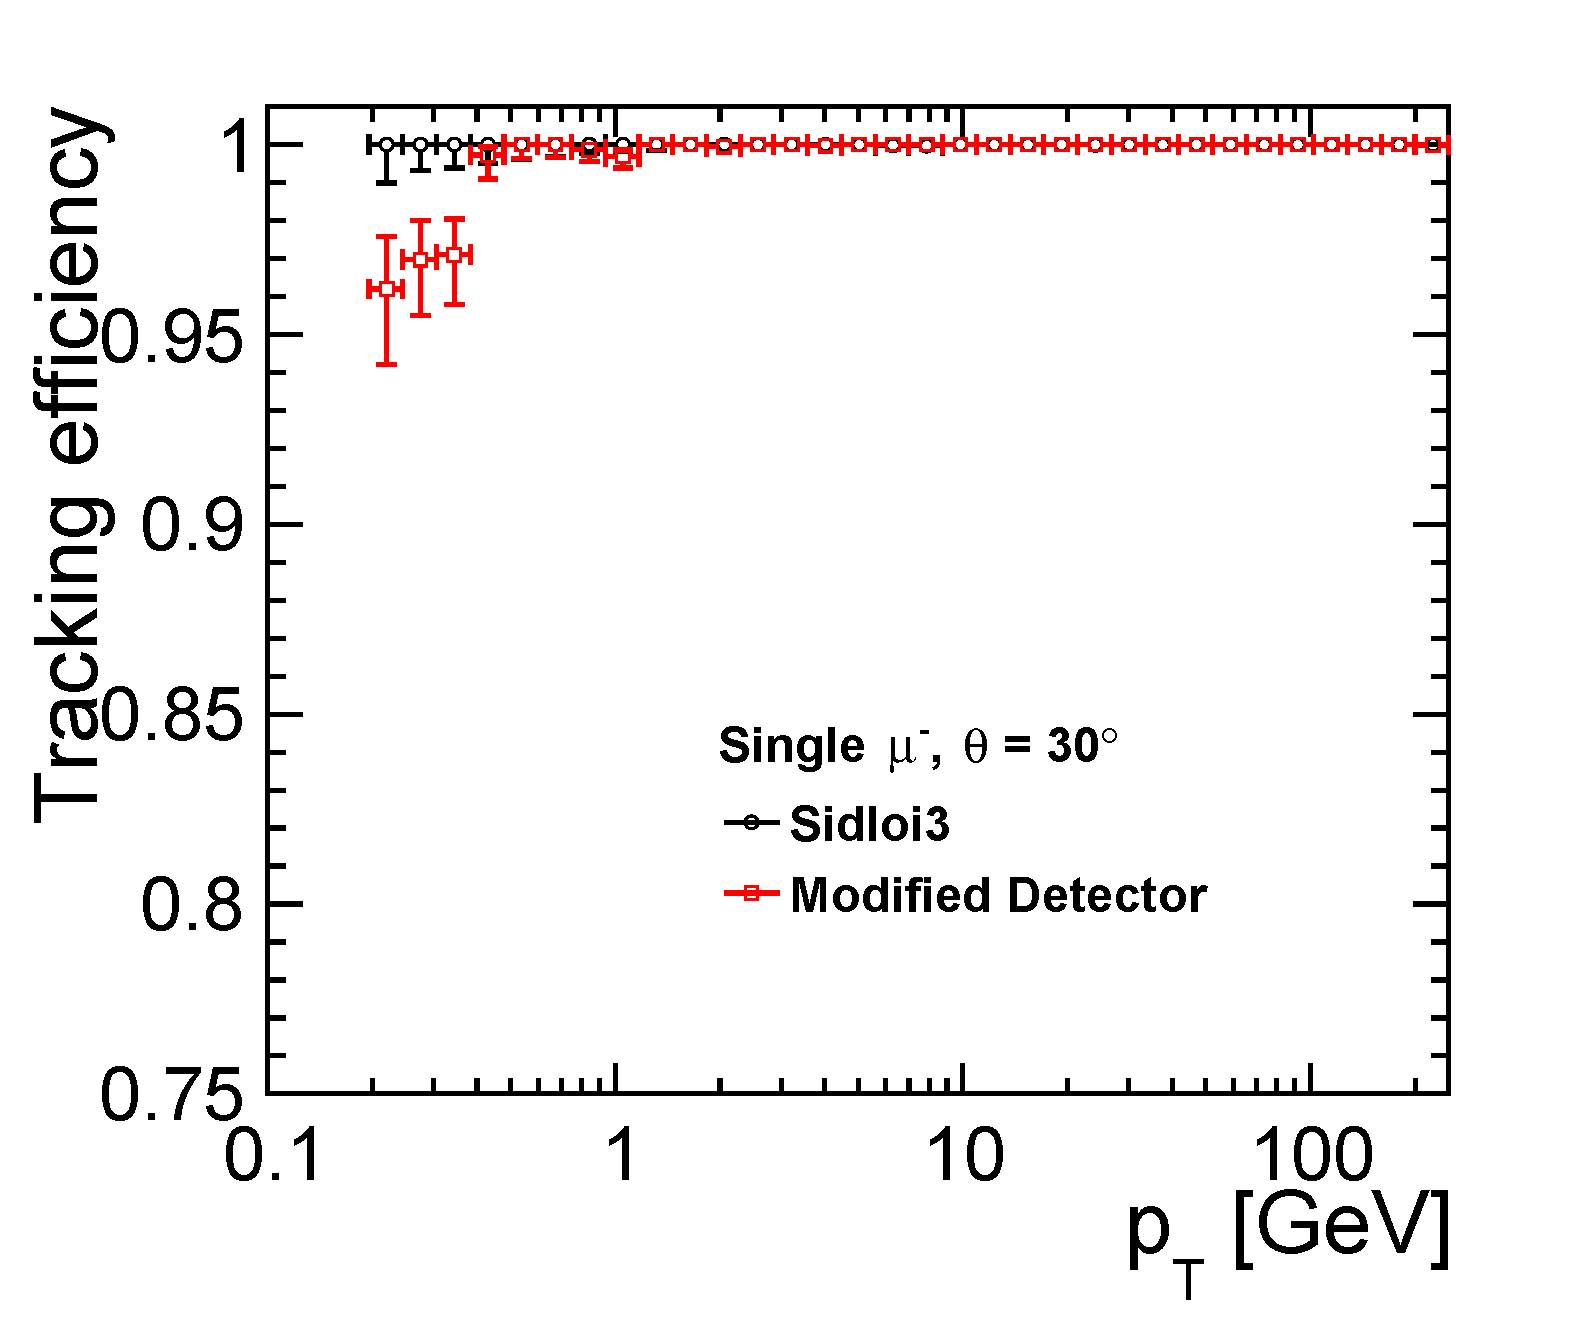
\includegraphics[width=2.0in]{muonEfficiencyPtComparisonTheta30.png}
\subcaption{$\theta = 30^{\circ}$}\label{fig:muoneffpt30theta}
\end{minipage}
\begin{minipage}{.33\textwidth}
\centering
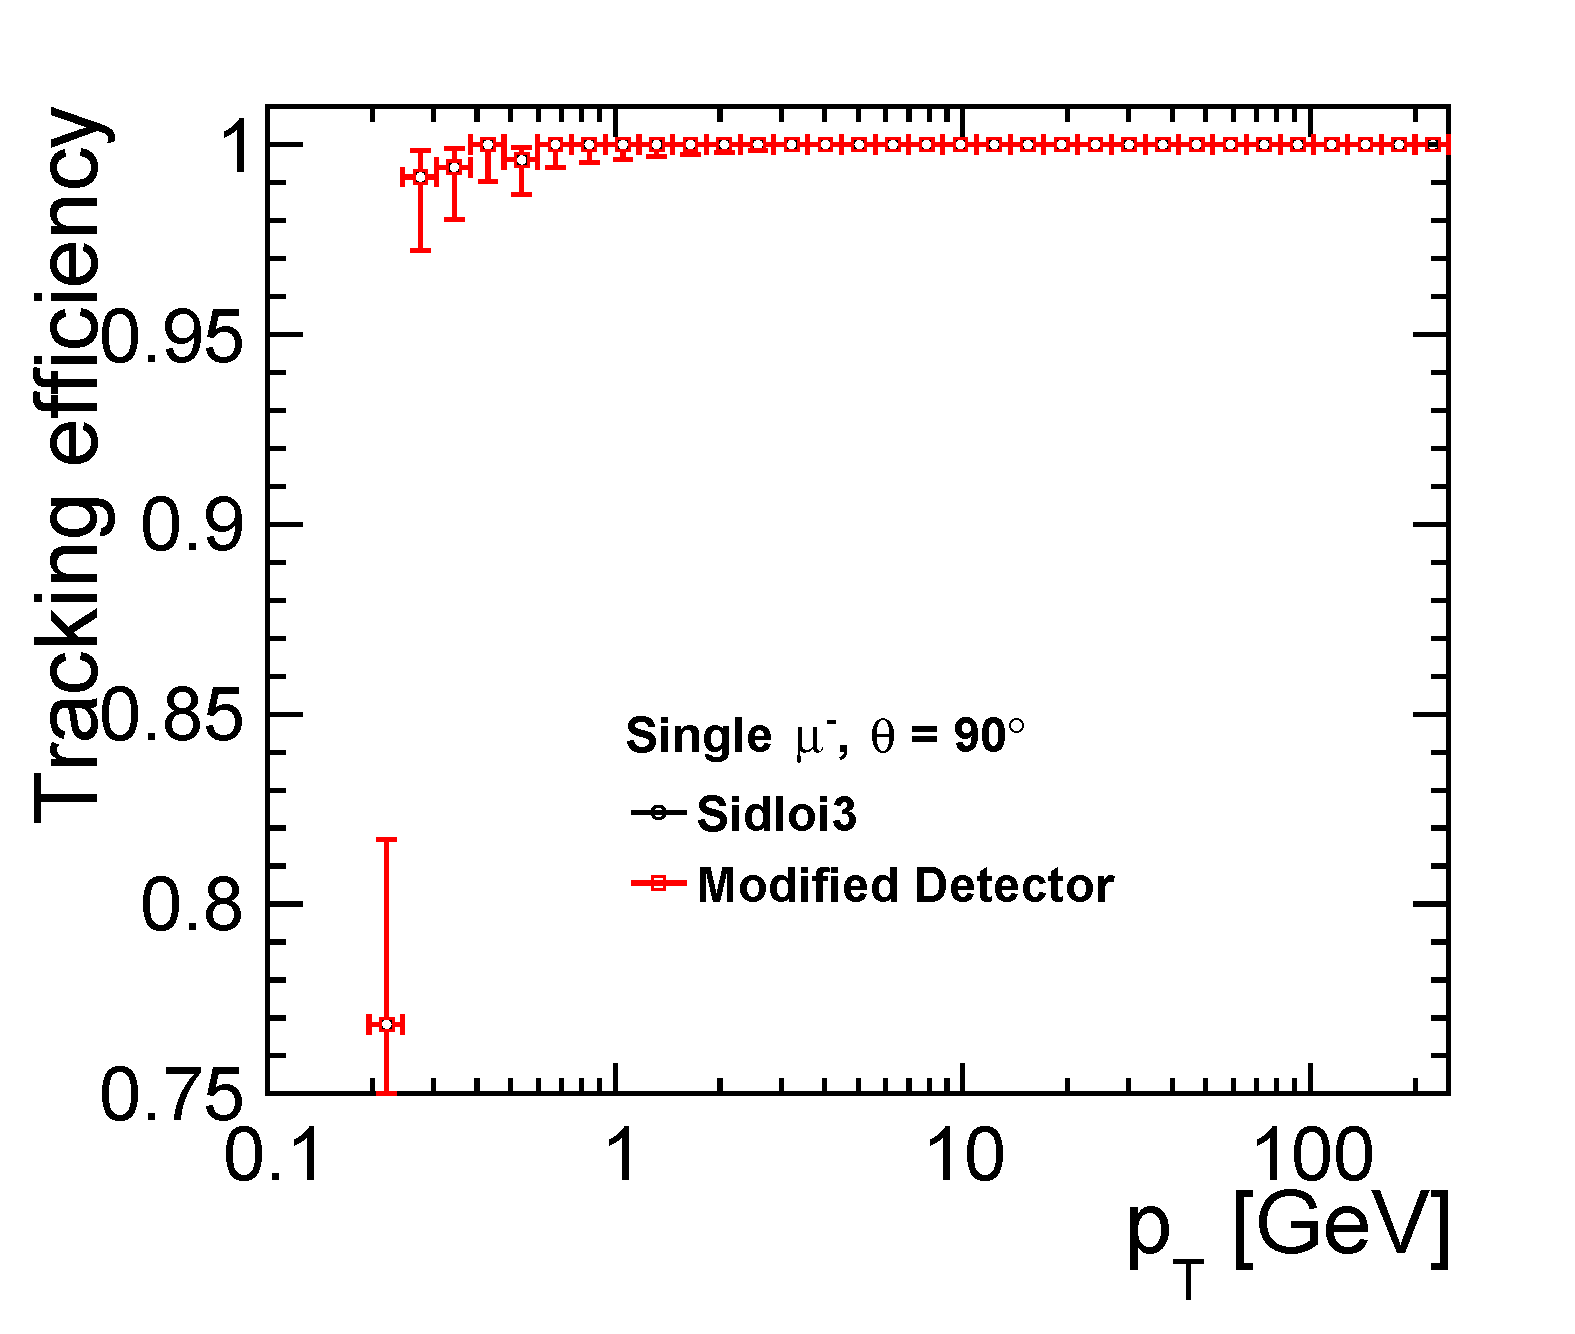
\includegraphics[width=2.0in]{muonEfficiencyPtComparisonTheta90.png}
\subcaption{$\theta = 90^{\circ}$}\label{fig:muoneffpt90theta}
\end{minipage}
\caption{Tracking efficiency for single muons as a function of transverse momentum
for muons at (a) $\theta = 15^{\circ}$, (b) $\theta = 30^{\circ}$, and (c) $\theta = 90^{\circ}$.}
\label{fig:muoneffpt}
\end{figure}

\subsubsection{$\ee \rightarrow \ttbar$, $ \sqrt{s} = $ 500 GeV}
For $\ee \rightarrow \ttbar$ events, the modified detector demonstrated greater efficiency than Sidloi3 for lower transverse
momentum particles (0.5 GeV $< p_{T} < $ 30 GeV) for $\theta > 30^{\circ}$,
as illustrated in figure~\ref{fig:eettbareffthetalowpt} and figure~\ref{fig:eettbareffthetamedpt}.
On the other hand, as shown in figure~\ref{fig:eettbareffthetahighpt}, the modified detector  
had slightly worse efficiency than Sidloi3 for
higher transverse momentum particles (30 GeV $< p_{T} $) at $\theta > 60^{\circ}$.
The distinction between both detectors blurs for low polar angles ($\theta < 30^{\circ}$).
%with the performance of both detectors comparable.
%%%efficiency theta
\begin{figure}[h!]
\begin{minipage}{.33\textwidth}
\centering
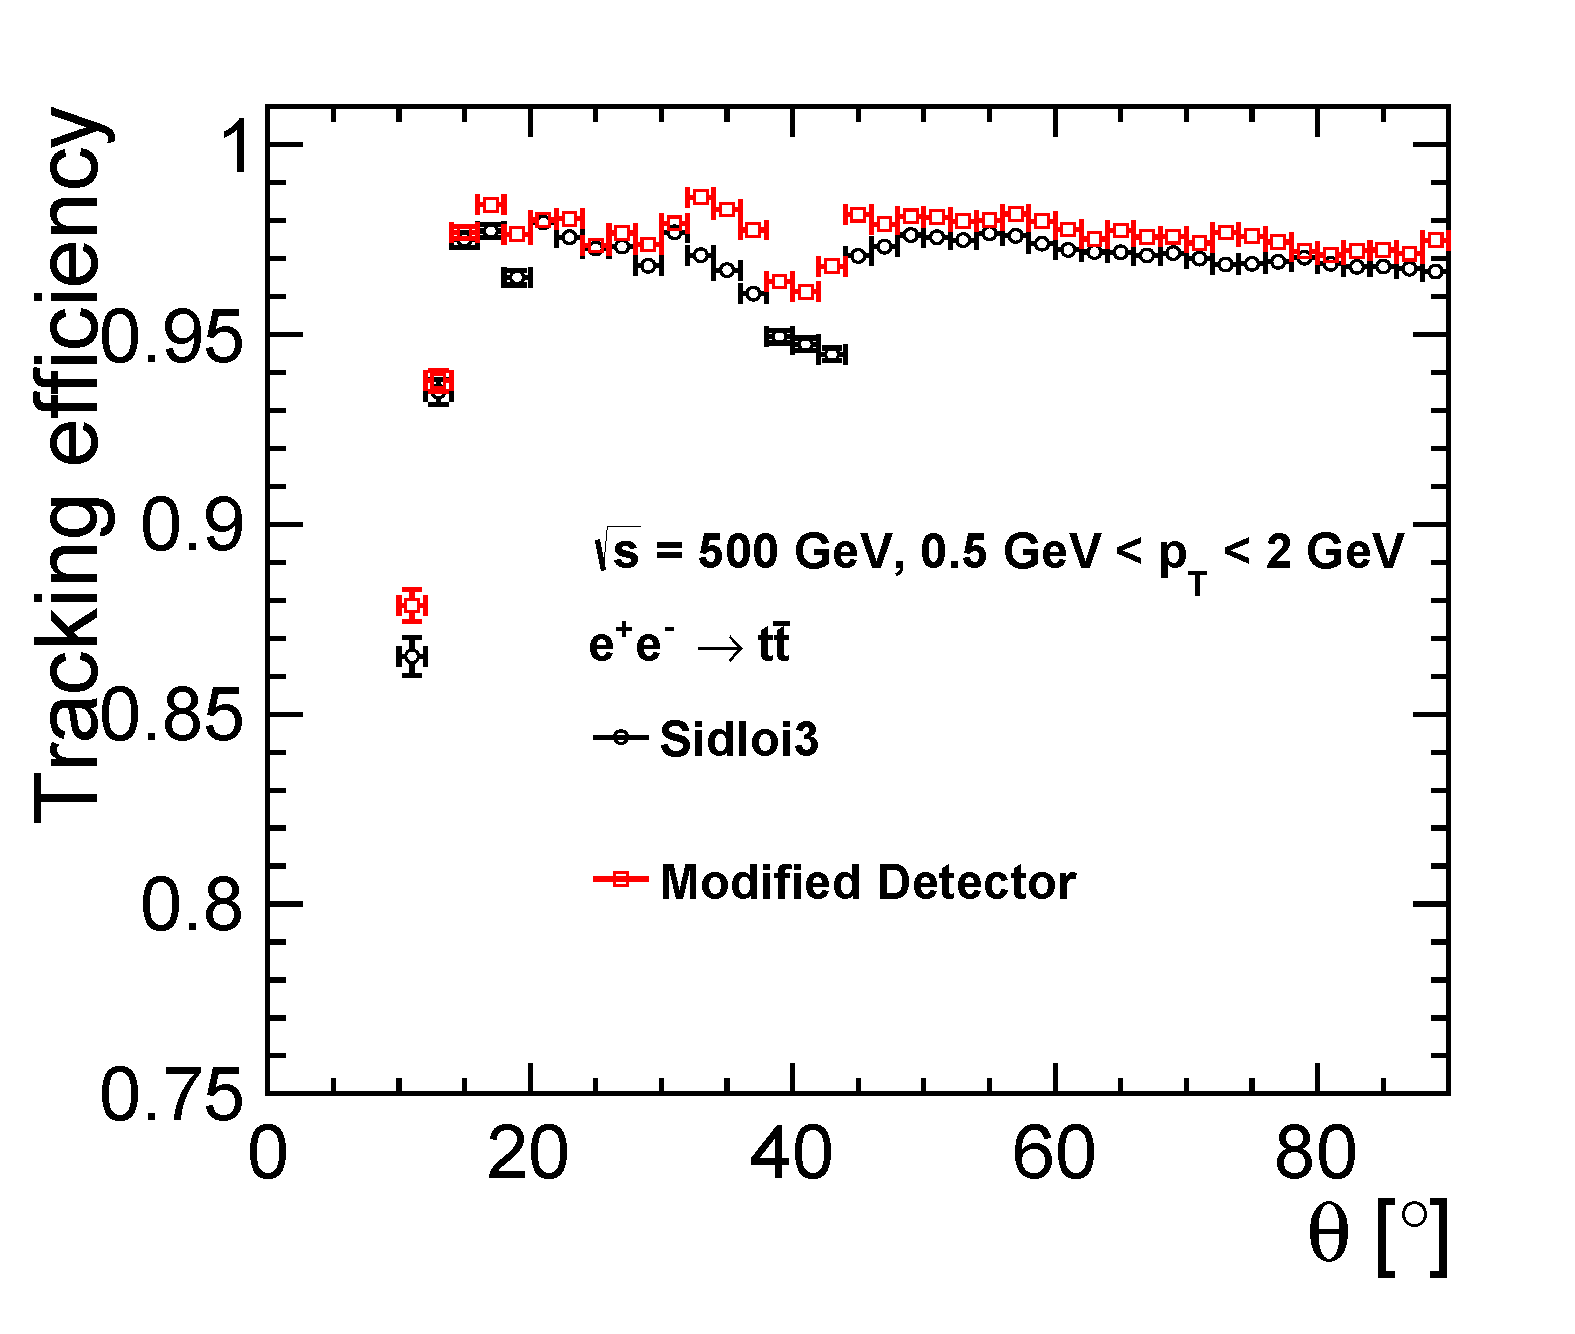
\includegraphics[width=2.0in]{eettbarEfficiencyThetaLowPt_sidloi3_det_vtxbar_3doublet.png}
\subcaption{0.5 GeV $< p_{T} < $ 2 GeV}\label{fig:eettbareffthetalowpt}
\end{minipage}%
\begin{minipage}{.33\textwidth}
\centering
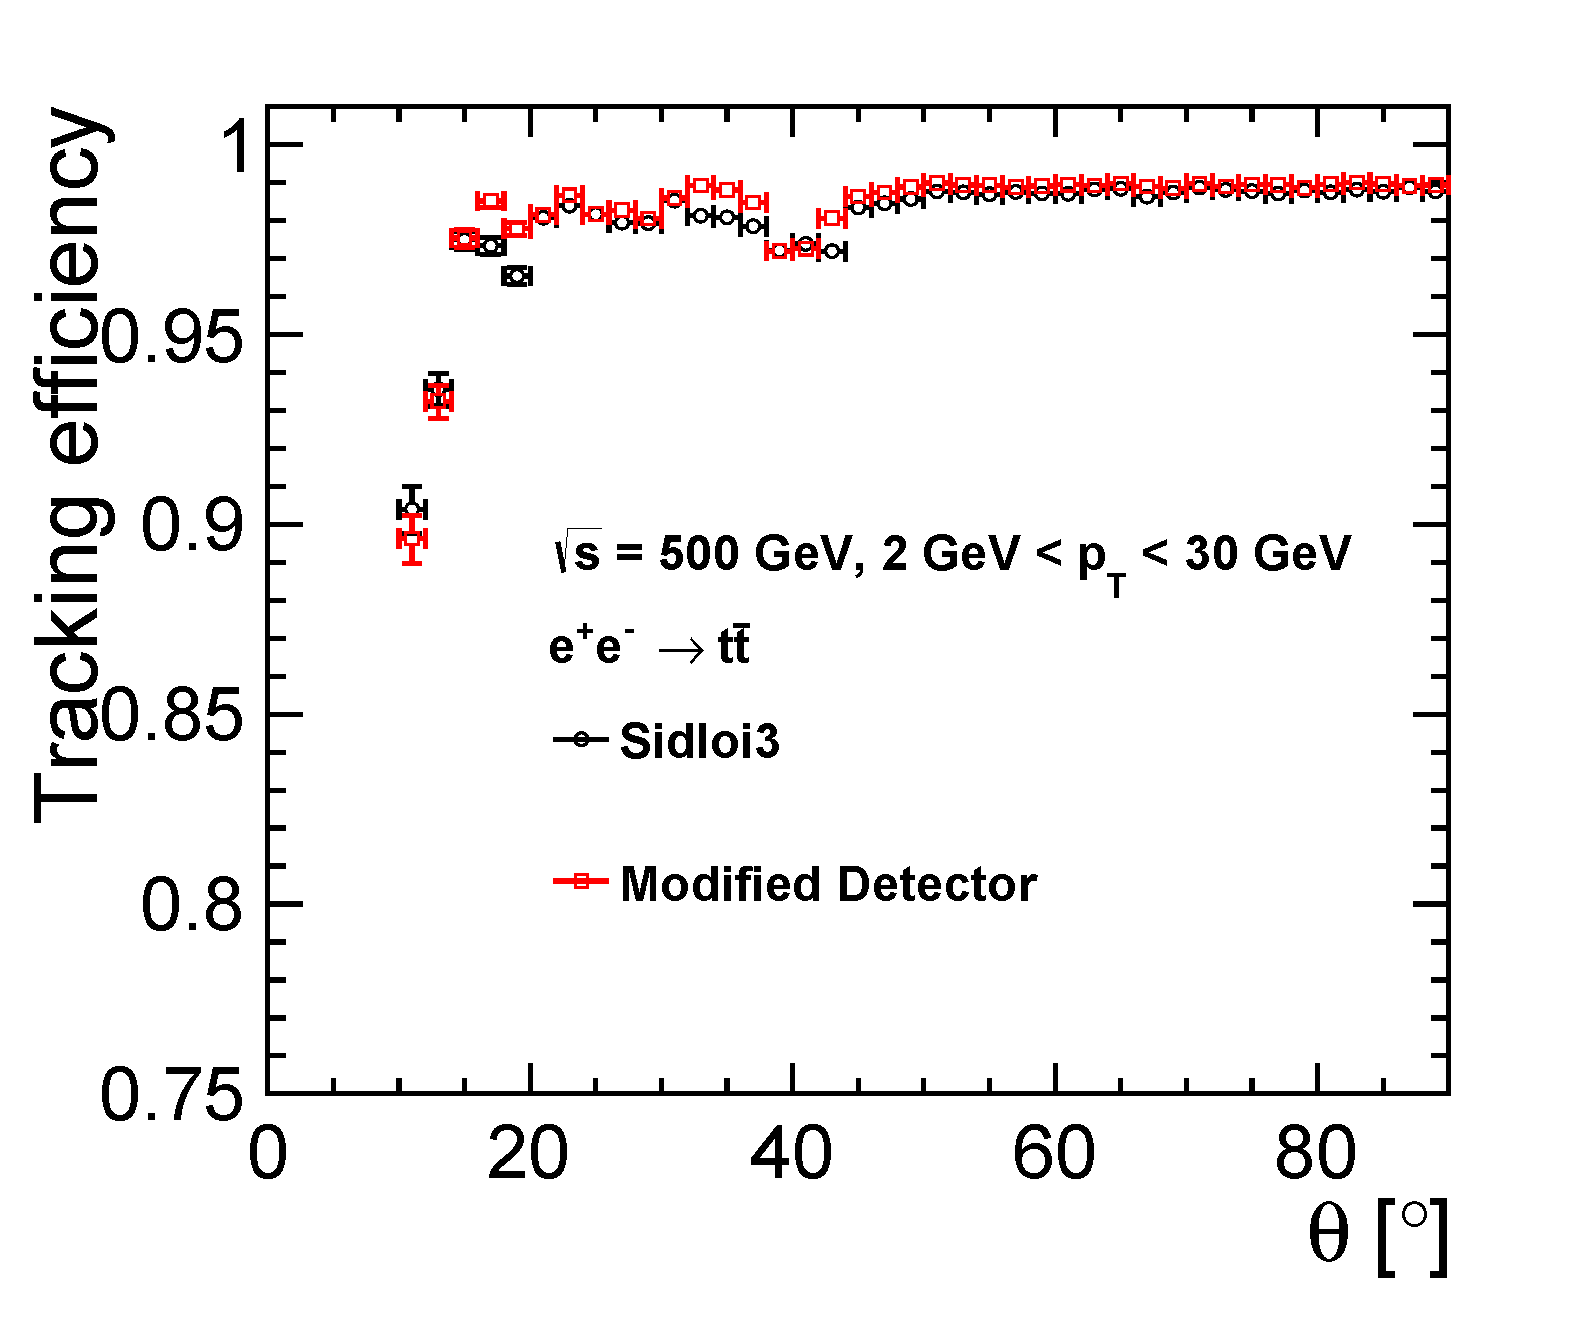
\includegraphics[width=2.0in]{eettbarEfficiencyThetaMedPt_sidloi3_det_vtxbar_3doublet.png}
\subcaption{2 GeV $< p_{T} < $ 30 GeV}\label{fig:eettbareffthetamedpt}
\end{minipage}
\begin{minipage}{.33\textwidth}
\centering
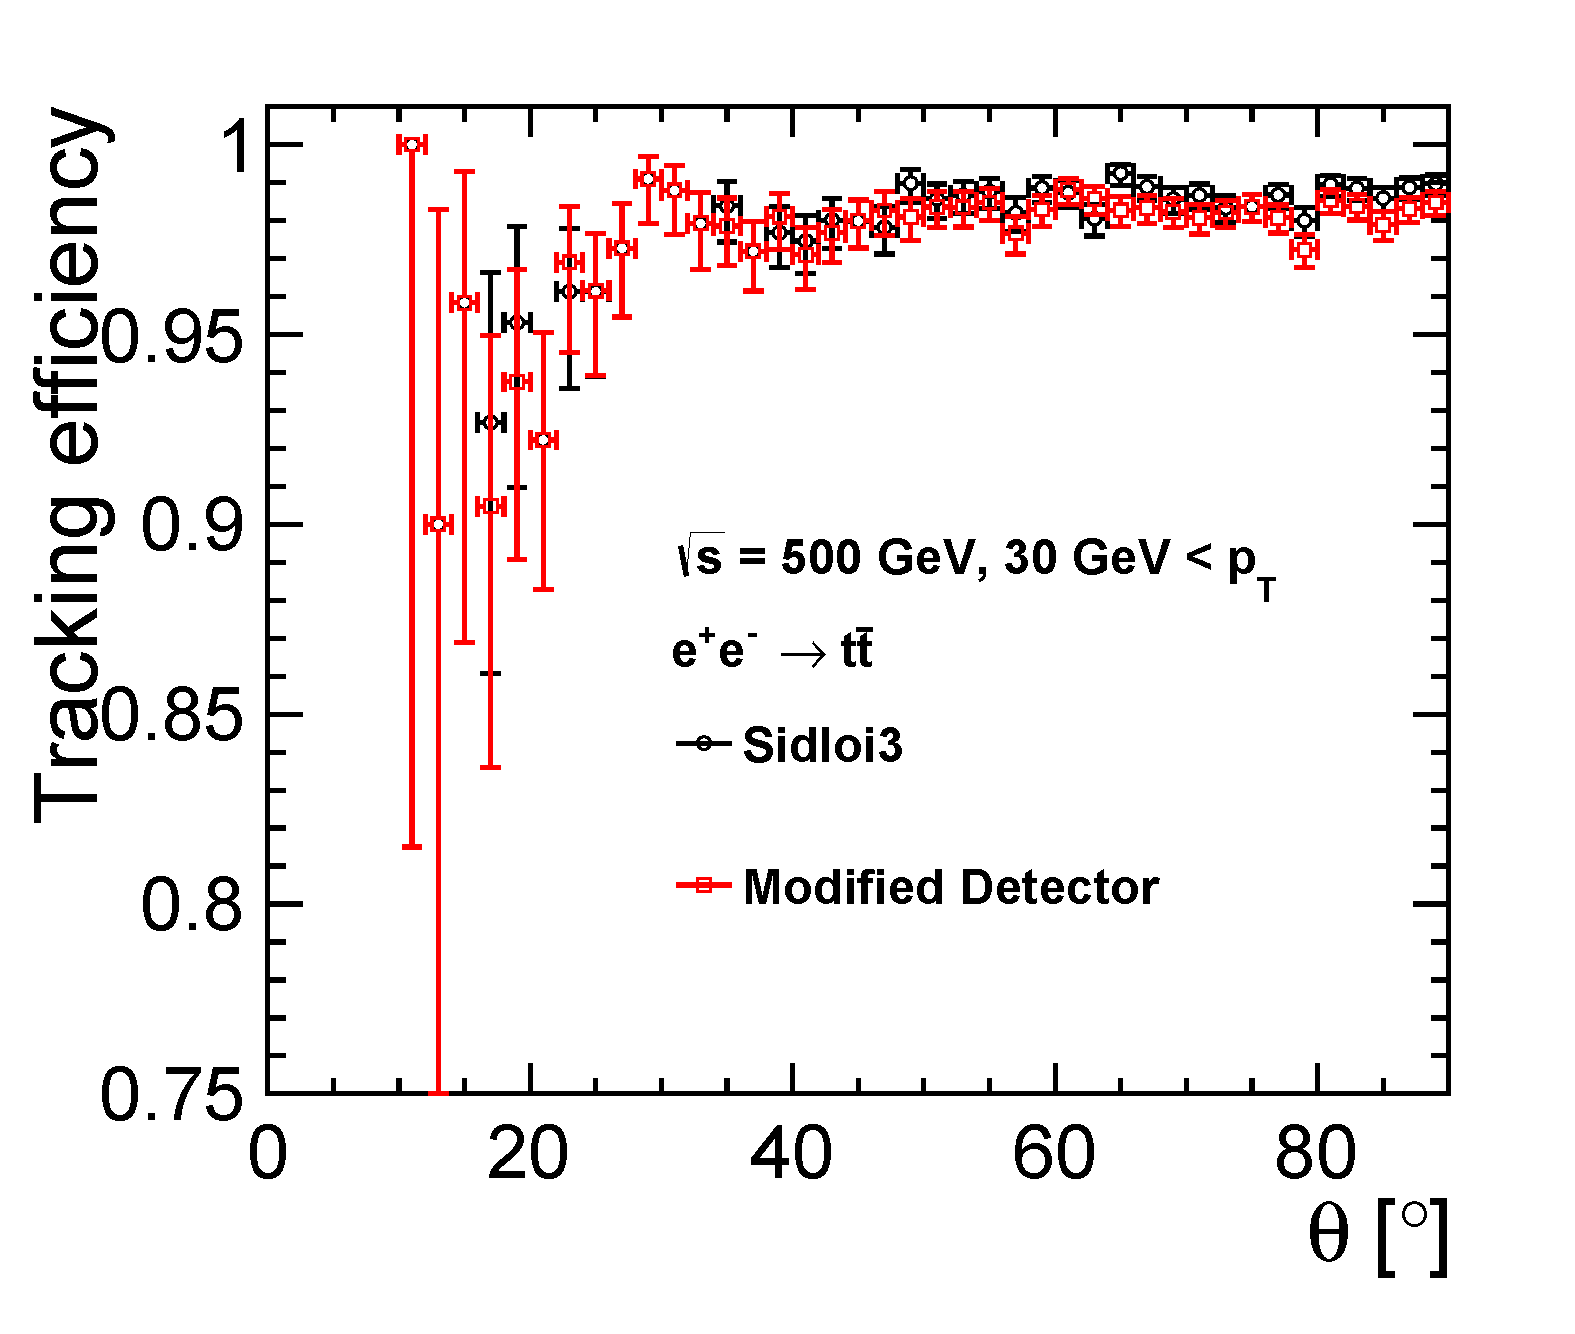
\includegraphics[width=2.0in]{eettbarEfficiencyTheta30GeV_sidloi3_det_vtxbar_3doublet.png}
\subcaption{30 GeV $< p_{T} $}\label{fig:eettbareffthetahighpt}
\end{minipage}
\caption{Tracking efficiency for $\ee \rightarrow \ttbar$ at $ \sqrt{s} = $ 500 GeV as a function of polar angle
for (a) 0.5 GeV $< p_{T} < $ 2 GeV, (b) 2 GeV $< p_{T} < $ 30 GeV, and (c) 30 GeV $< p_{T} $ particles.}
\label{fig:eettbarefftheta}
\end{figure}

Similarly, when efficiency is plotted versus transverse momentum (figure~\ref{fig:eettbareffpt}), the modified detector
exhibits greater efficiency for lower transverse momentum particles (0.5 GeV $< p_{T} <$ 10 GeV) at low polar angle ($10^{\circ} < \theta$).
This is evident in all three plots in figure~\ref{fig:eettbareffpt}
 (figures~\ref{fig:eettbareffptlowtheta},~\ref{fig:eettbareffptmedtheta},~\ref{fig:eettbareffpthightheta}).
However, as shown in figure~\ref{fig:eettbareffpthightheta}, 
for greater polar angles ($45^{\circ} < \theta$), once particles have transverse momentum $p_{T} > $ 20 GeV,
Sidloi3 performs better, mirroring the performance as shown in figure~\ref{fig:eettbareffthetahighpt}.
For particles with 1 GeV $< p_{T}<$ 20 GeV, both detectors perform
similarly well for polar angles  ($\theta > 10^{\circ}$), evident in all three plots in figure~\ref{fig:eettbareffpt}.
%%%efficiency pt
\begin{figure}[h!]
\begin{minipage}{.33\textwidth}
\centering
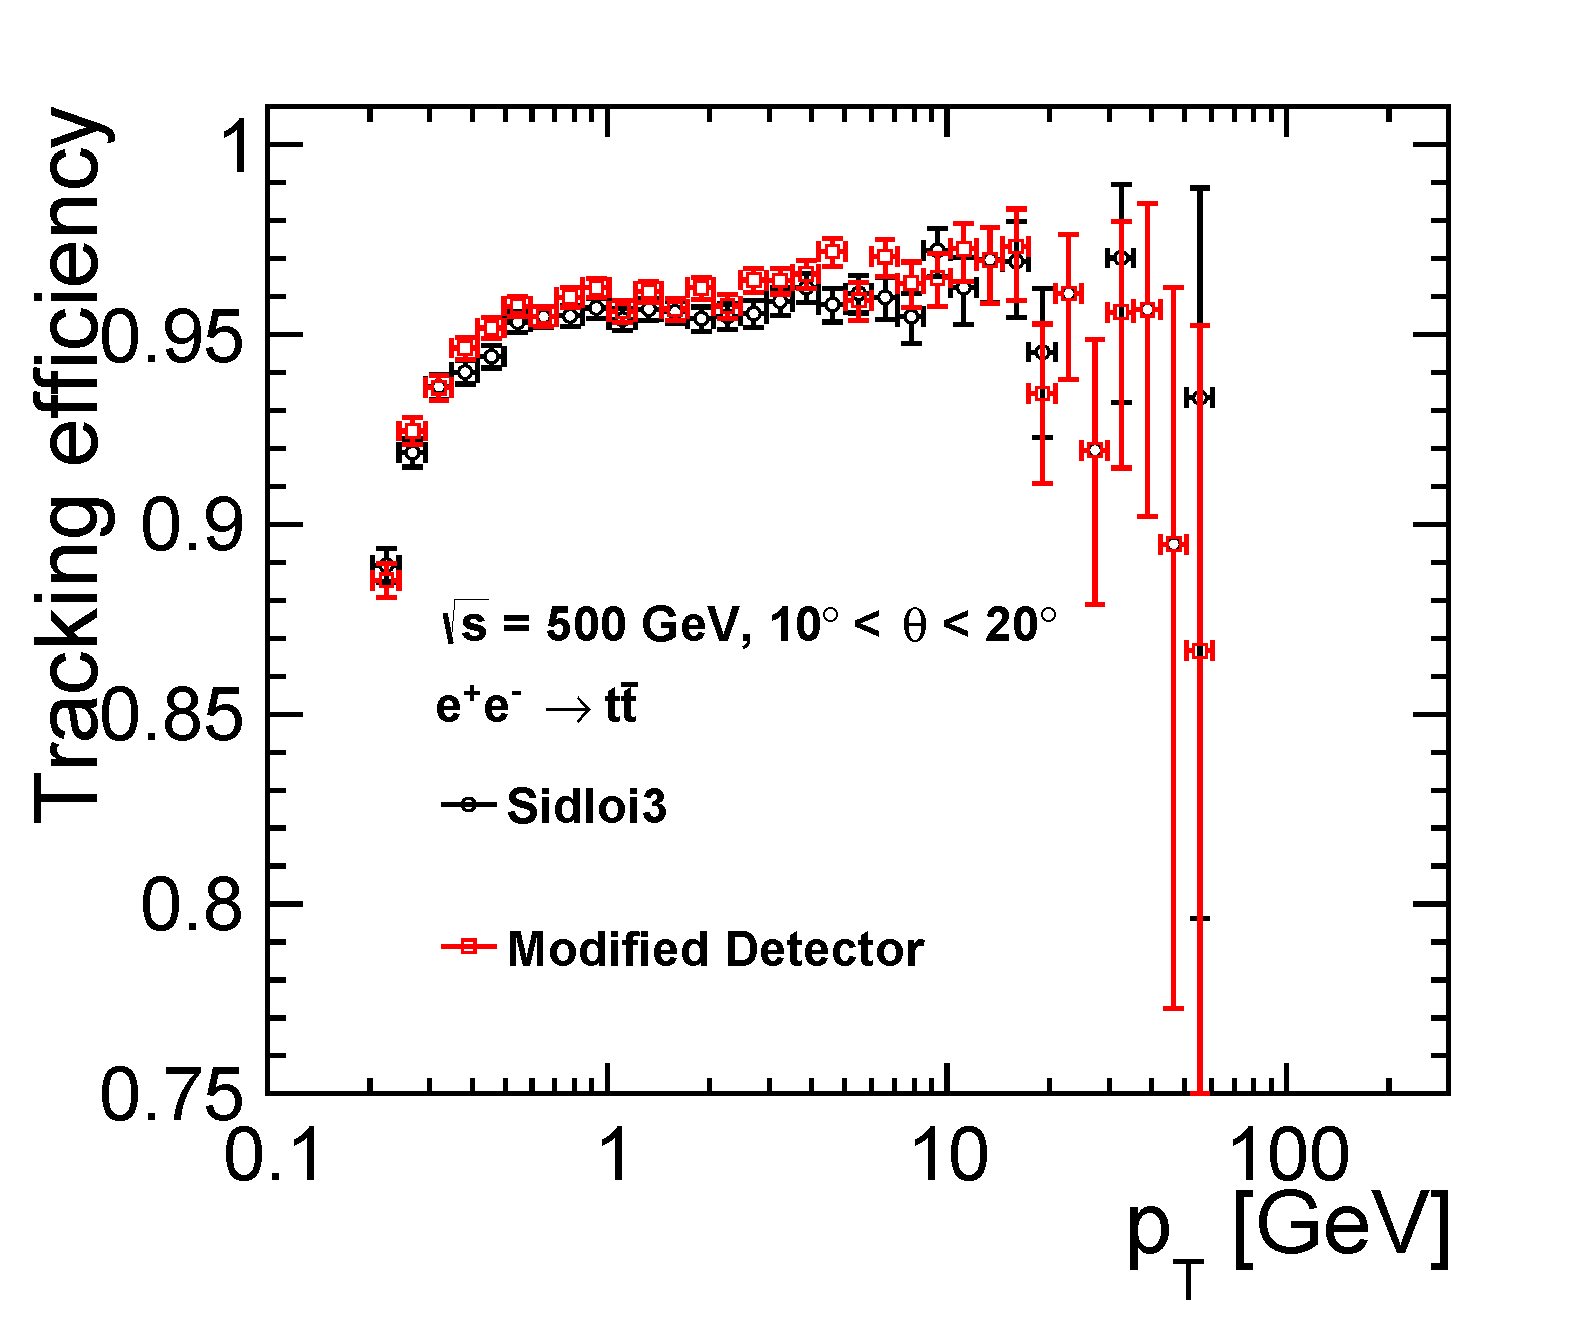
\includegraphics[width=2.0in]{eettbarEfficiencyPtLowTheta_sidloi3_det_vtxbar_3doublet.png}
\subcaption{$10^{\circ}< \theta <  20^{\circ}$}\label{fig:eettbareffptlowtheta}
\end{minipage}%
\begin{minipage}{.33\textwidth}
\centering
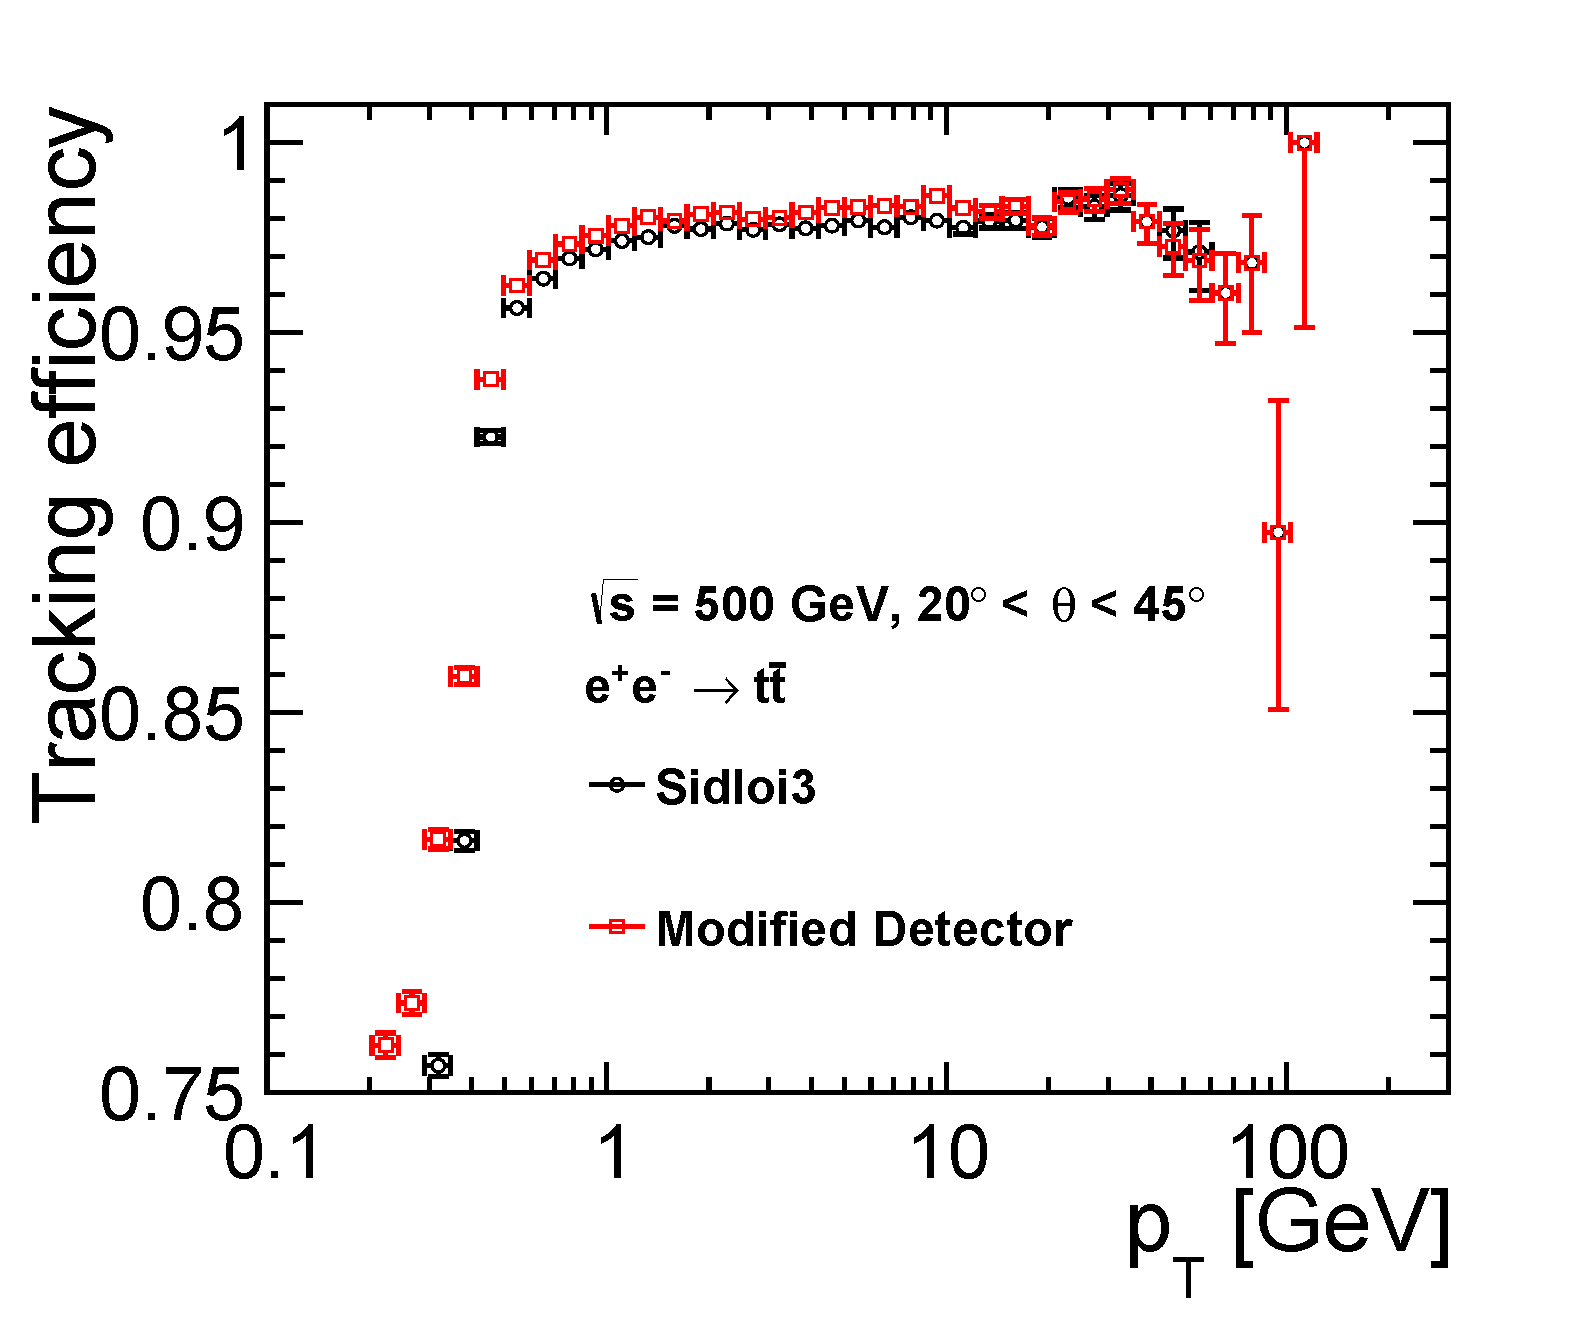
\includegraphics[width=2.0in]{eettbarEfficiencyPtMedTheta_sidloi3_det_vtxbar_3doublet.png}
\subcaption{$20^{\circ}< \theta <  45^{\circ}$}\label{fig:eettbareffptmedtheta}
\end{minipage}
\begin{minipage}{.33\textwidth}
\centering
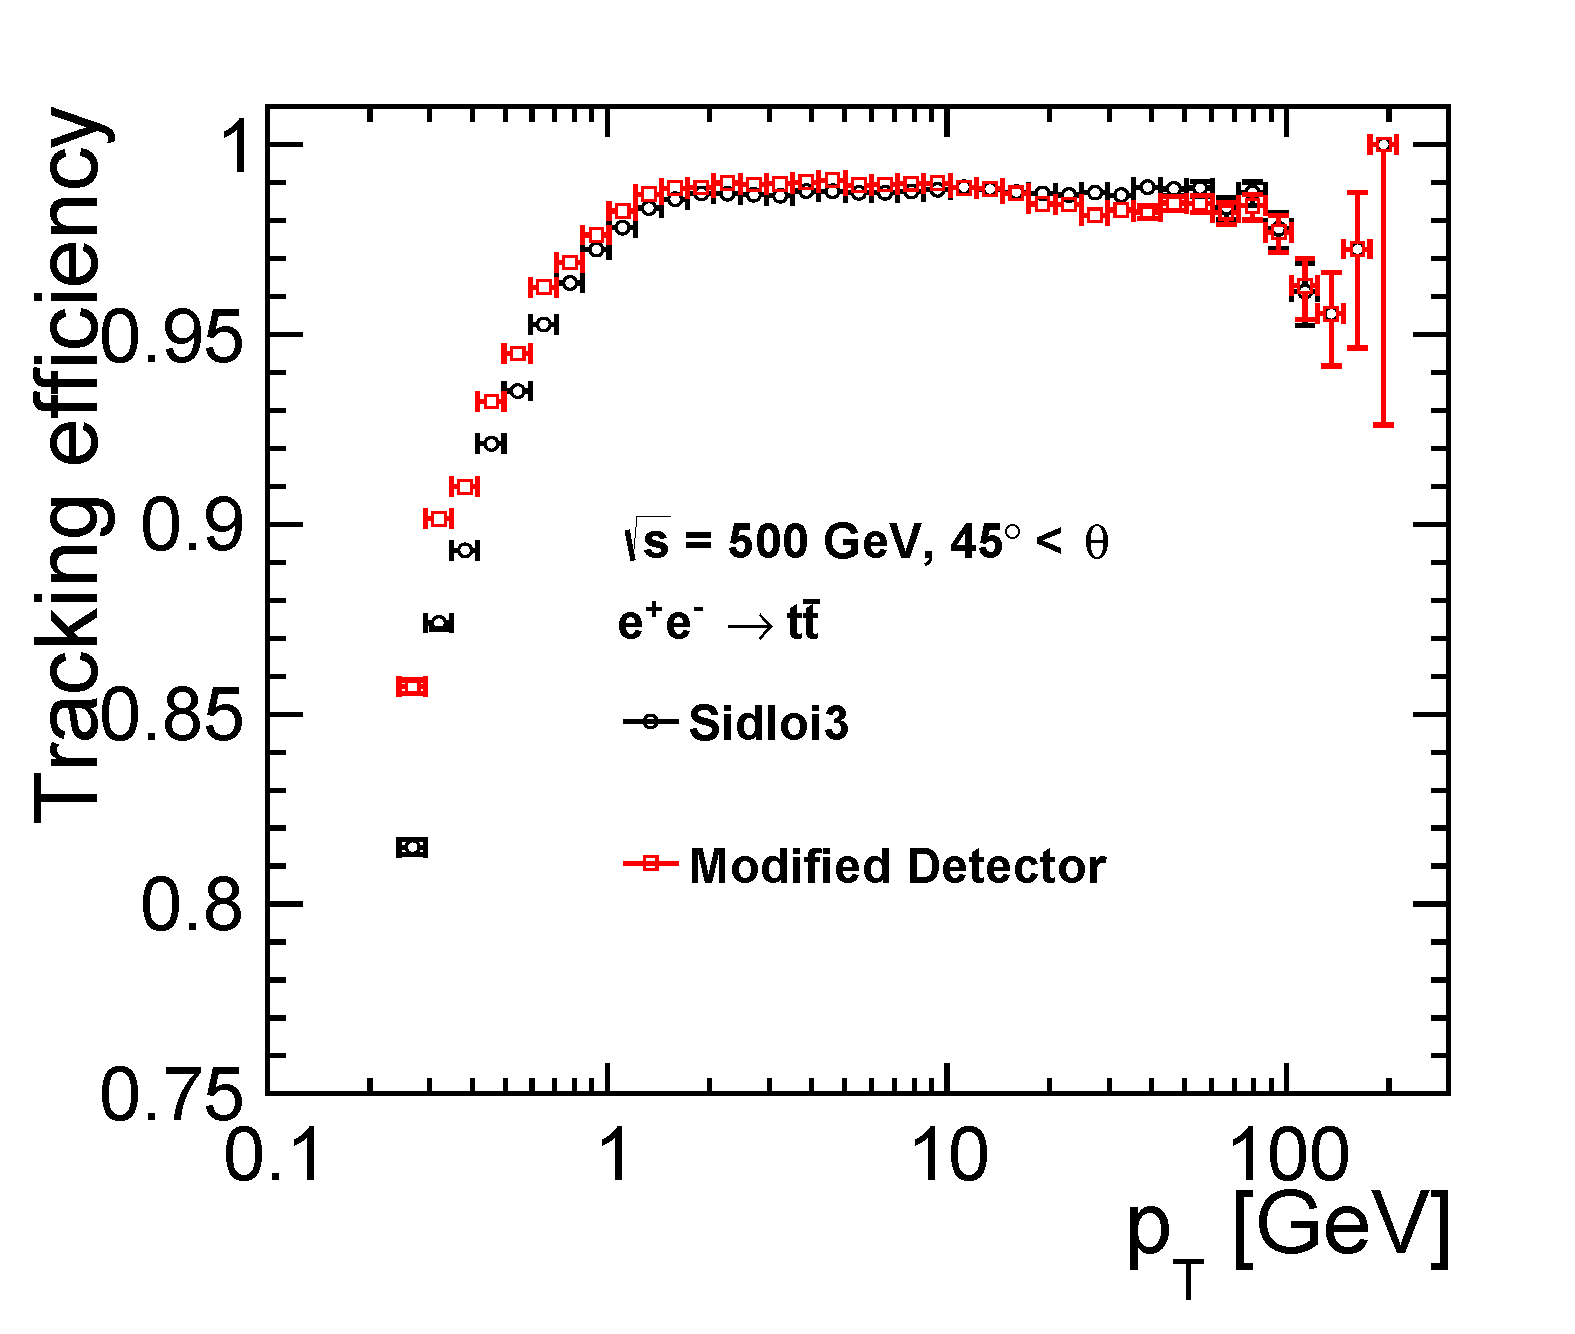
\includegraphics[width=2.0in]{eettbarEfficiencyPtHighTheta_sidloi3_det_vtxbar_3doublet.png}
\subcaption{$45^{\circ}< \theta$}\label{fig:eettbareffpthightheta}
\end{minipage}
\caption{Tracking efficiency for $\ee \rightarrow \ttbar$ at $ \sqrt{s} = $ 500 GeV as a function of transverse momentum
for particles at (a) $10^{\circ}< \theta < 20^{\circ}$, (b) $20^{\circ}< \theta < 45^{\circ}$V, and (c) $45^{\circ}< \theta$.}
\label{fig:eettbareffpt}
\end{figure}

Figure~\ref{fig:eettbareffhitdist} illustrates the tracking efficiency for $\ee \rightarrow \ttbar$ events as a function of the number hits
generated by the Monte Carlo charged particle (figure~\ref{fig:eettbareffhit})
and as a function of the distance to the closest hit of a different particle (figure~\ref{fig:eettbareffdistance}).
Figure~\ref{fig:eettbareffhit} illustrates that the modified detector has worse tracking efficiency
for particles with $<$ 12 hits.
For particles with 12 hits, both detectors perform equally well, with efficiencies near 100\%.
The efficiency for both detectors drops for tracks with more than 12 hits, 
with the modified detector performing somewhat better for particles that produce 14 and 15 hits.
The tracking efficiency with respect to the distance to the closest hit
from another charged particle (figure~\ref{fig:eettbareffdistance}) is nearly equivalent for both detectors.
%%%efficiency hits distance
\begin{figure}[h!]
\begin{minipage}{.5\textwidth}
\centering
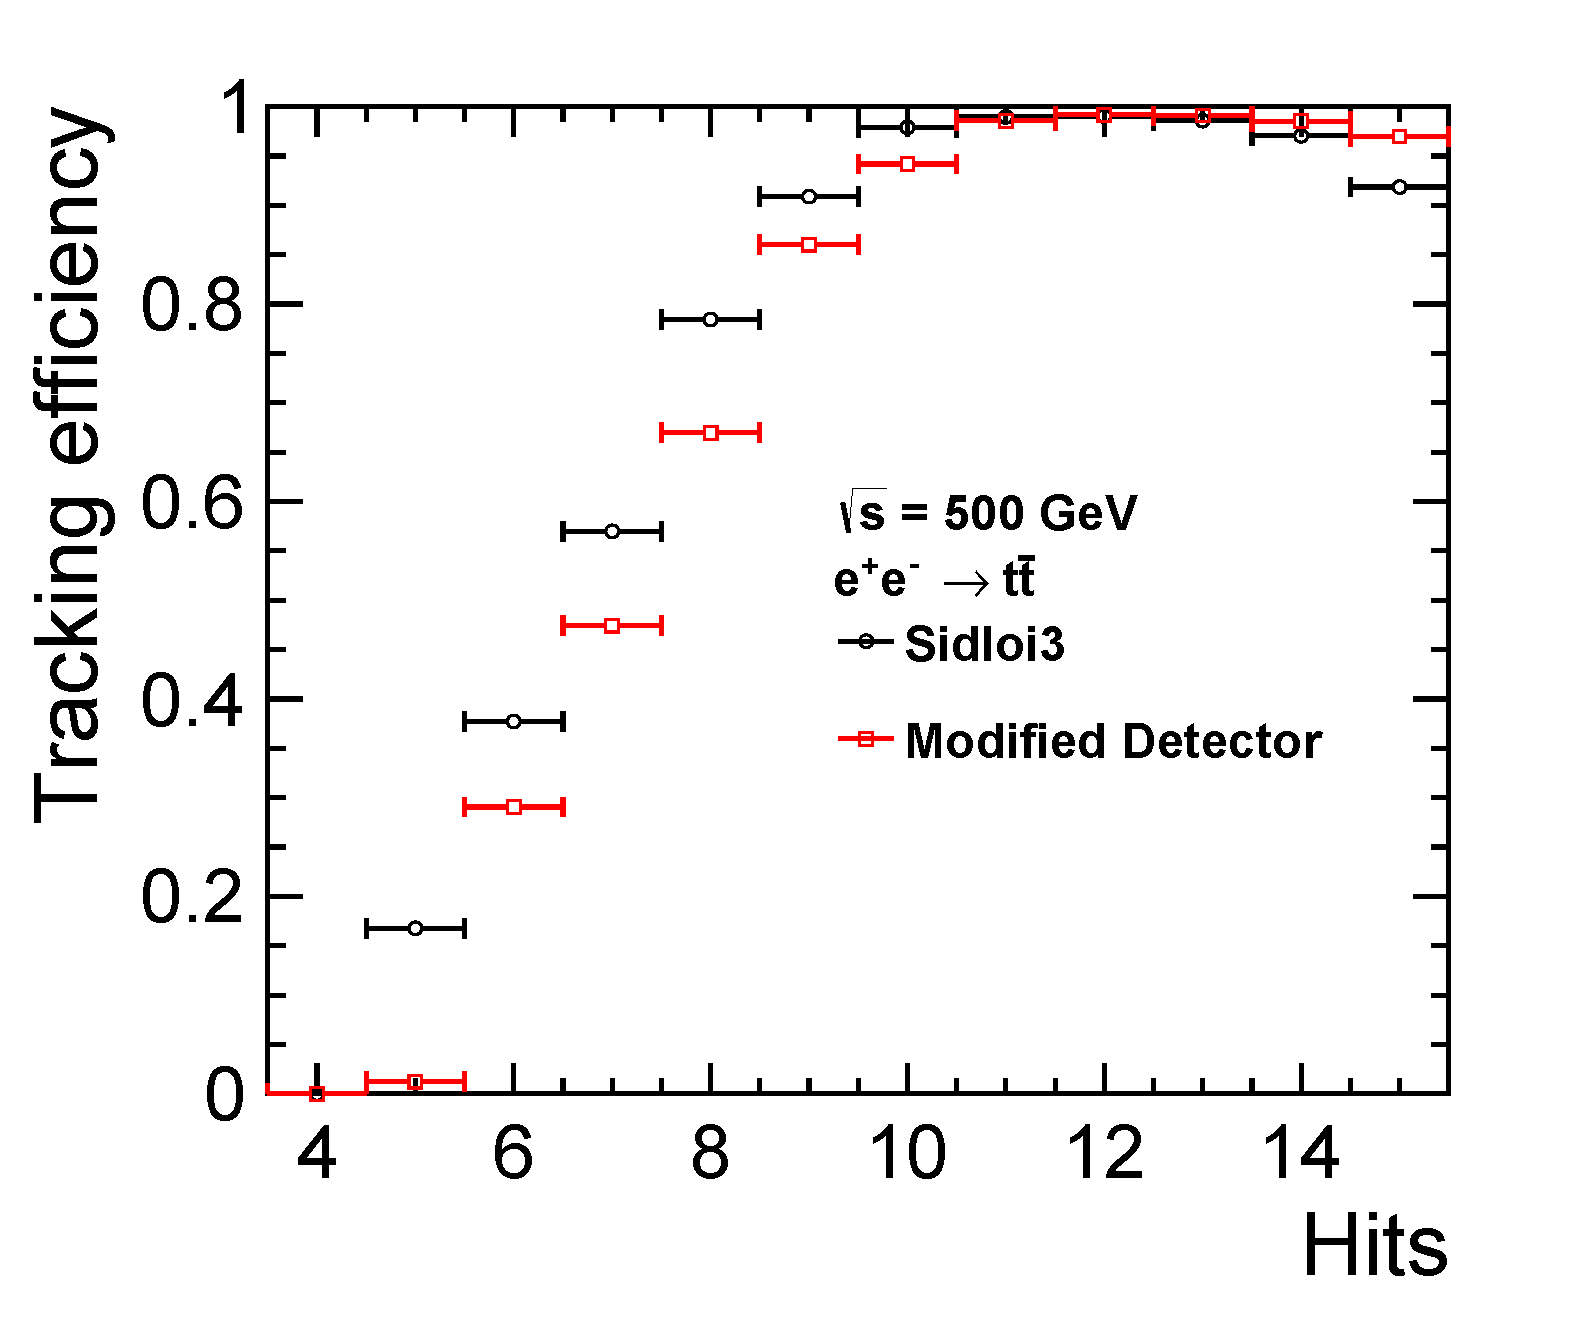
\includegraphics[width=3.0in]{eettbarEfficiencyHits_sidloi3_det_vtxbar_3doublet.png}
\subcaption{Efficiency vs.~Hits}\label{fig:eettbareffhit}
\end{minipage}
\begin{minipage}{.5\textwidth}
\centering
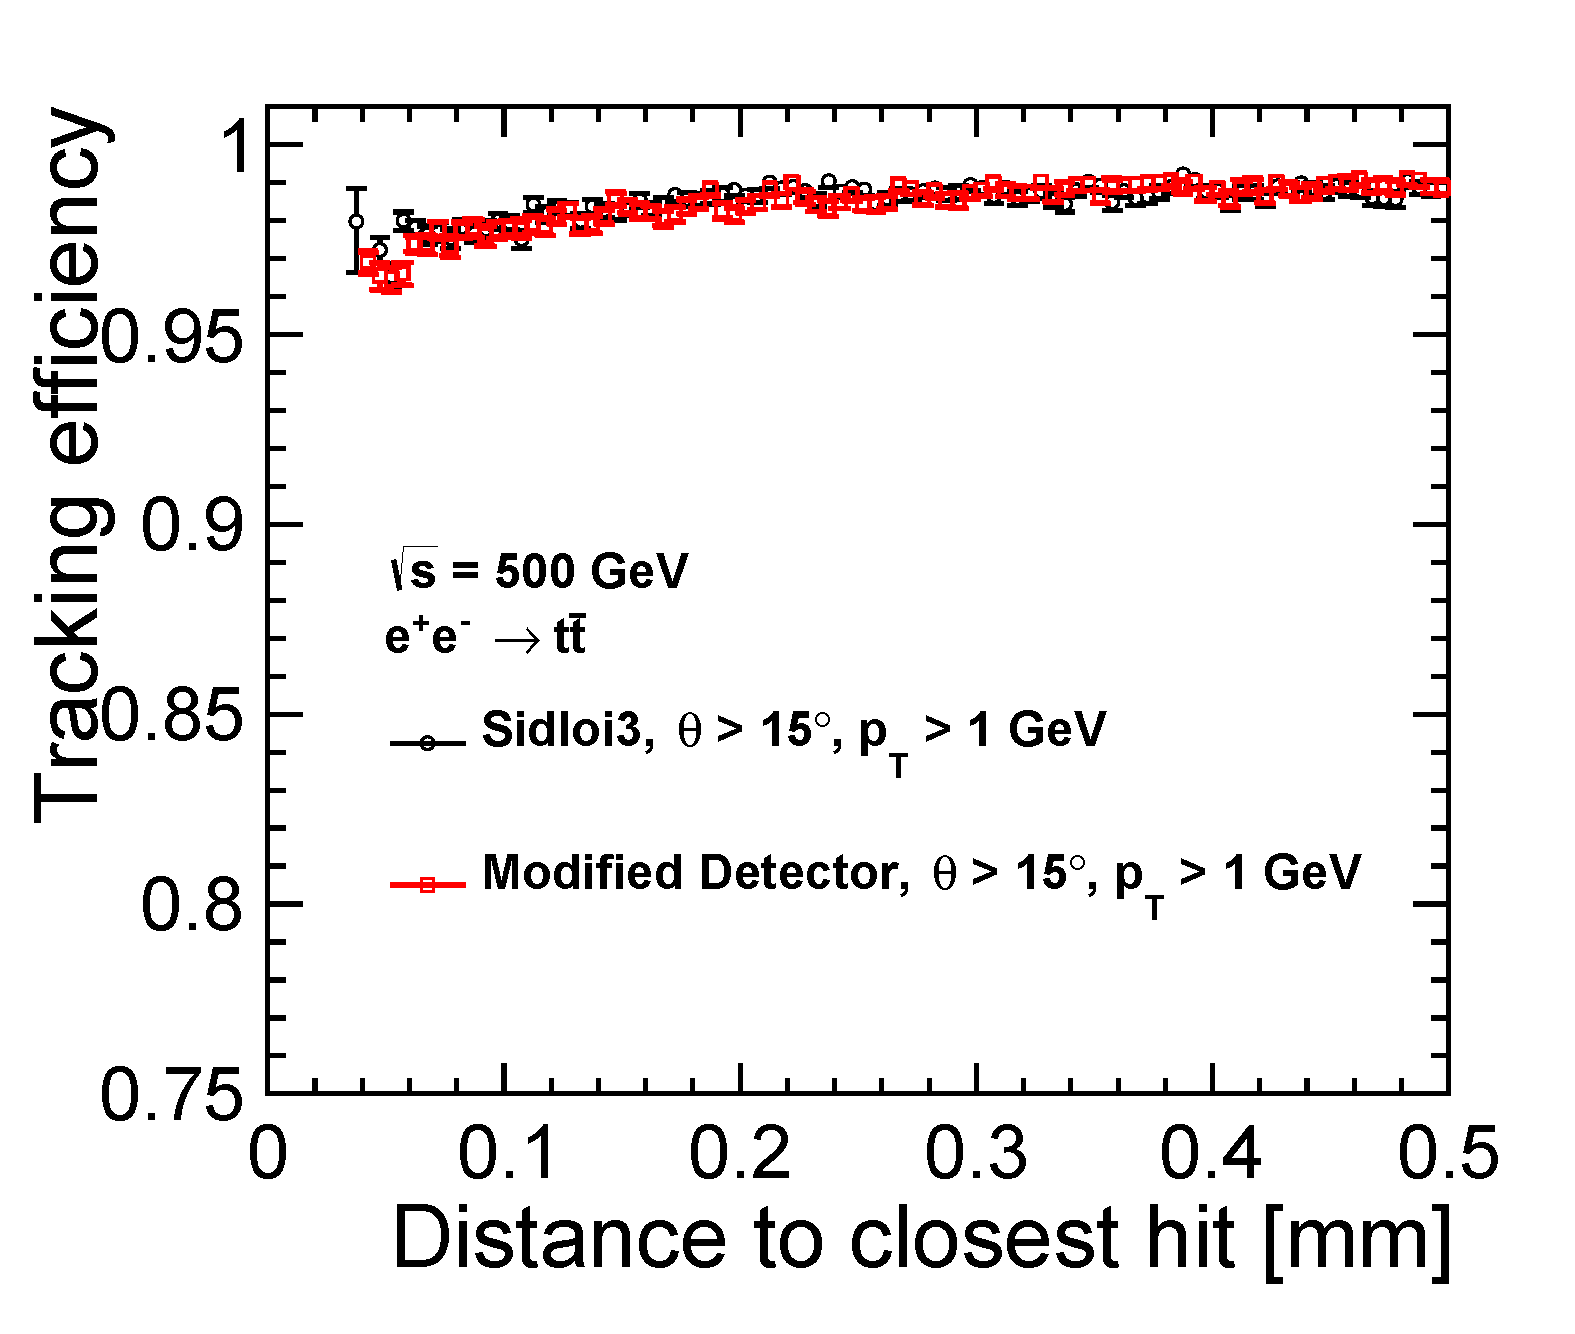
\includegraphics[width=3.0in]{eettbarEfficiencyDistance_sidloi3_det_vtxbar_3doublet.png}
\subcaption{Efficiency vs.~Distance To Closest Hit}\label{fig:eettbareffdistance}
\end{minipage}
\caption{Tracking efficiency for $\ee \rightarrow \ttbar$ at $ \sqrt{s} = $ 500 GeV as a function of (a) the total number
hits generated by the Monte Carlo charged particle and (b) the distance to the closest hit generated by a different particle.}
\label{fig:eettbareffhitdist}
\end{figure}

\subsubsection{$\ee \rightarrow \ttbar \bbbar$ (hadronic decays only), $ \sqrt{s} = $ 1 TeV}
The tracking efficiencies for $\ee \rightarrow \ttbar \bbbar$ events at $ \sqrt{s} = $ 1 TeV
 display most of the same trends as did
the tracking efficiencies for the $ \sqrt{s} = $ 500 GeV $\ee \rightarrow \ttbar$ events, albeit with some minor differences.
To begin, the modified detector once again had greater efficiency for
low transverse momentum particles (0.5 GeV $< p_{T} < $ 2 GeV) for large polar angles ($\theta > 30^{\circ}$),
as shown in figure~\ref{fig:ttbbeffthetalowpt}.
In addition, the modified detector again had lower efficiency than Sidloi3 for 
higher transverse momentum (30 GeV $< p_{T} $) particles at $\theta > 60^{\circ}$ (figure~\ref{fig:ttbbeffthetahighpt}).
Both results are similar to what is seen with the $\ee \rightarrow \ttbar$ events in figure~\ref{fig:eettbareffthetalowpt}
and figure~\ref{fig:eettbareffthetahighpt}, respectively.
However, in the case of $\ee \rightarrow \ttbar \bbbar$ events, both detectors had
equal tracking efficiencies for particles with transverse momentum 2 GeV $< p_{T} < $ 30 GeV (figure~\ref{fig:ttbbeffthetamedpt})
at polar angles $\theta > 45^{\circ}$.
This is not the case for $\ee \rightarrow \ttbar$ events (figure~\ref{fig:eettbareffthetamedpt}), in which
the modified detector has greater efficiency than Sidloi3
for particles with transverse momentum 2 GeV $< p_{T} < $ 30 GeV at polar angles $\theta > 45^{\circ}$.
Still, note that there is a narrow polar angle region ($30^{\circ} < \theta < 45^{\circ}$) in 
figure~\ref{fig:ttbbeffthetamedpt} in which the modified detector
did perform better than Sidloi3, which agrees with the performance as shown for the $\ee \rightarrow \ttbar$ events 
in figure~\ref{fig:eettbareffthetamedpt} for that polar angle region.
%%% efficiency theta
\begin{figure}[h!]
\begin{minipage}{.33\textwidth}
\centering
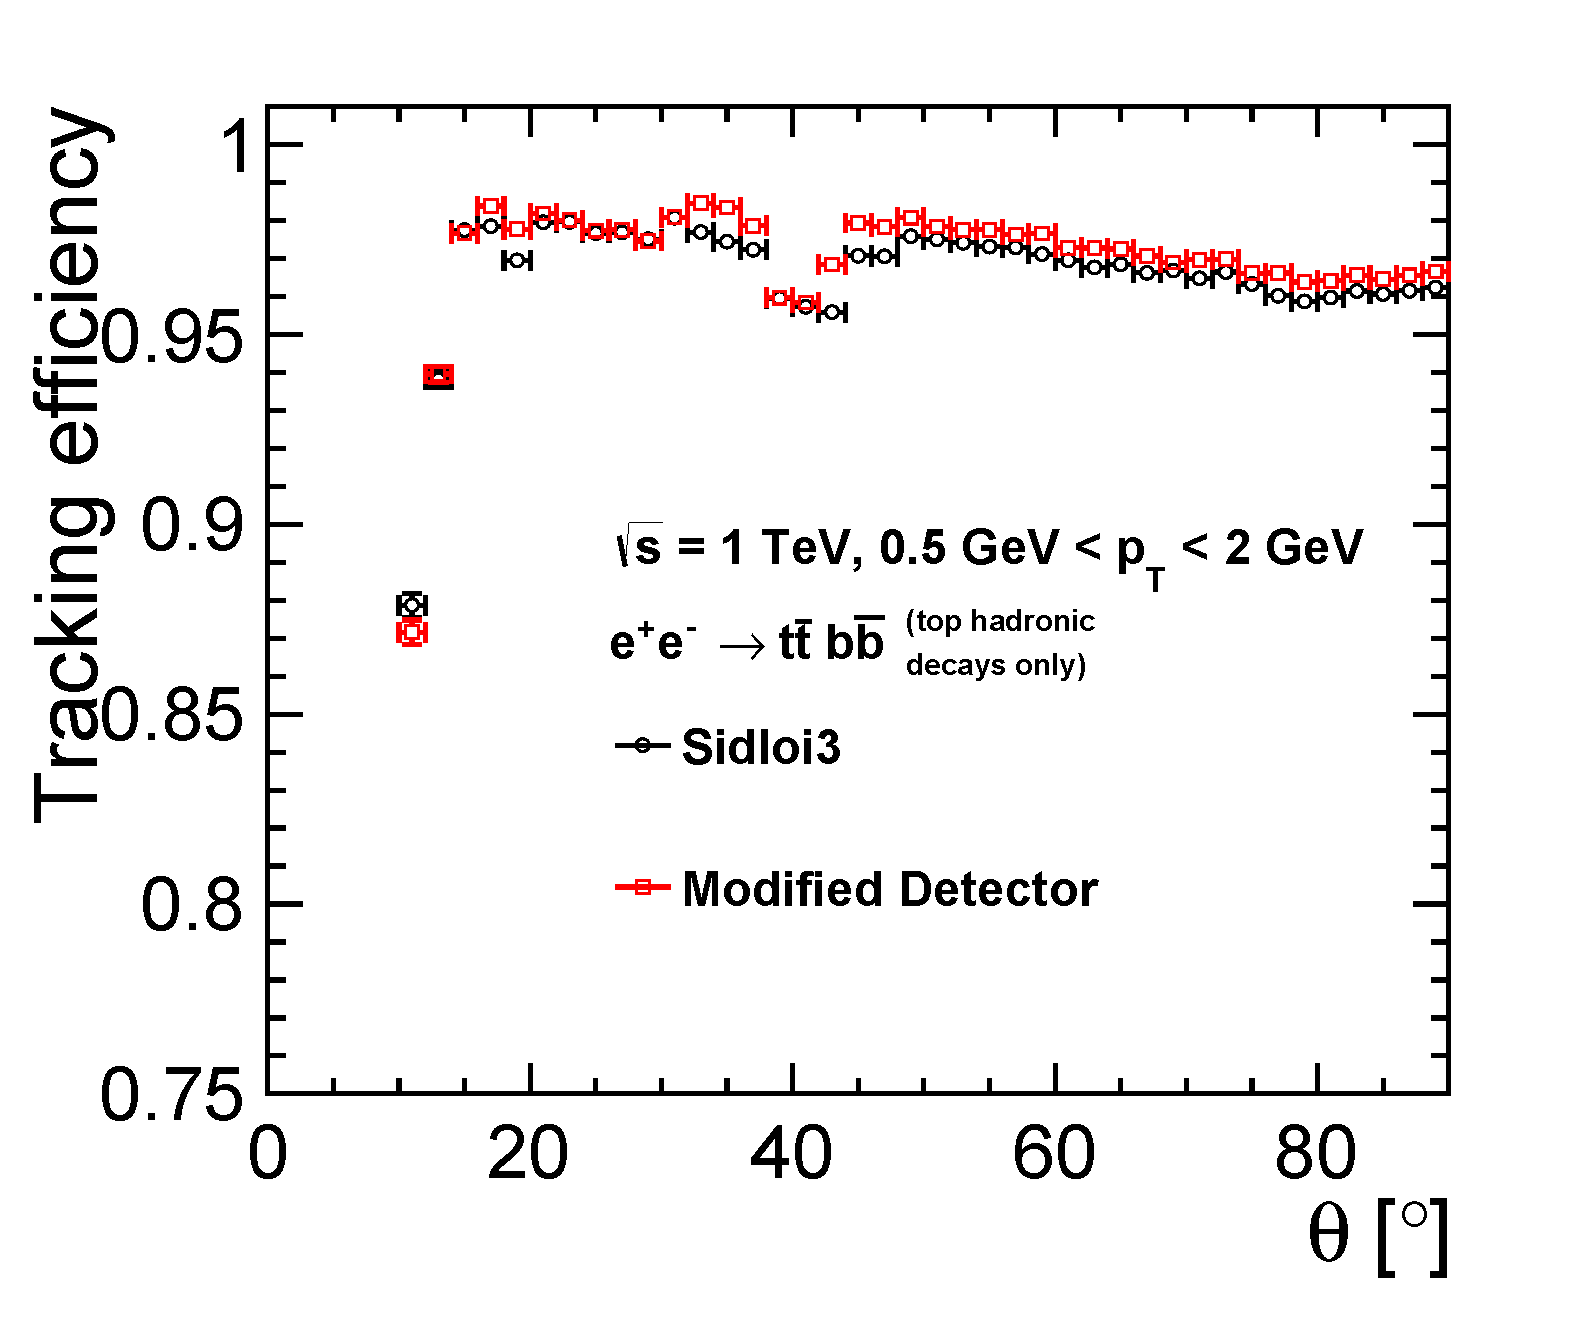
\includegraphics[width=2.0in]{ttbb6qallEfficiencyThetaLowPt_sidloi3_det_vtxbar_3doublet.png}
\subcaption{0.5 GeV $< p_{T} < $ 2 GeV}\label{fig:ttbbeffthetalowpt}
\end{minipage}%
\begin{minipage}{.33\textwidth}
\centering
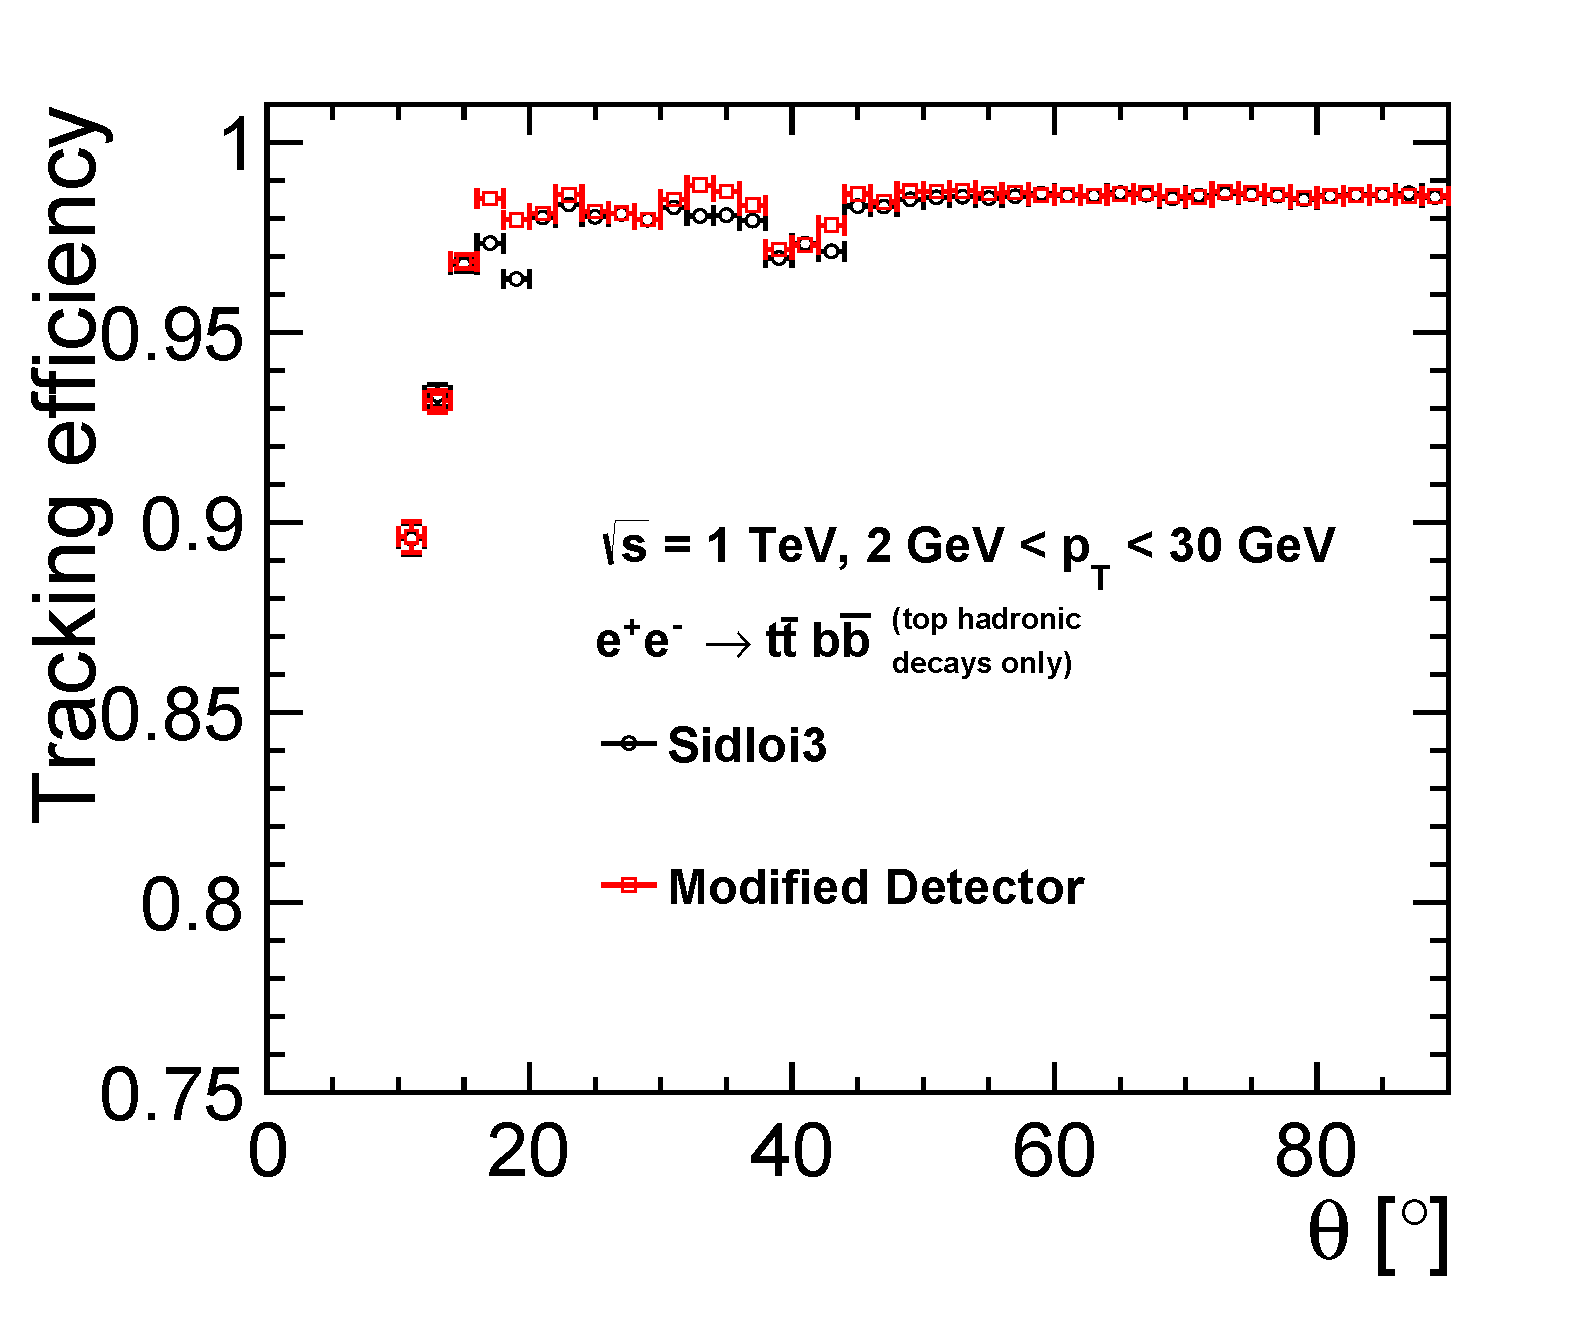
\includegraphics[width=2.0in]{ttbb6qallEfficiencyThetaMedPt_sidloi3_det_vtxbar_3doublet.png}
\subcaption{2 GeV $< p_{T} < $ 30 GeV}\label{fig:ttbbeffthetamedpt}
\end{minipage}
\begin{minipage}{.33\textwidth}
\centering
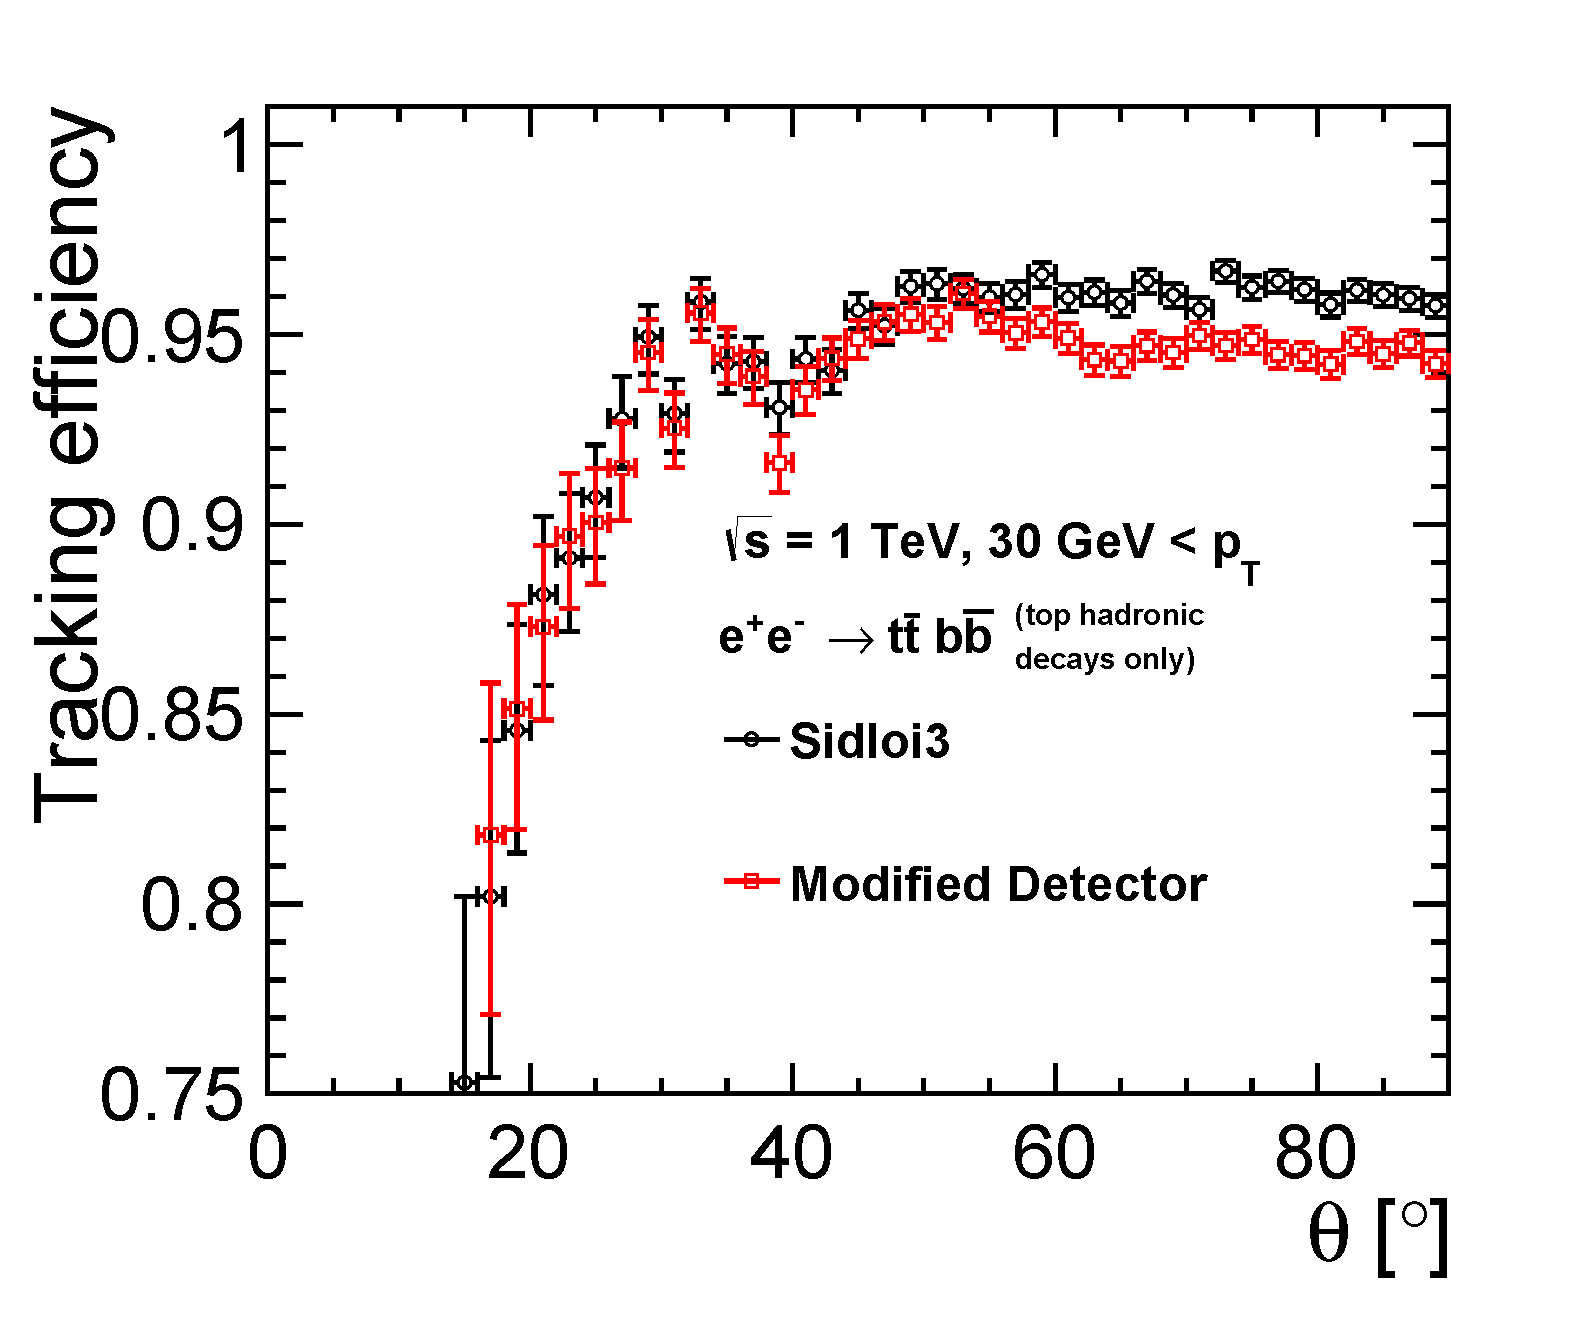
\includegraphics[width=2.0in]{ttbb6qallEfficiencyTheta30GeV_sidloi3_det_vtxbar_3doublet.png}
\subcaption{30 GeV $< p_{T} $}\label{fig:ttbbeffthetahighpt}
\end{minipage}
\caption{Tracking efficiency for $\ee \rightarrow \ttbar \bbbar$ (hadronic decays only) at $ \sqrt{s} = $ 1 TeV as a function of polar angle
for (a) 0.5 GeV $< p_{T} < $ 2 GeV, (b) 2 GeV $< p_{T} < $ 30 GeV, and (c) 30 GeV $< p_{T} $ particles.}
\label{fig:ttbbefftheta}
\end{figure}

Figure~\ref{fig:ttbbeffpt}, in which efficiency is plotted versus transverse momentum for $\ee \rightarrow \ttbar \bbbar$,
supports the trends seen in figure~\ref{fig:ttbbefftheta}.
Figure~\ref{fig:ttbbeffpthightheta} illustrates that
the modified detector has worse efficiency for 
higher transverse momentum particles ($p_{T} > $20 GeV)
at high polar angles ($\theta > 45^{\circ}$).
Figure~\ref{fig:ttbbeffpthightheta} and figure~\ref{fig:ttbbeffptmedtheta} also illustrate 
that the modified detector has better efficiency for
 lower transverse momentum (0.2 GeV $< p_{T} <$ 1 GeV) particles at a wide polar angle ($\theta > 20^{\circ}$).
In addition, the modified detector demonstrates slightly better efficiency 
for 1 GeV $< p_{T} <$ 10 GeV particles at $20^{\circ} < \theta < 45^{\circ}$,
as shown in figure~\ref{fig:ttbbeffptmedtheta}.
Unlike for the $\ee \rightarrow \ttbar$ events as shown in figure~\ref{fig:eettbareffptlowtheta}, the modified detector's improved efficiency
for low transverse momentum (0.2 GeV $< p_{T} <$ 2 GeV)  particles does not extend to low polar angles ($10^{\circ} < \theta < 20^{\circ}$)
for $\ee \rightarrow \ttbar \bbbar$ events
as is evident in  figure~\ref{fig:ttbbeffptlowtheta}.
Still, figure~\ref{fig:ttbbeffptlowtheta} indicates that the modified detector does have better
efficiency for particles with slightly higher transverse momentum (2 GeV $< p_{T}<$20 GeV)
at low polar angles ($10^{\circ} < \theta < 20^{\circ}$), which agrees with figure~\ref{fig:ttbbefftheta}.
%%% efficiency pt
\begin{figure}[h!]
\begin{minipage}{.33\textwidth}
\centering
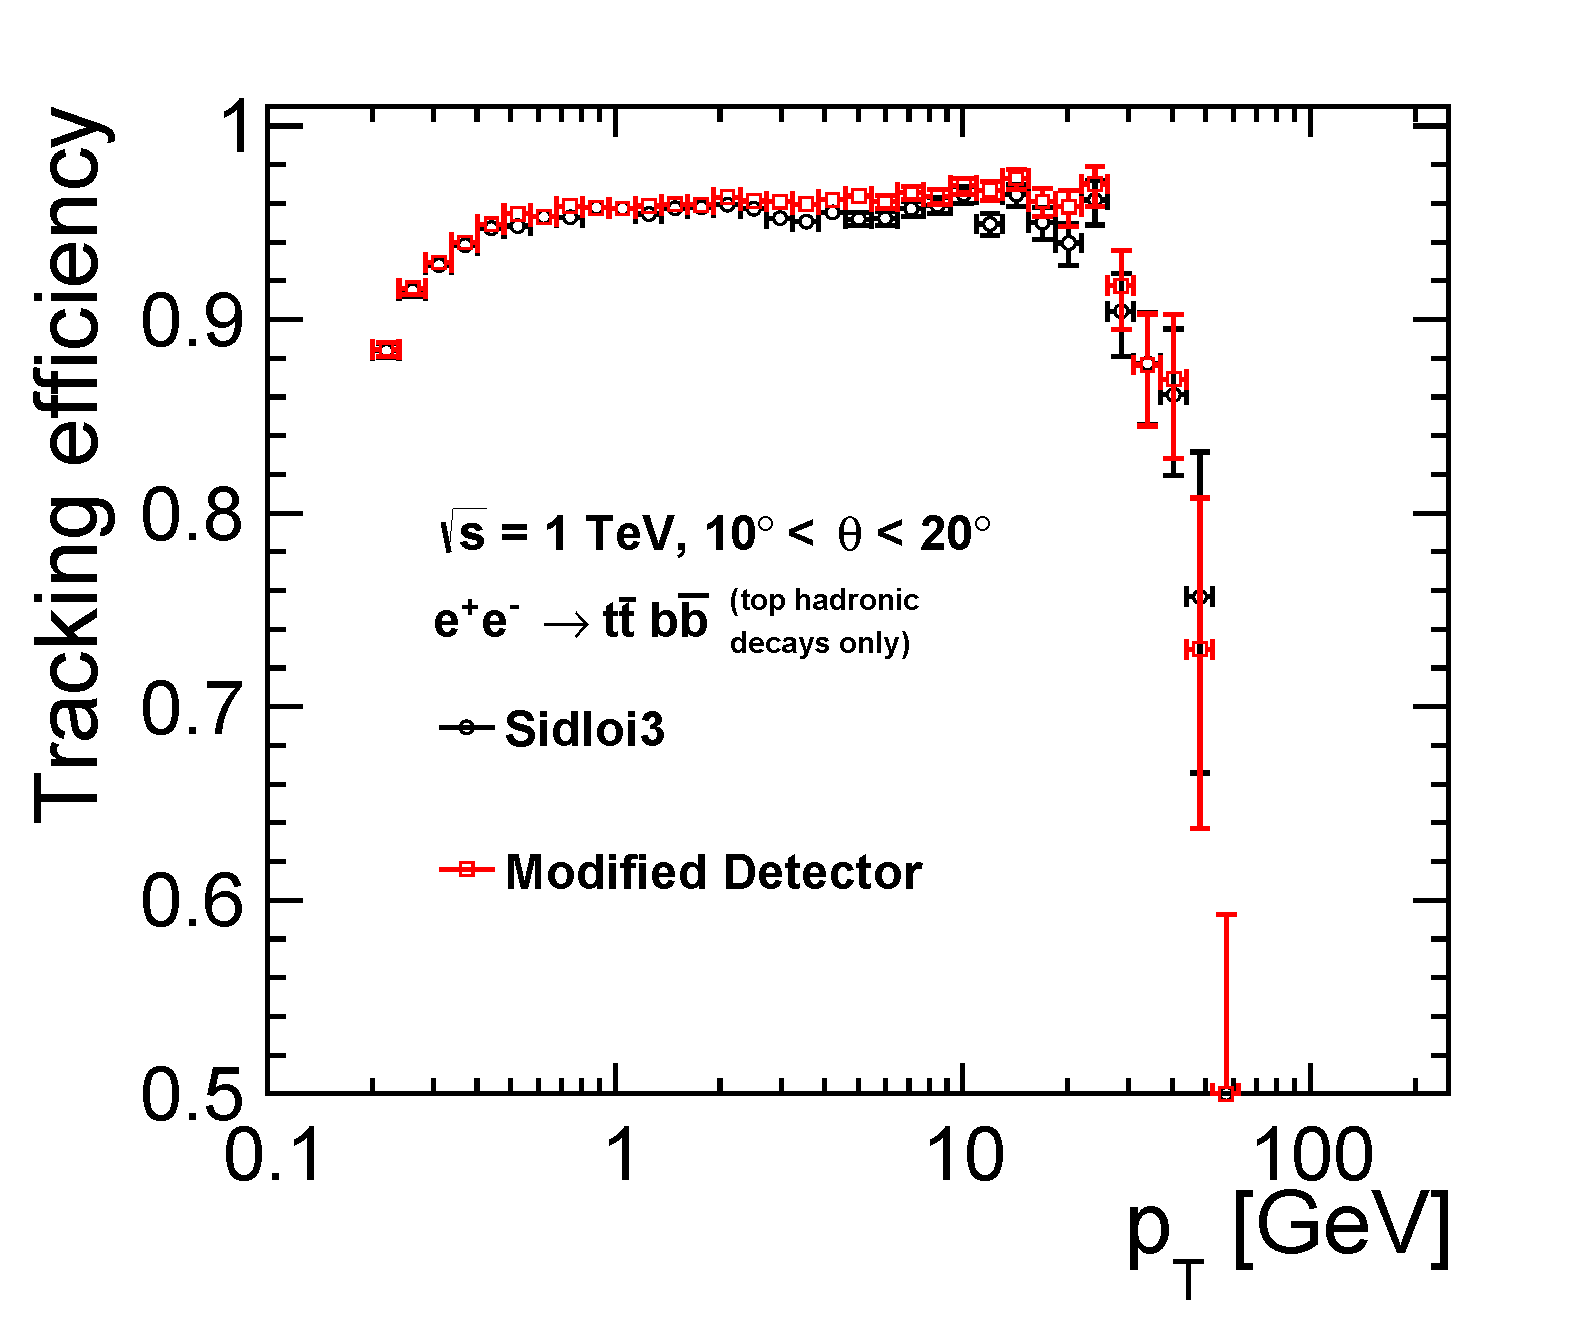
\includegraphics[width=2.0in]{ttbb6qallEfficiencyPtLowTheta_sidloi3_det_vtxbar_3doublet.png}
\subcaption{$10^{\circ}< \theta <  20^{\circ}$}\label{fig:ttbbeffptlowtheta}
\end{minipage}%
\begin{minipage}{.33\textwidth}
\centering
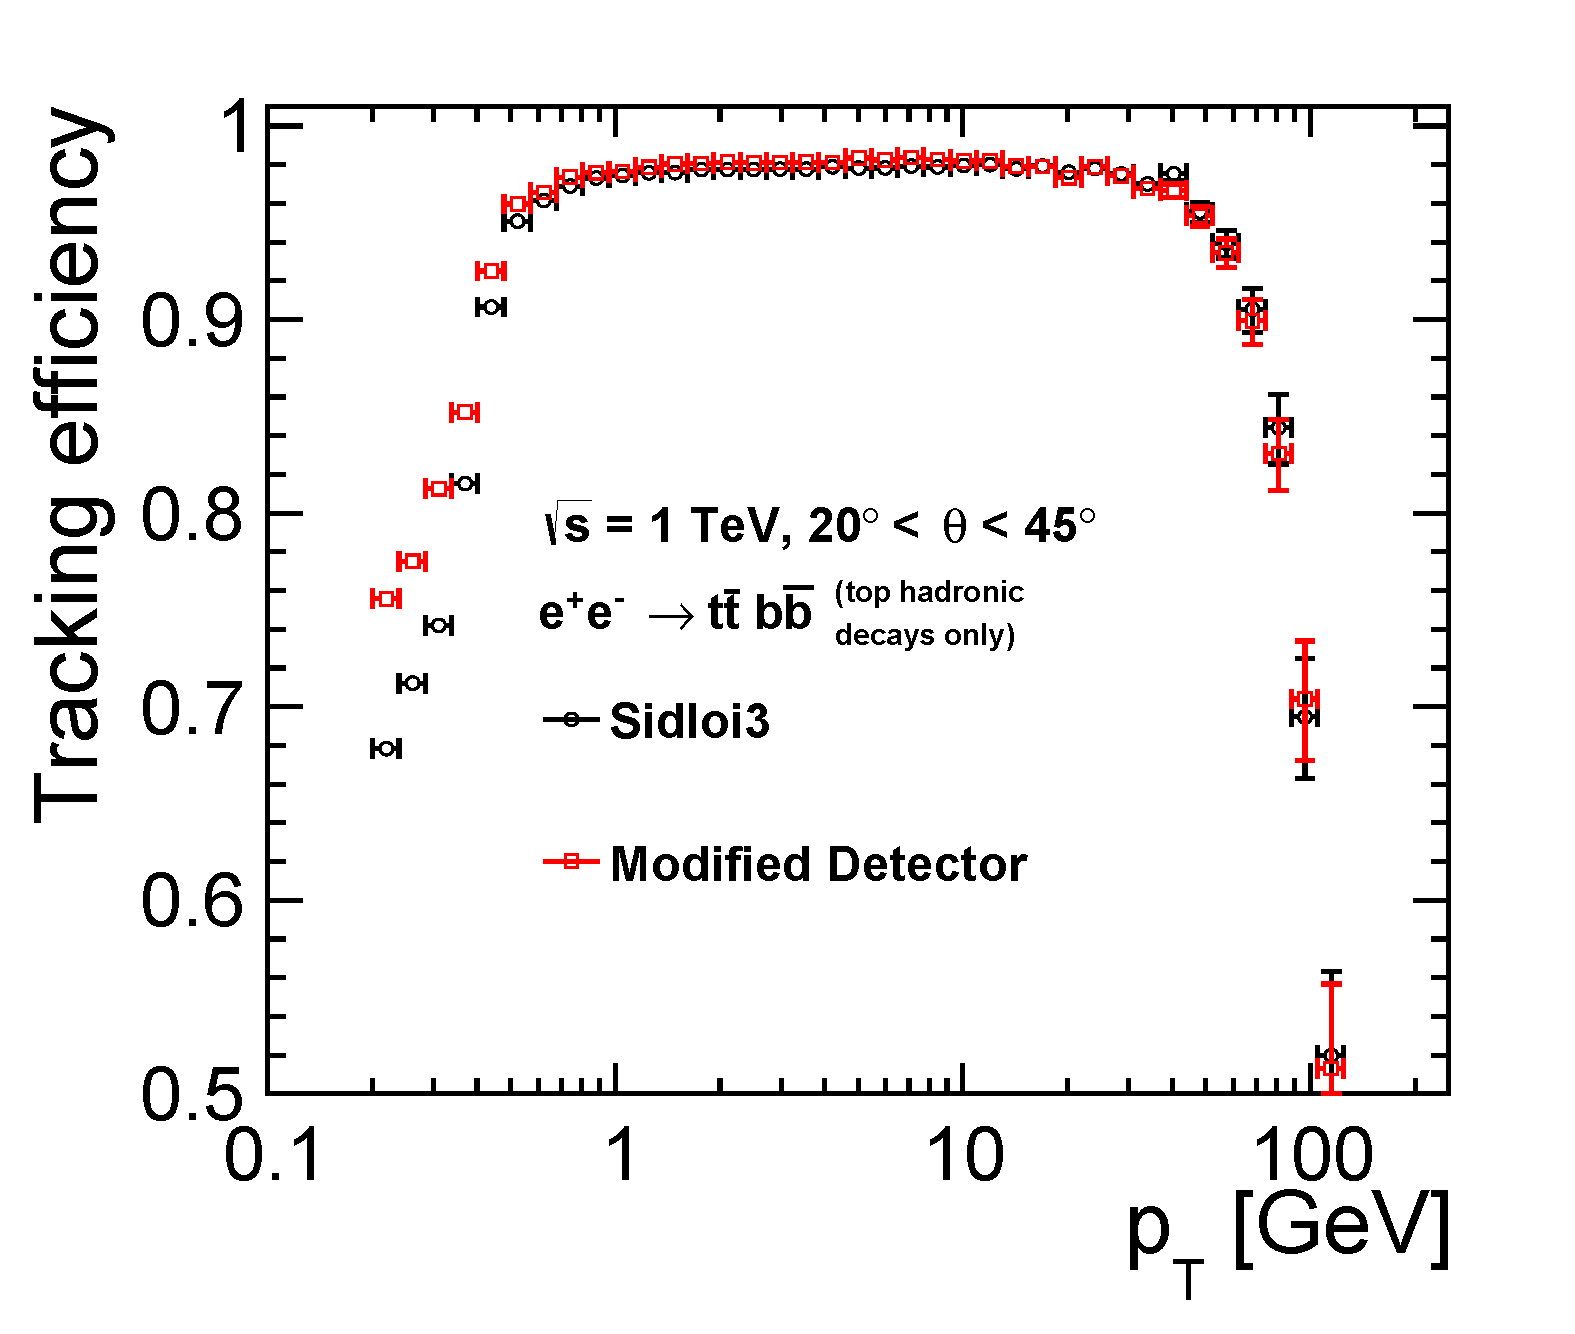
\includegraphics[width=2.0in]{ttbb6qallEfficiencyPtMedTheta_sidloi3_det_vtxbar_3doublet.png}
\subcaption{$20^{\circ}< \theta <  45^{\circ}$}\label{fig:ttbbeffptmedtheta}
\end{minipage}
\begin{minipage}{.33\textwidth}
\centering
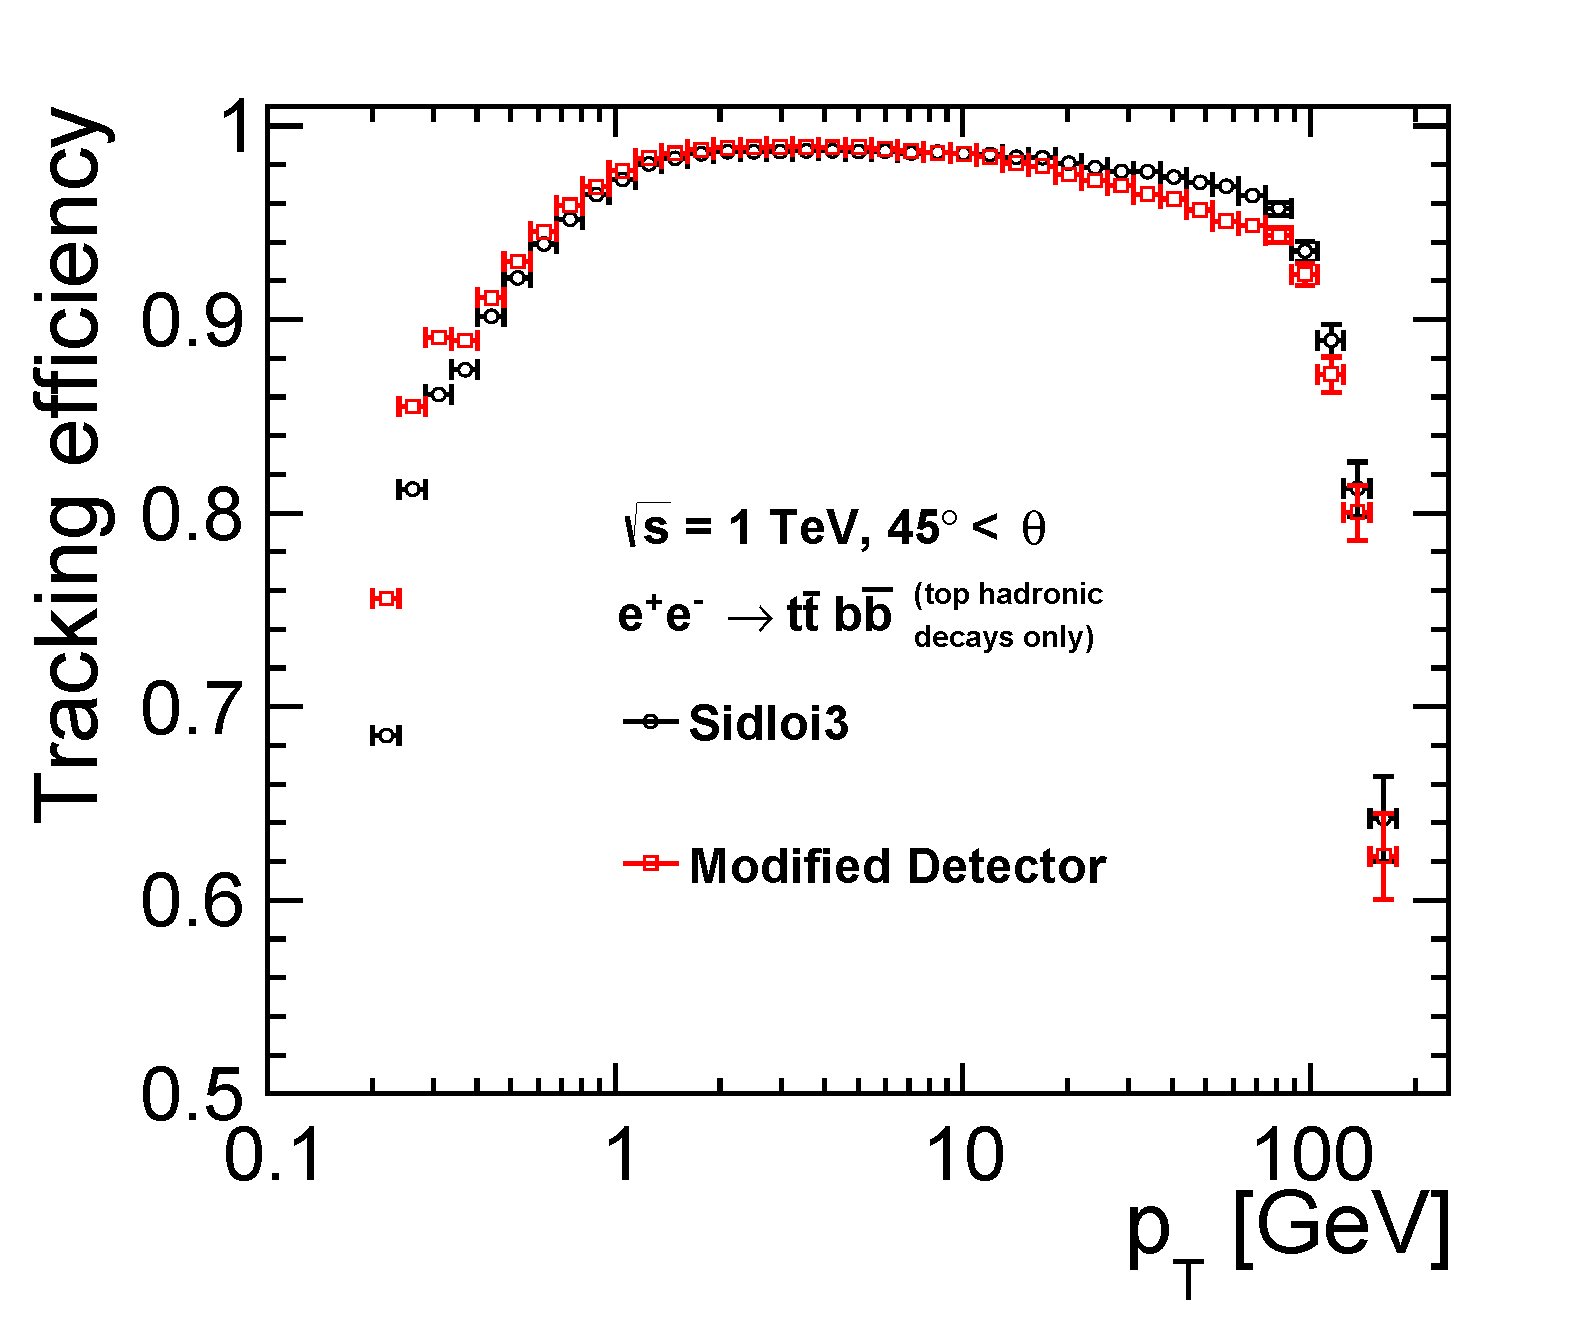
\includegraphics[width=2.0in]{ttbb6qallEfficiencyPtHighTheta_sidloi3_det_vtxbar_3doublet.png}
\subcaption{$45^{\circ}< \theta$}\label{fig:ttbbeffpthightheta}
\end{minipage}
\caption{Tracking efficiency for $\ee \rightarrow \ttbar \bbbar$ (hadronic decays only) at $ \sqrt{s} = $ 1 TeV as a function of transverse momentum
for particles at (a) $10^{\circ}< \theta < 20^{\circ}$, (b) $20^{\circ}< \theta < 45^{\circ}$V, and (c) $45^{\circ}< \theta$.}
\label{fig:ttbbeffpt}
\end{figure}

Efficiency versus total number of hits produced by the Monte Carlo charged particle
is illustrated in figure~\ref{fig:ttbbeffhit} for $\ee \rightarrow \ttbar \bbbar$ events.
Again, the tracking efficiency for the modified detector is worse than that of Sidloi3 for all particles
which generated $<$ 12 hits.
Both detectors have nearly 100\% tracking efficiency for particles generating 12 hits
and slightly less efficiency for particles generating 13 or 14 hits, with the modified detector
performing somewhat better for particles that produced 13 or 14 hits.
This result is nearly identical to those in figure~\ref{fig:eettbareffhit} for $\ee \rightarrow \ttbar$ events.
However, for efficiency versus the distance to the closest hit of a different particle (figure~\ref{fig:ttbbeffdistance}),
the modified detector clearly has worse tracking efficiency than Sidloi3
 from $0.02~mm$ to about $0.22~mm$ for $\ee \rightarrow \ttbar \bbbar$ events.
This stands in contrast to the results in figure~\ref{fig:eettbareffdistance} for the  
$\ee \rightarrow \ttbar$ events, in which both detectors have comparably efficiency with respect to the distance to 
the closest hit from a different particle.
%%%efficiency hits distance
\begin{figure}[h!]
\begin{minipage}{.5\textwidth}
\centering
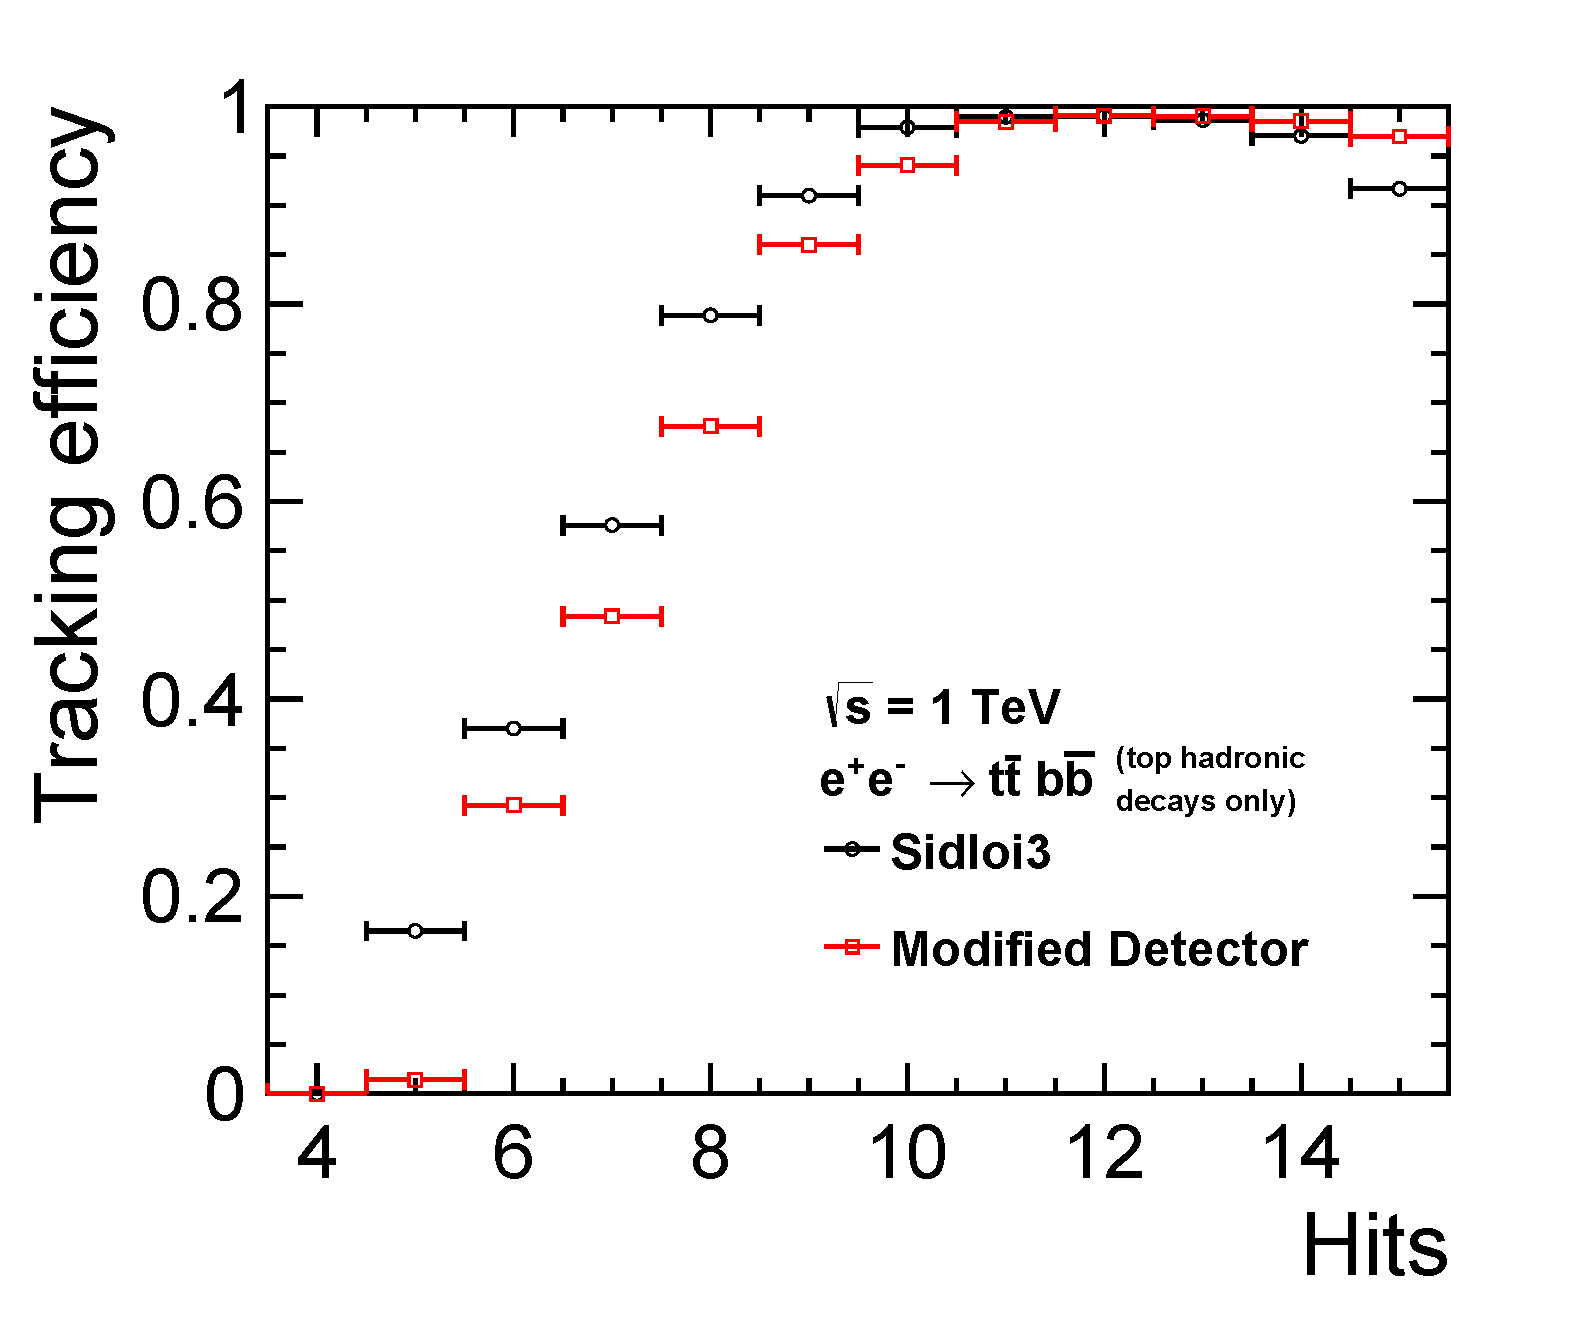
\includegraphics[width=3.0in]{ttbb6qallEfficiencyHits_sidloi3_det_vtxbar_3doublet.png}
\subcaption{Efficiency vs.~Hits}\label{fig:ttbbeffhit}
\end{minipage}
\begin{minipage}{.5\textwidth}
\centering
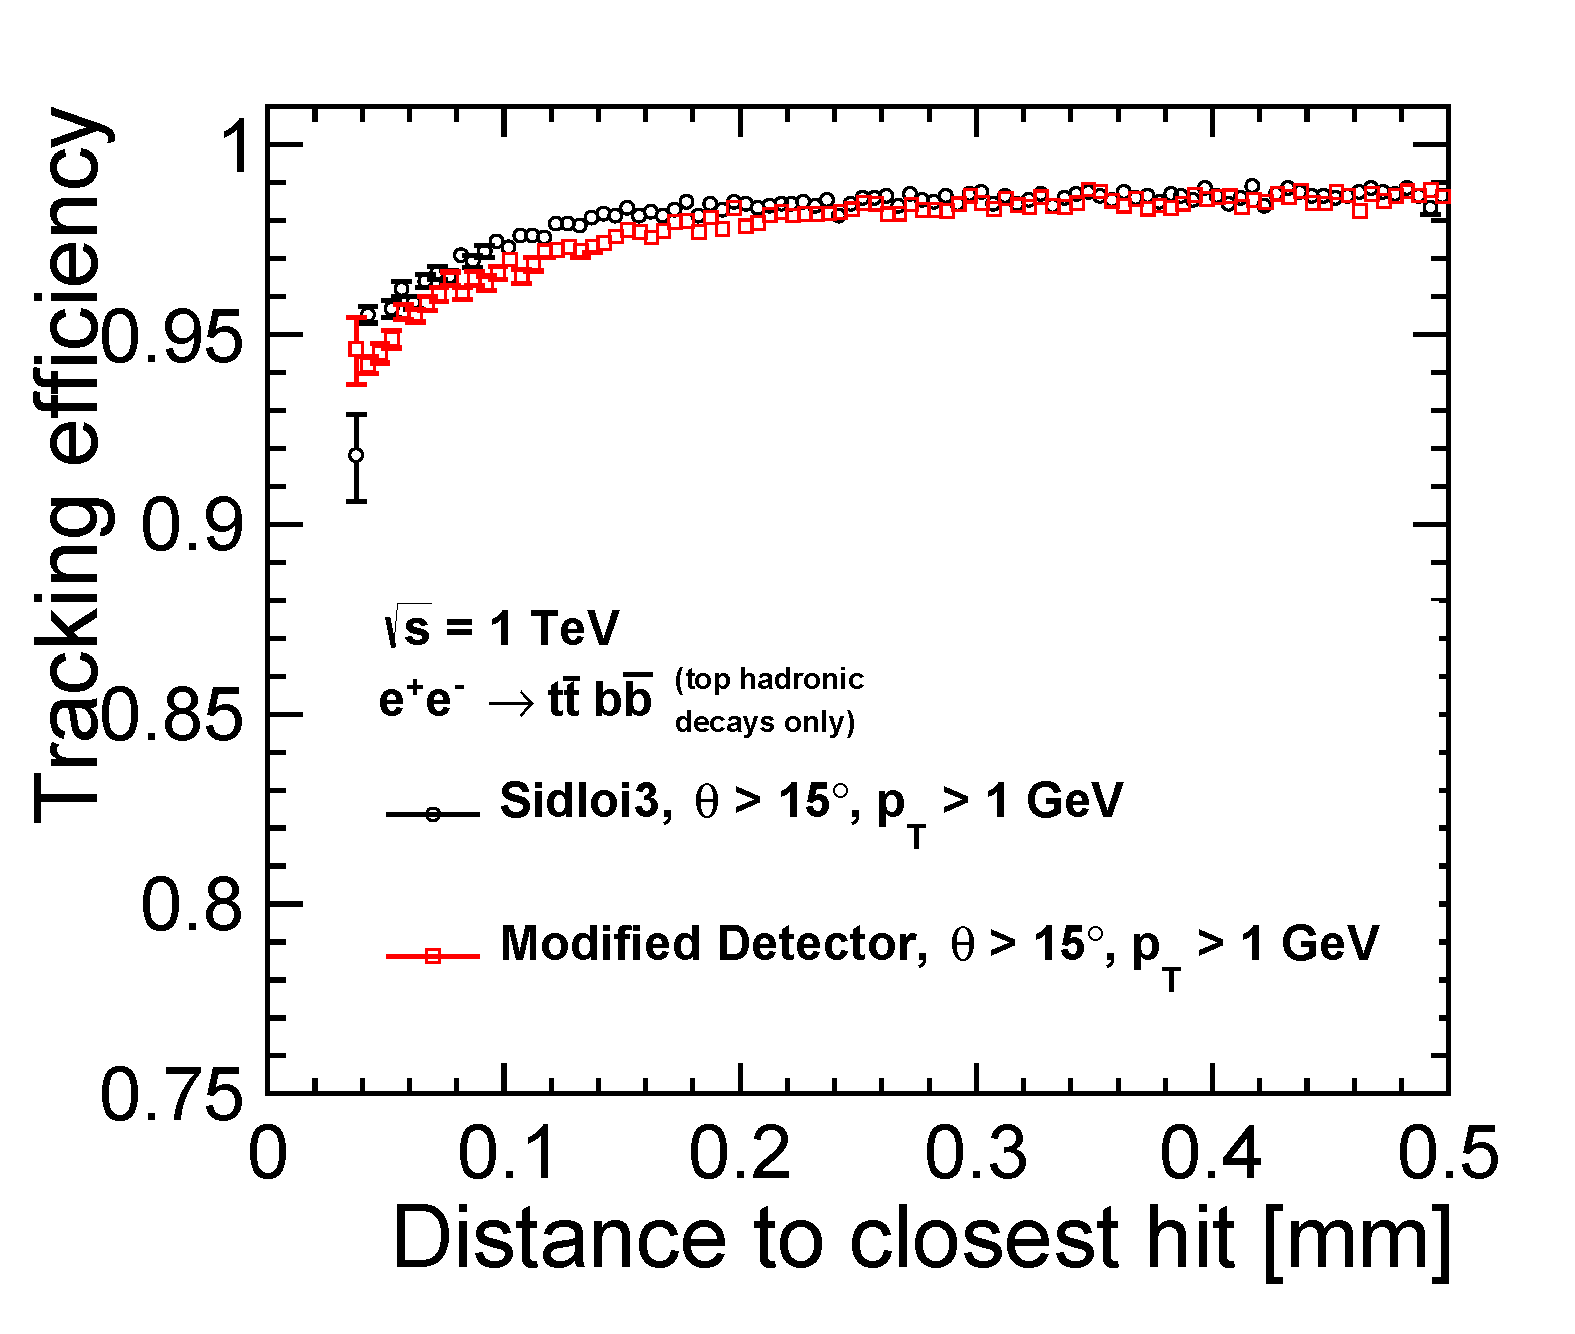
\includegraphics[width=3.0in]{ttbb6qallEfficiencyDistance_sidloi3_det_vtxbar_3doublet.png}
\subcaption{Efficiency vs.~Distance To Closest Hit}\label{fig:ttbbeffdistance}
\end{minipage}
\caption{Tracking efficiency for $\ee \rightarrow \ttbar \bbbar$ (hadronic decays only) at $ \sqrt{s} = $ 1 TeV as a function of (a) the number
hits generated by the Monte Carlo particle associated with the track and (b) the distance from
the track to the closest hit of another track.}
\label{fig:ttbbeffhitdist}
\end{figure}

\subsection{Fake Rates}
The fake rate is defined as the fraction of reconstructed tracks that have greater than one false hit:
\begin{equation}
\mbox{Fake Rate}=\frac{N_{\mbox{\scriptsize{false hits $>$ 1}}}}{N_{\mbox{\scriptsize{reconstructed}}}}.
%\mbox{Efficiency}=\frac{N_{successfully~reconstructed}}{N_{findable}}.
\label{eq:fakerate}
\end{equation}
As figure~\ref{fig:eettbarfakerate} and figure~\ref{fig:ttbbfakerate} indicate, the modified detector
demonstrates higher fake rates for both  $\ee \rightarrow \ttbar$ events at $ \sqrt{s} = $ 500 TeV
and  $\ee \rightarrow \ttbar \bbbar$ events at $ \sqrt{s} = $ 1 TeV
 for polar angles $\theta > 25^{\circ}$ (figures~\ref{fig:eettbarfakeratetheta} and\ref{fig:ttbbfakeratetheta})
and for transverse momentum 0.1 GeV $< p_{T} < $ 200 GeV (figures~\ref{fig:eettbarfakeratept} and \ref{fig:ttbbfakeratept}).
At lower polar angles ($\theta < 25^{\circ}$), the distinction in performance betwee both detectors blurs 
for both types of physics events.
%, with each detector performing comparably(figure~\ref{fig:eettbarfakeratetheta} and figure~\ref{fig:ttbbfakeratetheta}).
%% eettbar fake rate
\begin{figure}
\begin{minipage}{.5\textwidth}
\centering
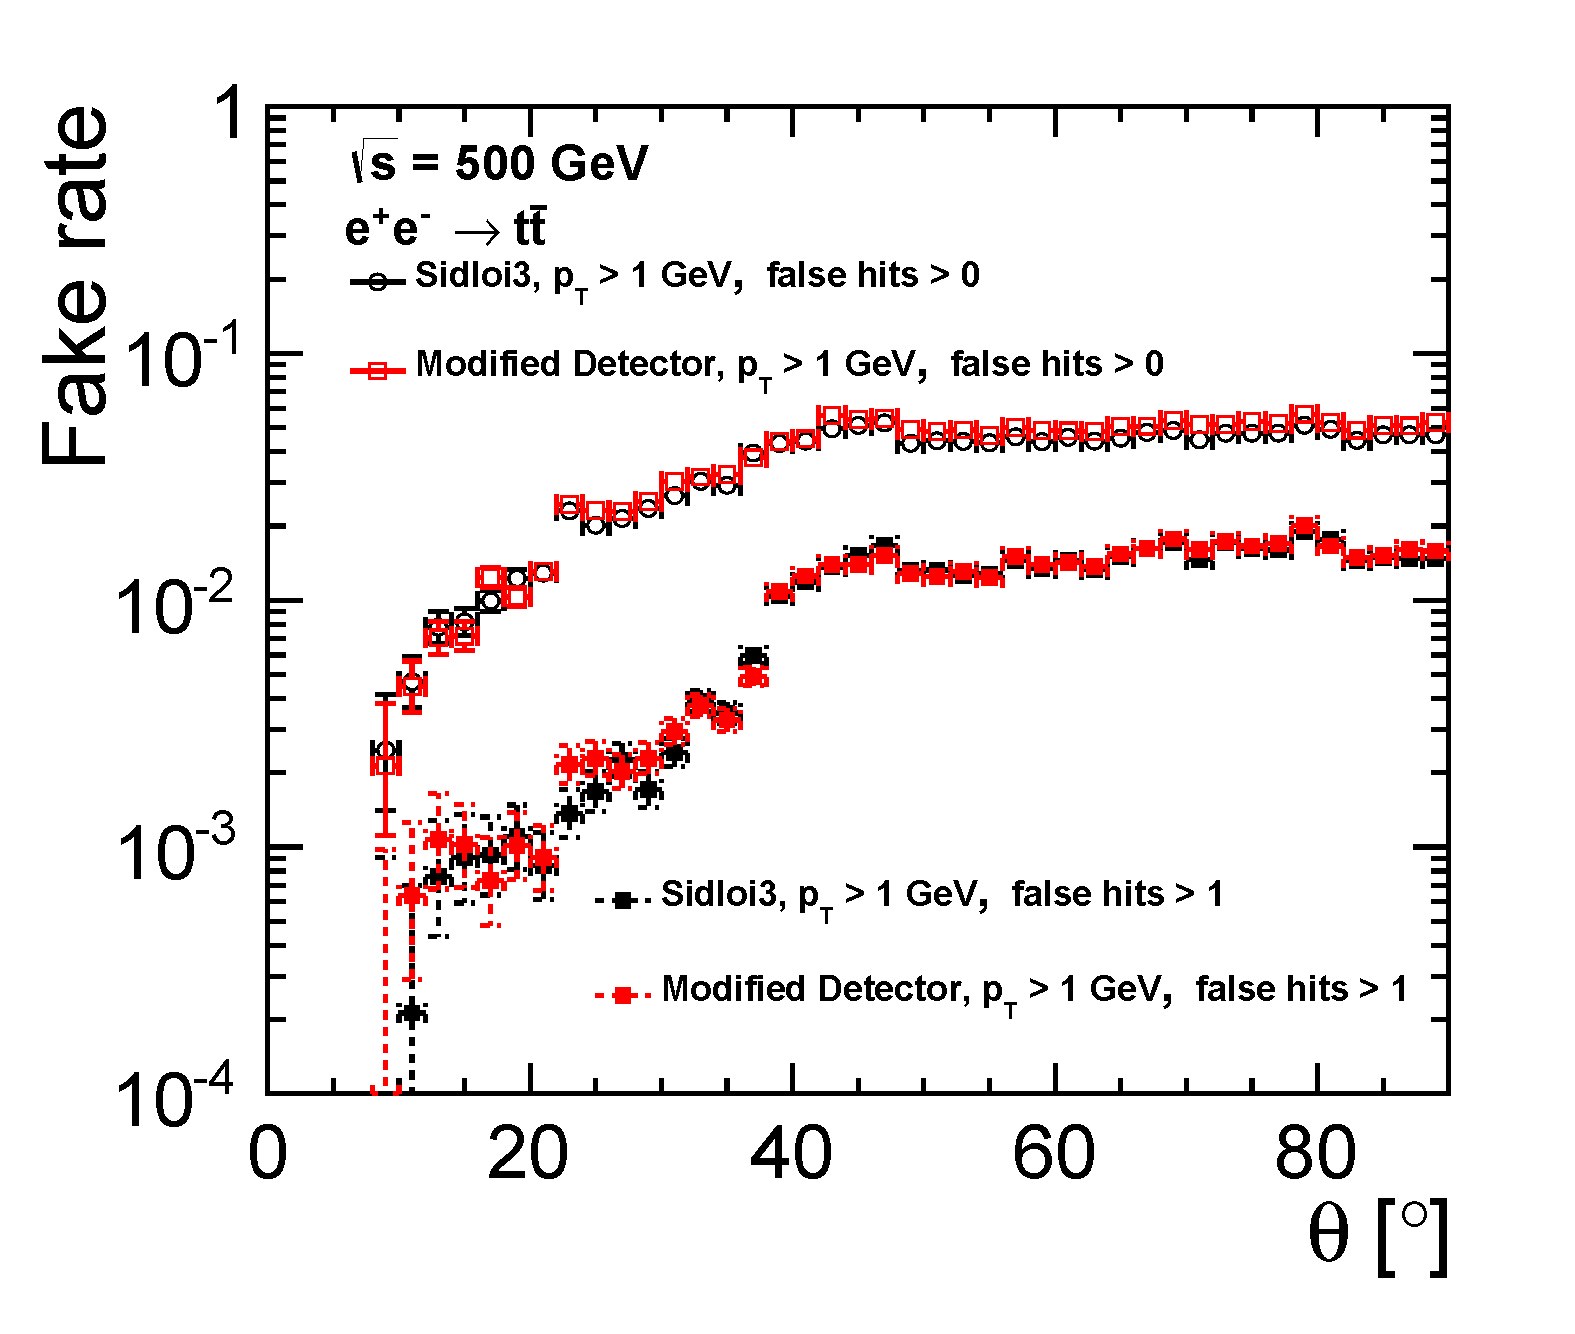
\includegraphics[width=3.0in]{eettbarFakeRateTheta_sidloi3_det_vtxbar_3doublet.png}
\subcaption{Fake Rate vs.~$\theta$}\label{fig:eettbarfakeratetheta}
\end{minipage}
\begin{minipage}{.5\textwidth}
\centering
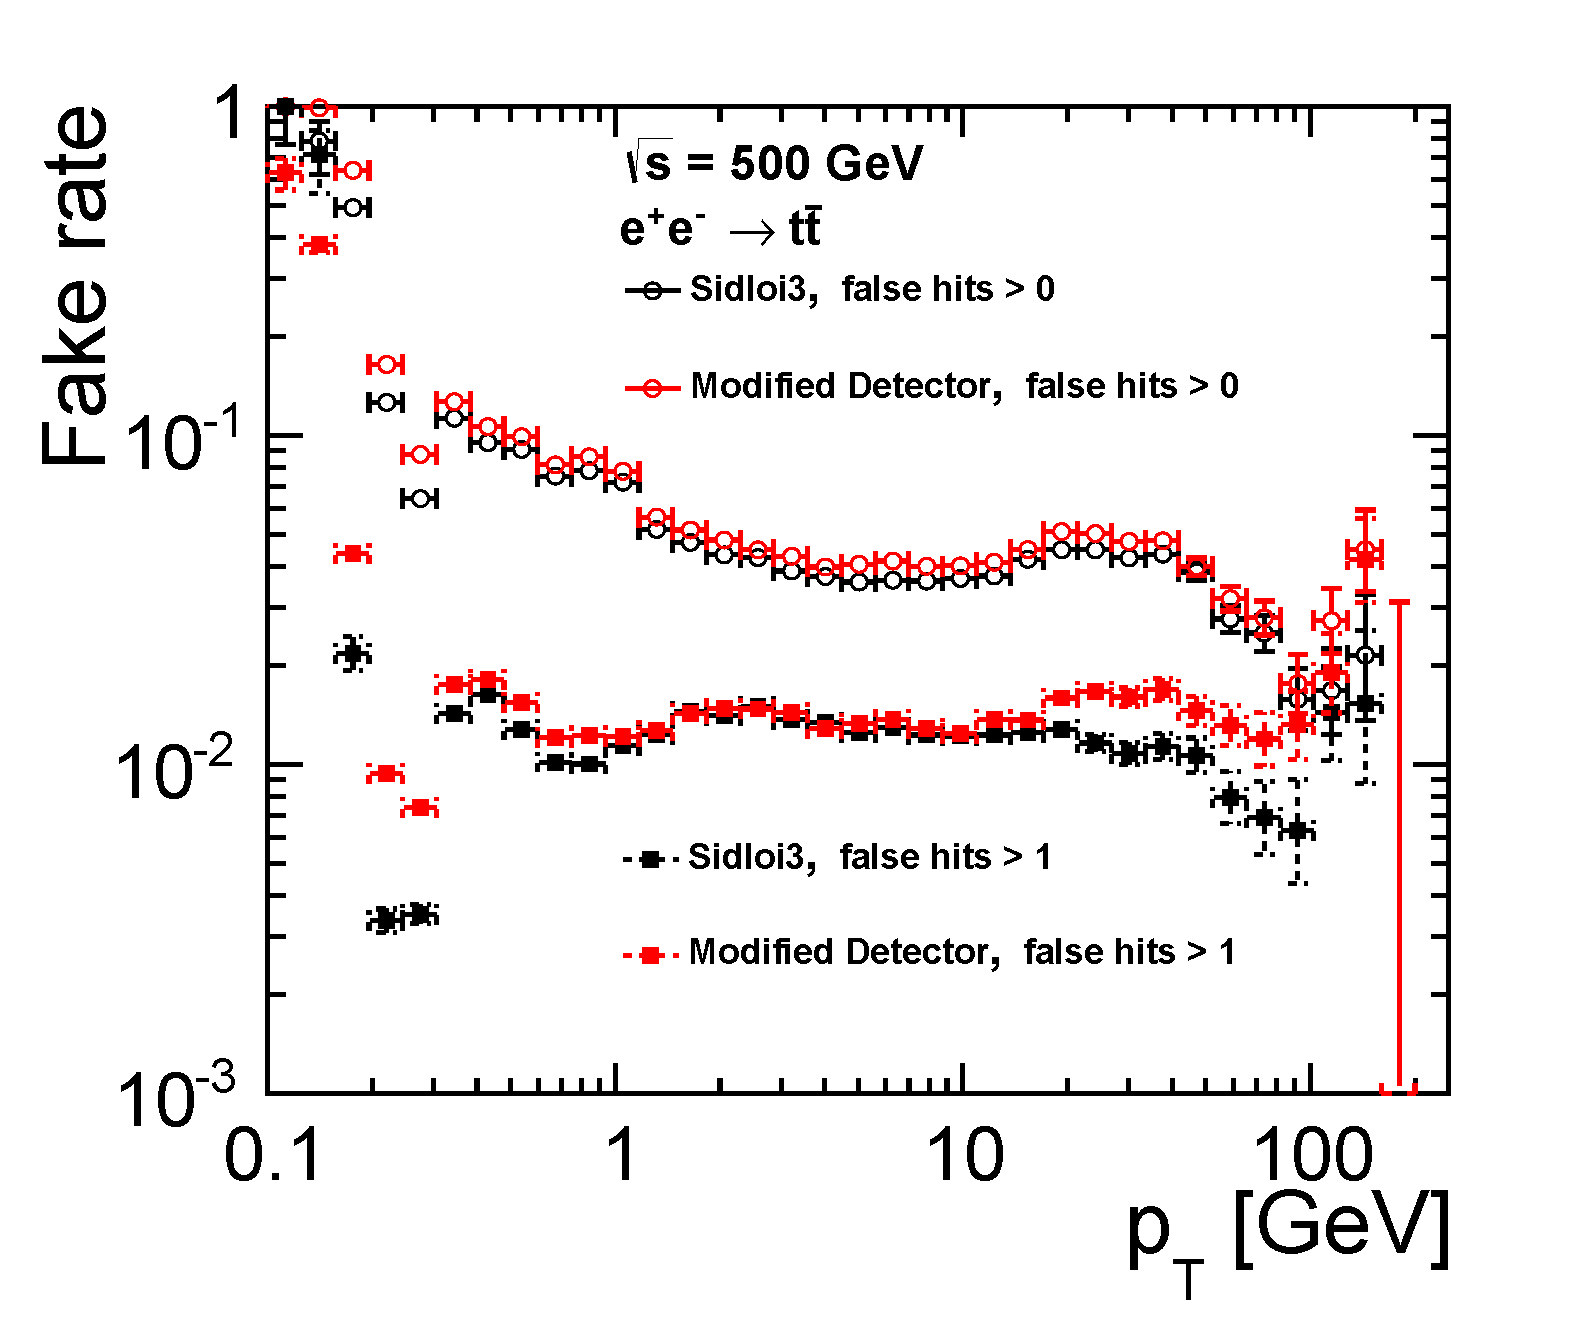
\includegraphics[width=3.0in]{eettbarFakeRatePt_sidloi3_det_vtxbar_3doublet.png}
\subcaption{Fake Rate vs.~$p_{T}$}\label{fig:eettbarfakeratept}
\end{minipage}
\caption{The fake rate of tracks for $\ee \rightarrow \ttbar$ at $ \sqrt{s} = $ 500 GeV as a function of (a) polar angle and
 (b) transverse momentum.}
\label{fig:eettbarfakerate}
\end{figure}
%% ttbb fake rate
\begin{figure}
\begin{minipage}{.5\textwidth}
\centering
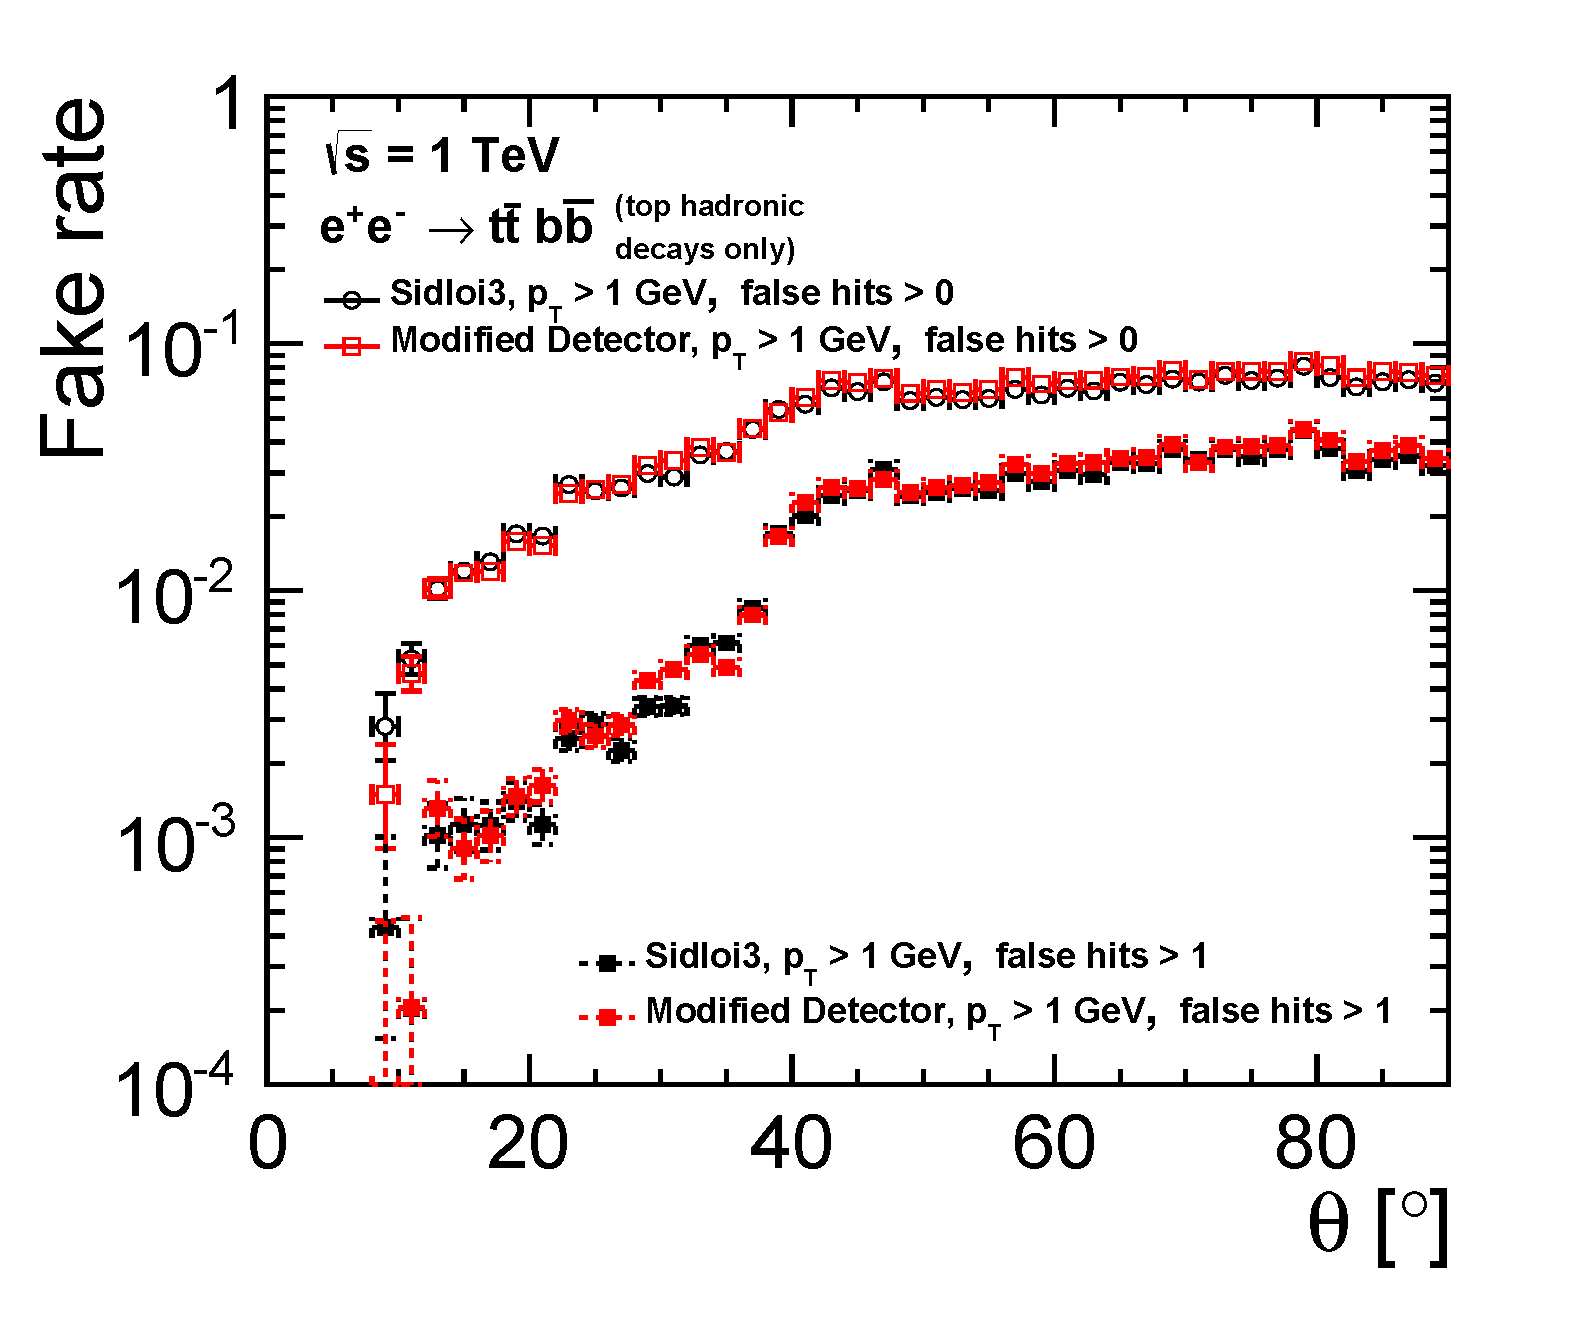
\includegraphics[width=3.0in]{ttbb6qallFakeRateTheta_sidloi3_det_vtxbar_3doublet.png}
\subcaption{Fake Rate vs.~$\theta$}\label{fig:ttbbfakeratetheta}
\end{minipage}
\begin{minipage}{.5\textwidth}
\centering
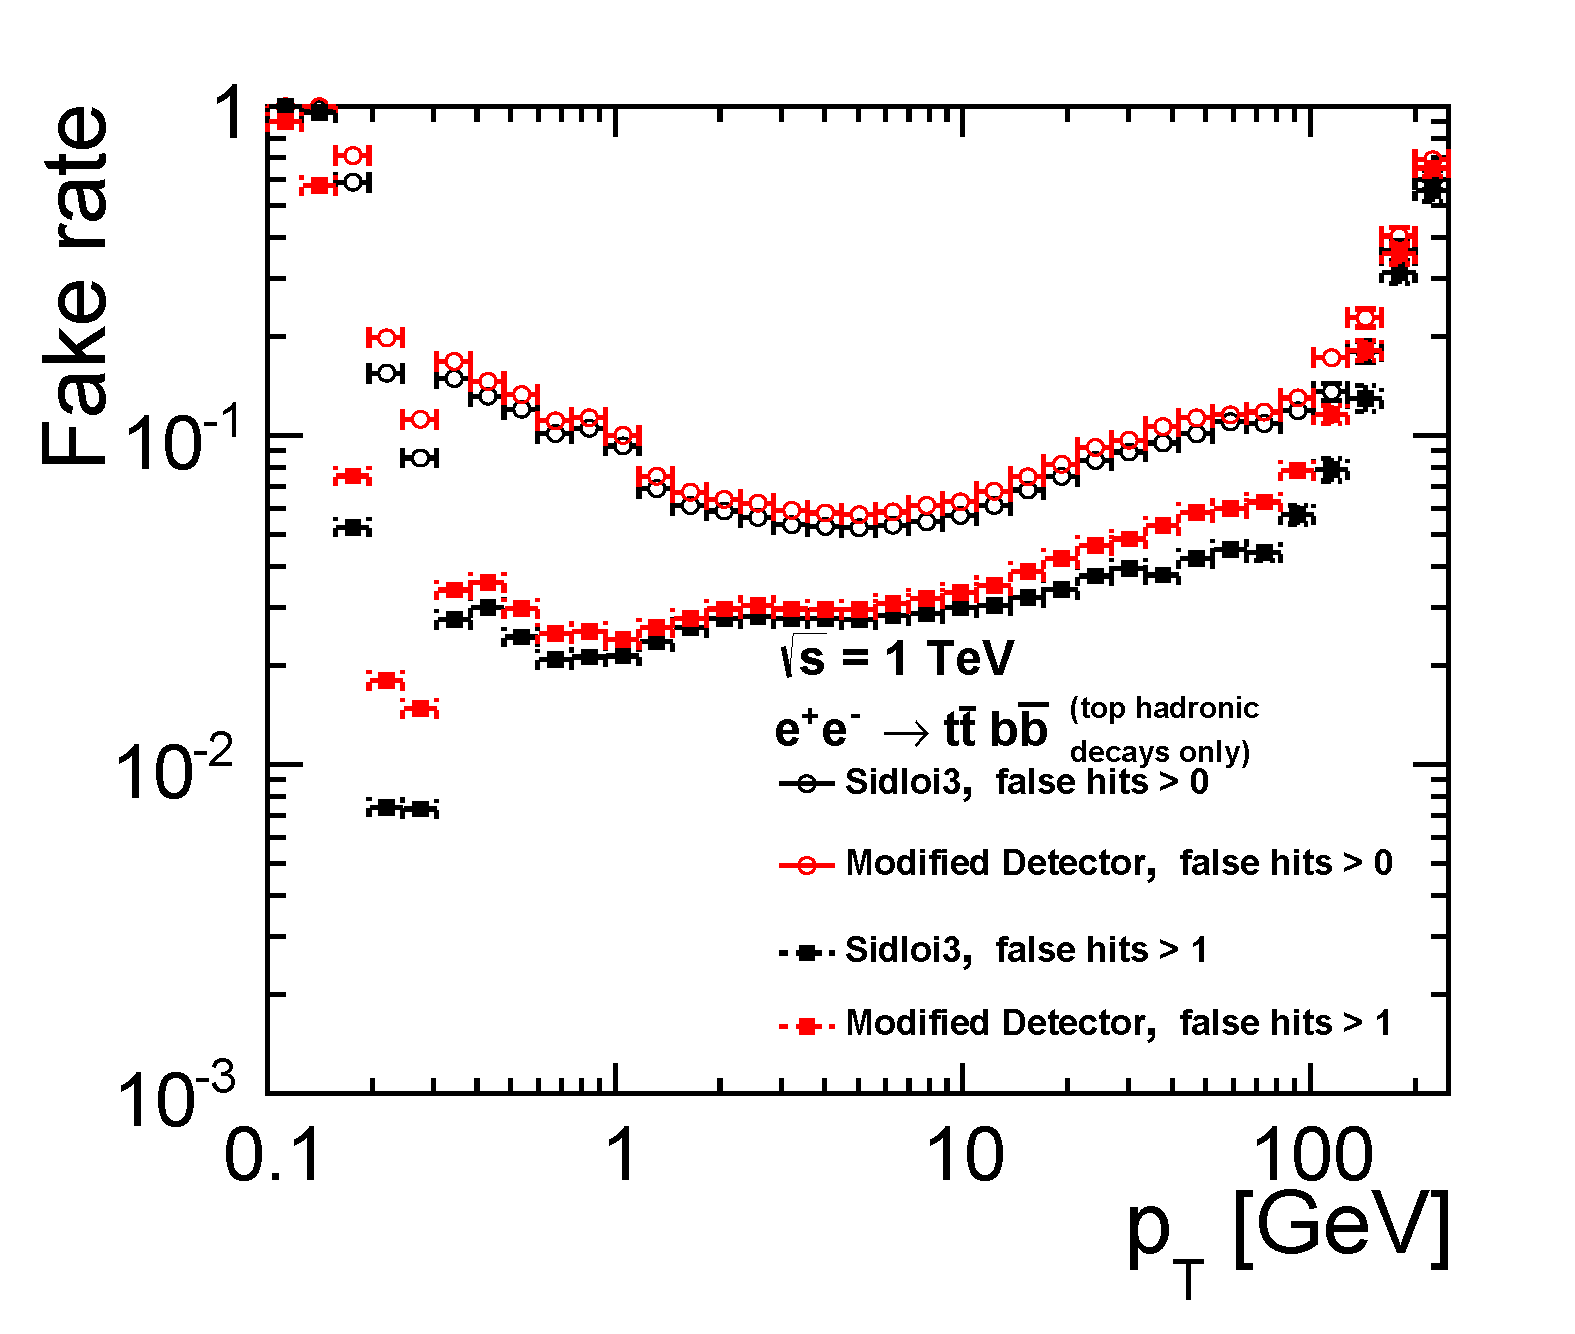
\includegraphics[width=3.0in]{ttbb6qallFakeRatePt_sidloi3_det_vtxbar_3doublet.png}
\subcaption{Fake Rate vs.~$p_{T}$}\label{fig:ttbbfakeratept}
\end{minipage}
\caption{The fake rate on tracks for $\ee \rightarrow \ttbar \bbbar$ at $ \sqrt{s} = $ 1 TeV as a function of (a) polar angle and
 (b) transverse momentum.}
\label{fig:ttbbfakerate}
\end{figure}

%\subsection{Tracking Resolution}
%\subsubsection{Impact Parameter Resolutions}
\subsection{Impact Parameter Resolutions}
\subsubsection{Single Muons}
For both detectors, the transverse impact parameter resolution improves as polar angle increases,
and is better for higher momenta (figure~\ref{fig:muond0restwodetectors}).
In particular, for muons with $p \geq 10 $ GeV, transverse impact parameter resolution $\sigma(d_{0})$ is better
than $10~\mu m$ for polar angles $\theta > 20^{\circ}$ for both detectors.
The transverse impact parameter resolution improves to $4~\mu m$ for $p \geq 10 $ GeV muons
at polar angles $\theta > 50^{\circ}$ for both detectors.
Muons with $p =  1$ GeV achieve transverse impact parameter resolution slightly greater than
$10 \mu m$ at $\theta =  90^{\circ}$.
For lower polar angles ($\theta < 90^{\circ}$), the resolution worsens as with $p = $ 10 GeV and 100 GeV muons.

$Z$-axis impact parameter resolution $\sigma(z_{0})$ (figure~\ref{fig:muonz0restwodetectors}) also improves as polar angle increases
and in general shows a greater dependence on polar angle, for both detectors.
For low polar angles ($\theta \lessapprox 35^{\circ}$), $z$-axis impact parameter resolution
reaches values roughly an order of magnitude greater than transverse impact parameter resolution
 for $p = $ 1, 10, and 100 GeV muons.
However, as polar angle increases ($\theta > 40^{\circ}$), muons with $p = 1$ GeV demonstrate
$z$-axis impact parameter resolution $\sigma(z_{0})$ slightly greater than $10 \mu m$,
values nearly equal to the transverse impact parameter resolution for $p = 1$ GeV muons (figure~\ref{fig:muond0restwodetectors}).
As for $p = $ 10 and 100 GeV muons, though $z$-axis impact parameter resolution does not quite reach
as low as transverse impact parameter resolution for greater polar angles ($\theta > 40^{\circ}$), $\sigma(z_{0})$
nevertheless reaches microns resolution for both detectors.

The ratio of the performance of the modified detector to
the Sidloi3 benchmark,
\begin{equation}
%R=\frac{\sigma(X)_{\mbox{\scriptsize{Modified Detector}}}}{\sigma(X)_{\mbox{\scriptsize{Sidloi3}}}}, X = d_{0}\mbox{ or } z_{0},
R=\frac{X_{\mbox{\scriptsize{Modified Detector}}}}{X_{\mbox{\scriptsize{Sidloi3}}}}, X = \sigma(d_{0})\mbox{ or } \sigma(z_{0}),
\label{eq:impactparameter}
\end{equation}
is plotted in figure~\ref{fig:muond0resratio} for 
the transverse impact parameter resolution, $\sigma(d_{0})$,
and in figure~\ref{fig:muonz0resratio} for 
the $z$-axis impact parameter resolution, $\sigma(z_{0})$, for these momenta.
\begin{figure}[h!]
\begin{minipage}{3.8in}
\centering
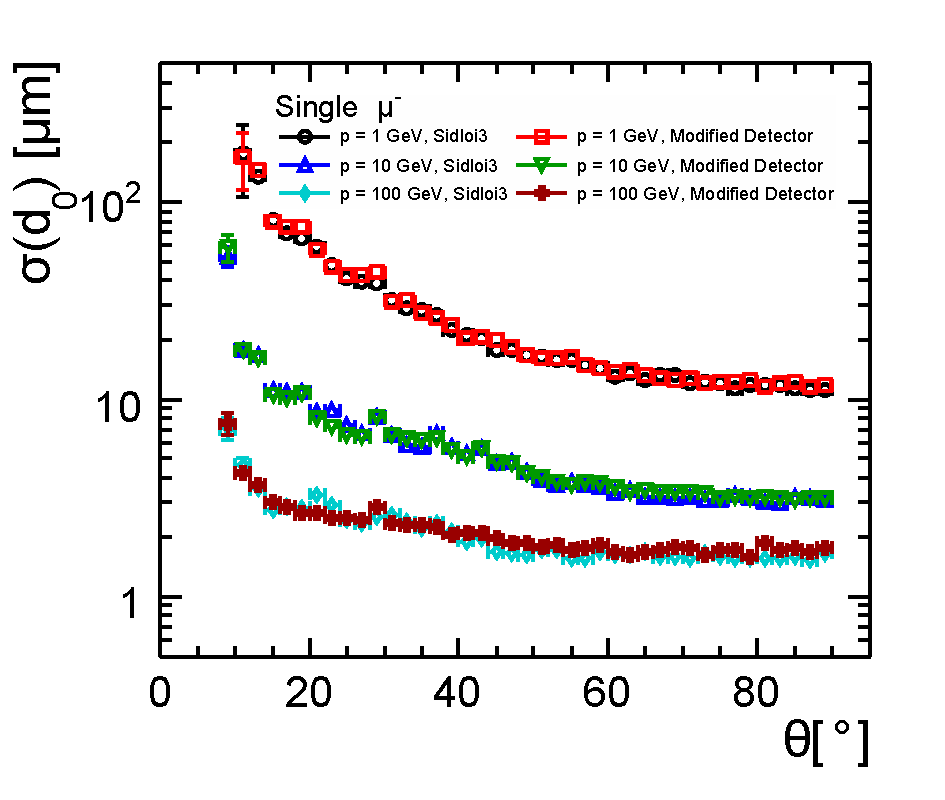
\includegraphics[width=3.8in]{muonD0ResolutionThetaTwoDetectors2.pdf}
\subcaption{$\sigma(d_{0})$ vs.~$\theta$, both detectors}\label{fig:muond0restwodetectors}
\end{minipage}
\begin{minipage}{2.0in}
\centering
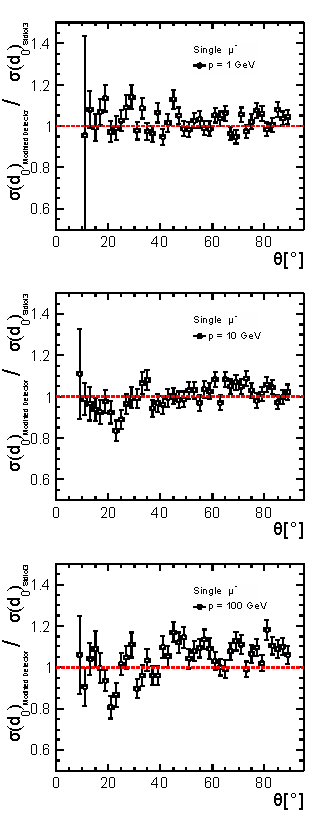
\includegraphics[width=2.0in]{muonD0ResRatio2.pdf}
%\subcaption{Ratio of transverse impact parameter resolutions}\label{fig:muond0resratio}
%\subcaption{$\sigma(d_{0})_{\mbox{\tiny{Mod.~Detector}}}/\sigma(d_{0})_{\mbox{\tiny{Sidloi3}}}$ vs.~$\theta$}\label{fig:muond0resratio}
\subcaption{$\sigma(d_{0})$ ratio vs.~$\theta$}\label{fig:muond0resratio}
\end{minipage}
\caption{(a) Transverse impact parameter resolution as a function of polar angle for single muons of various energies for both detectors.
(b) The ratio of the impact parameter resolutions as a function of polar angle.}
\label{fig:muond0res}
\end{figure}
%%% muon z0 resolution
\begin{figure}[h!]
\begin{minipage}{3.8in}
\centering
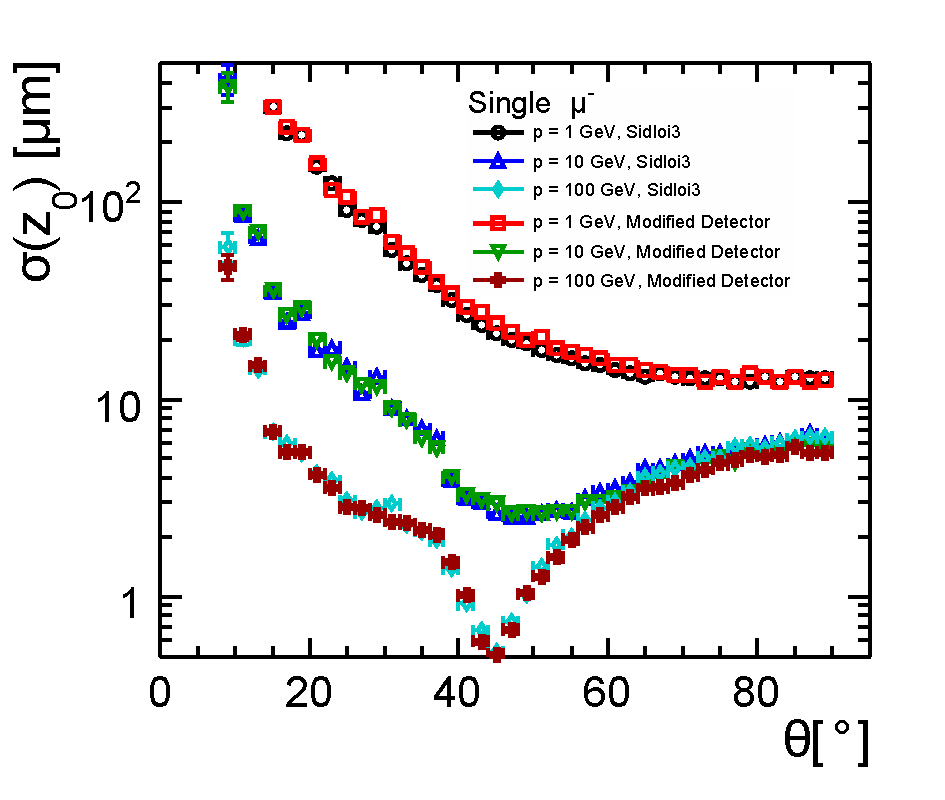
\includegraphics[width=3.8in]{muonZ0ResolutionThetaTwoDetectors2.pdf}
\subcaption{$\sigma(z_{0})$ vs.~$\theta$, both detectors}\label{fig:muonz0restwodetectors}
\end{minipage}
\begin{minipage}{2.0in}
\centering
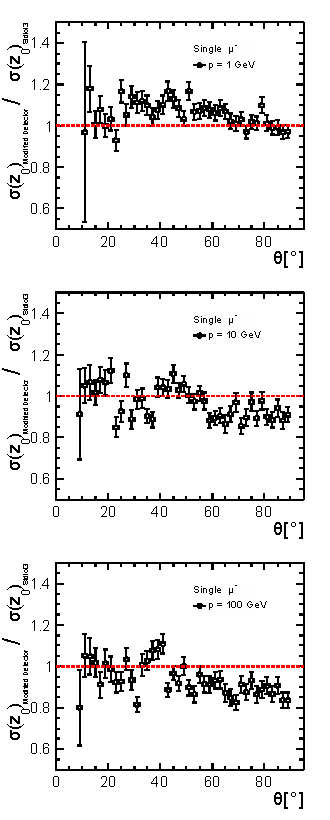
\includegraphics[width=2.0in]{muonZ0ResRatio2.pdf}
\subcaption{$\sigma(z_{0})$ ratio vs.~$\theta$}\label{fig:muonz0resratio}
\end{minipage}
\caption{(a) $Z$-axis impact parameter resolution as a function of polar angle for single muons of various energies for both detectors.
(b) The ratio of the impact parameter resolutions.}
\label{fig:muonz0res}
\end{figure}

Figure~\ref{fig:muonz0restwodetectors} shows the $z$-impact parameter
resolution for the two detector configurations.
The unusual dip in $z$-impact parameter resolution at
$\theta \approx 45^{\circ}$ for $p = $ 100 GeV muons% (figure~\ref{fig:muonz0restwodetectors})
is due to the fact that the polar angle reconstruction does not use the outer tracker barrel hits, instead using only the
vertex detector hits and the outer tracker disks.
This results in a large increase in lever arm just before the barrel region ends (figure~\ref{fig:coverage}),
which results in a rapid improvement of the $z$ impact parameter resolution.
As the lever arm continues to shorten as the polar angle increases ($\theta > 45^{\circ}$),
the resolution starts worsening.
%Nearly identical results for $\sigma(z_{0})$ are demonstrated and briefly explained for Sidloi3 in the SiD DBD~\cite{Behnke:2013lya}.
%%% muon d0 resolution

As figure~\ref{fig:muond0resratio} indicates, the transverse impact parameter resolution of the modified detector
is usually worse for $p =$ 100 GeV
at $\theta > 45^{\circ}$
%except at $\theta \approx 65^{\circ}$ and $\theta \approx 75^{\circ}$, where both detectors perform equally.
for muons with $p = 100$ GeV.% at polar angles $\theta < 45^{\circ}$,
The modified detector performed better than %(at $ 20^{\circ} < \theta$) or as well
%as (at $30^{\circ} < \theta < 40^{\circ}$) 
Sidloi3 at $\theta > 20^{\circ}$.
For muons with $p = 10$ GeV, the modified detector performs better at lower polar angles ($\theta < 30^{\circ}$).
At higher polar angles ($\theta > 30^{\circ}$), both detectors perform equally to within the error bars.
%except at $\theta \approx 70^{\circ}$.
Finally, for muons with $p = 1$ GeV, both detectors performed equally to within error bars for a wide polar angle range ($10^{\circ} < \theta < 90^{\circ}$).
%except at occasional spots where the modified detector performs worse
%(for example, $\theta \approx 20^{\circ}, 35^{\circ}, 45^{\circ}, 85^{\circ}$).
In general, the modified detector tends to perform worse for higher polar angles and better for lower polar angles,
also for high momenta.
%and that too usually for higher momentum single muons. At lower momenta, the distinction in performance is less pronounced.

Figure~\ref{fig:muonz0resratio} shows the ratio of the $z$-impact parameter resolution 
for the two detector configurations. 
%behaves differently than transverse impact parameter resolution.
In general, the modified detector demonstrates improved $z$-impact parameter resolution for large polar angles at high momenta.
Specifically, for muons with $p = 100$ GeV, the modified detector has better $\sigma(z_{0})$ for $\theta > 45^{\circ}$.
For muons with $p = 10$ GeV, the polar angle range for improved $z$-axis parameter resolution falls to $\theta > 55^{\circ}$.
On the other hand, for $p = 1$ GeV muons, the modified detector performs worse than Sidloi3 for 
a wide polar angle ($25^{\circ} < \theta < 65^{\circ}$) and at no polar angle does performance
dip in the modified detector's favor outside of the error bars, except slightly at $\theta \approx 25^{\circ}$.

\subsubsection{$\ee \rightarrow \ttbar$, $ \sqrt{s} = $ 500 GeV}
Figure~\ref{fig:eettbard0res} shows the transverse impact parameter resolution for both detectors
with respect to polar angle for $\ee \rightarrow \ttbar$ events.% demonstrates a similar 
The trend  is as seen for single muons (figure~\ref{fig:muond0restwodetectors}).
The resolution improves as polar angle increases, to $\sigma(d_{0}) \approx 10 \mu m$.
%, except
%right at $\theta = 90^{\circ}$, where the resolution gets worse for both detectors, more so for the
%modified detector than for Sidloi3.
Furthermore, as figure~\ref{fig:eettbard0resratio} indicates, the performance
of both detectors is nearly equal for a wide polar angle ($\theta > 35^{\circ}$).
For $\theta < 35^{\circ}$, the modified detector performed slightly better than Sidloi3 for $20^{\circ} < \theta < 35^{\circ}$,
and then Sidloi3 performed better for the relatively narrow polar angle $15^{\circ} < \theta < 20^{\circ}$.
%%% eettbar d0 resolution
\begin{figure}[h!]
\begin{minipage}{3.0in}
\centering
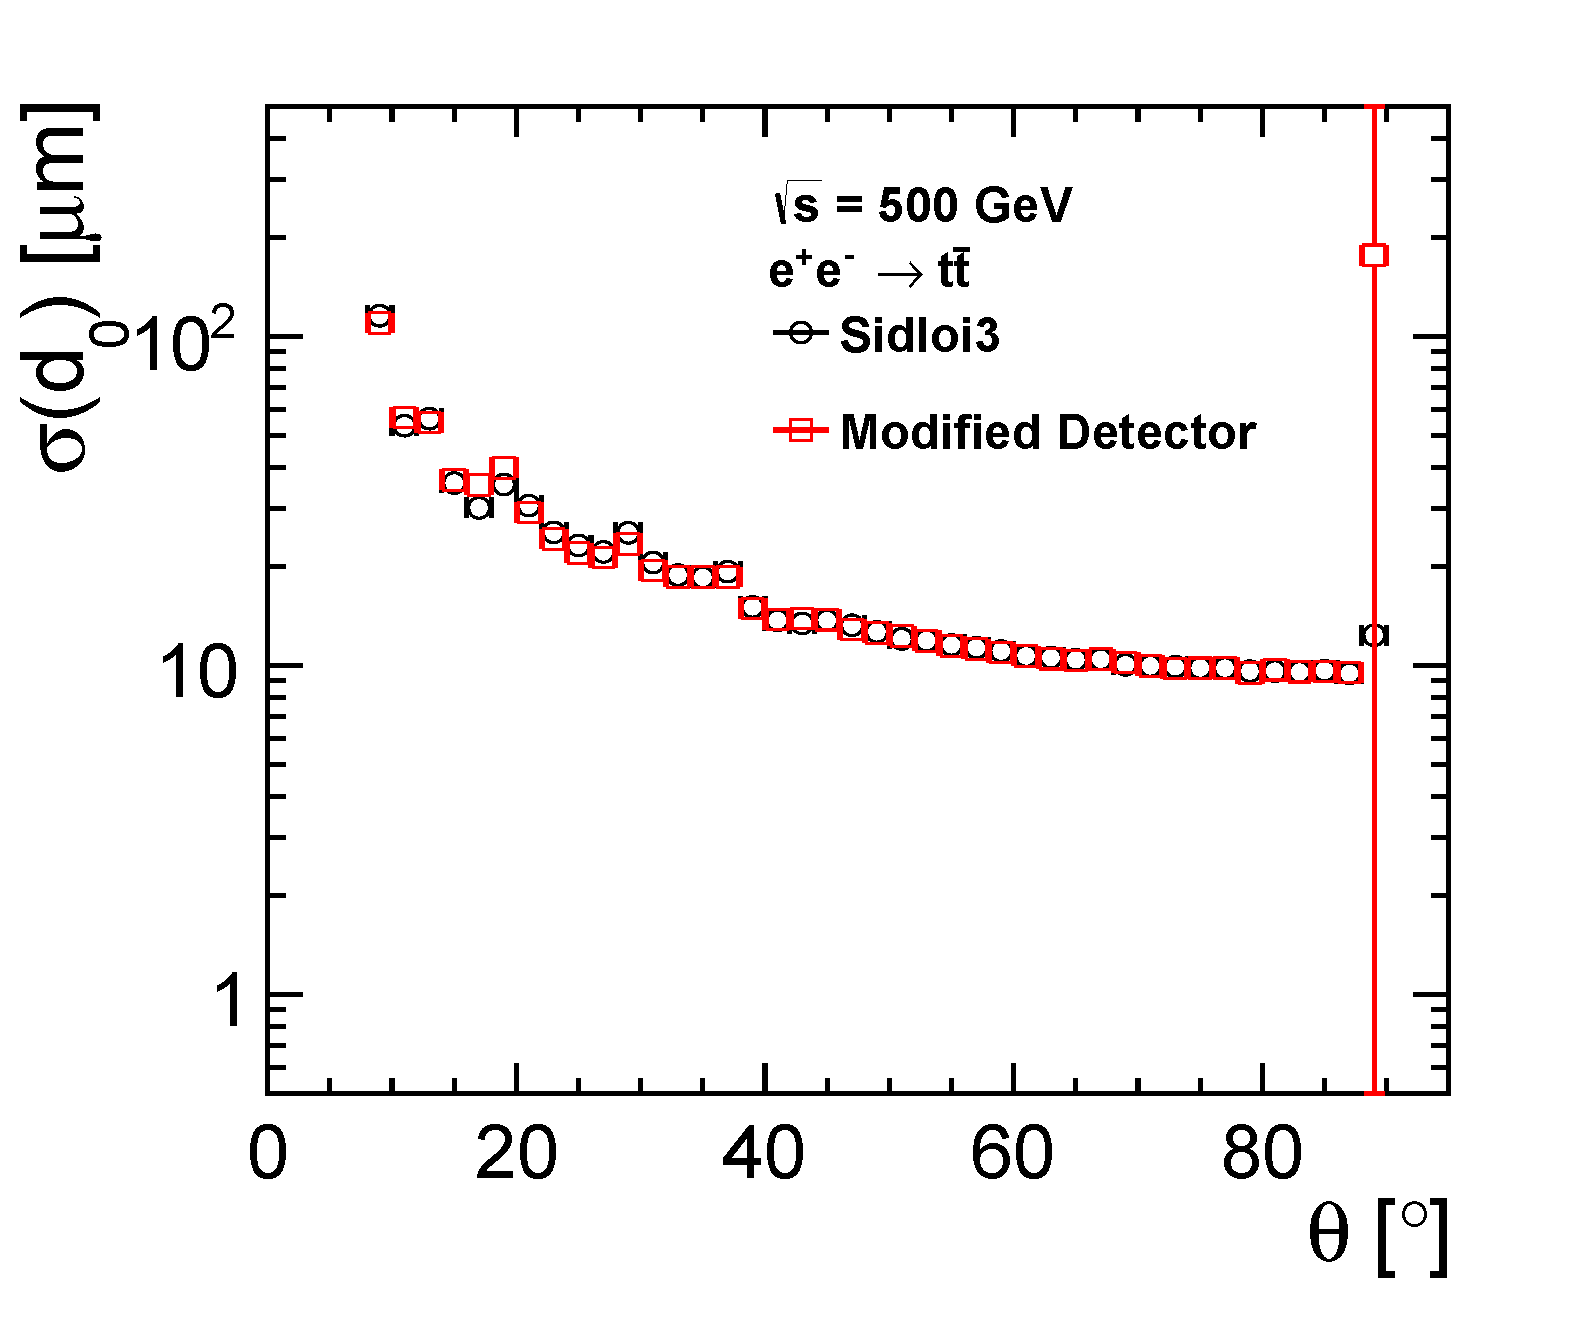
\includegraphics[width=2.9in]{eettbarD0ResolutionTheta_sidloi3_det_vtxbar_3doublet.png}
\subcaption{$\sigma(d_{0})$ vs.~$\theta$, both detectors}\label{fig:eettbard0restwodetectors}
\end{minipage}
\begin{minipage}{3.0in}
\centering
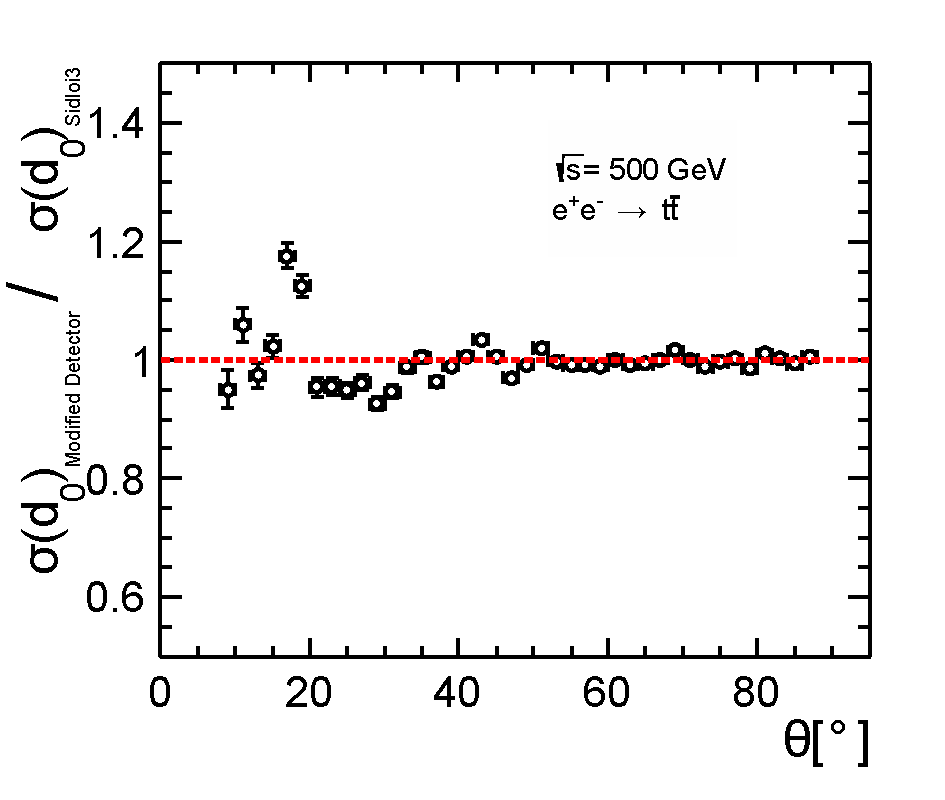
\includegraphics[width=3.0in]{eettbarD0ResolutionThetaRatio2.pdf}
\subcaption{$\sigma(d_{0})$ ratio vs.~$\theta$}\label{fig:eettbard0resratio}
\end{minipage}
\caption{(a) Transverse impact parameter resolution as a function of polar angle for
$\ee \rightarrow \ttbar$  at $\sqrt{s} = $ 500 GeV for both detector configurations.
(b) The ratio of the impact parameter resolutions as a function of polar angle.}
\label{fig:eettbard0res}
\end{figure}
%%% eettbar z0 resolution
\begin{figure}[h!]
\begin{minipage}{3.0in}
\centering
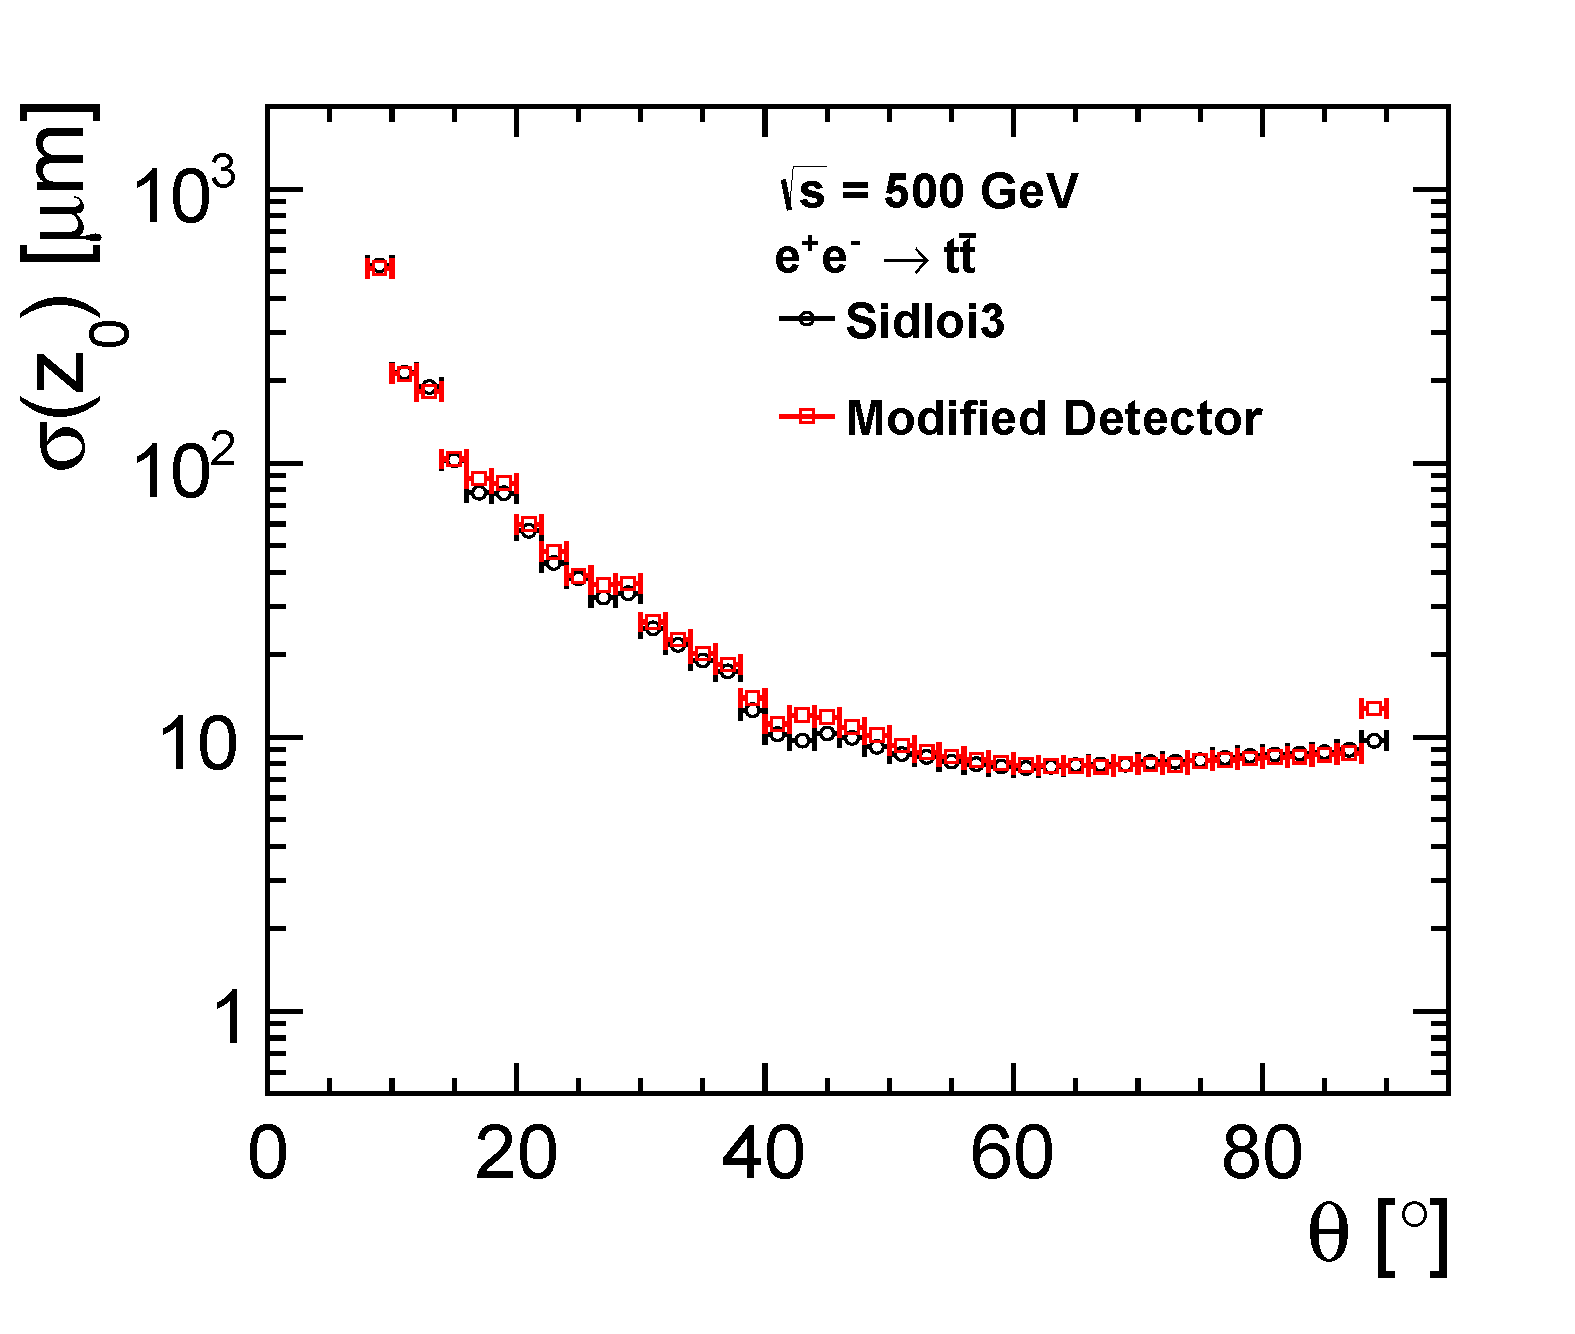
\includegraphics[width=3.0in]{eettbarZ0ResolutionTheta_sidloi3_det_vtxbar_3doublet.png}
\subcaption{$\sigma(z_{0})$ vs.~$\theta$, both detectors}\label{fig:eettbarz0restwodetectors}
\end{minipage}
\begin{minipage}{3.0in}
\centering
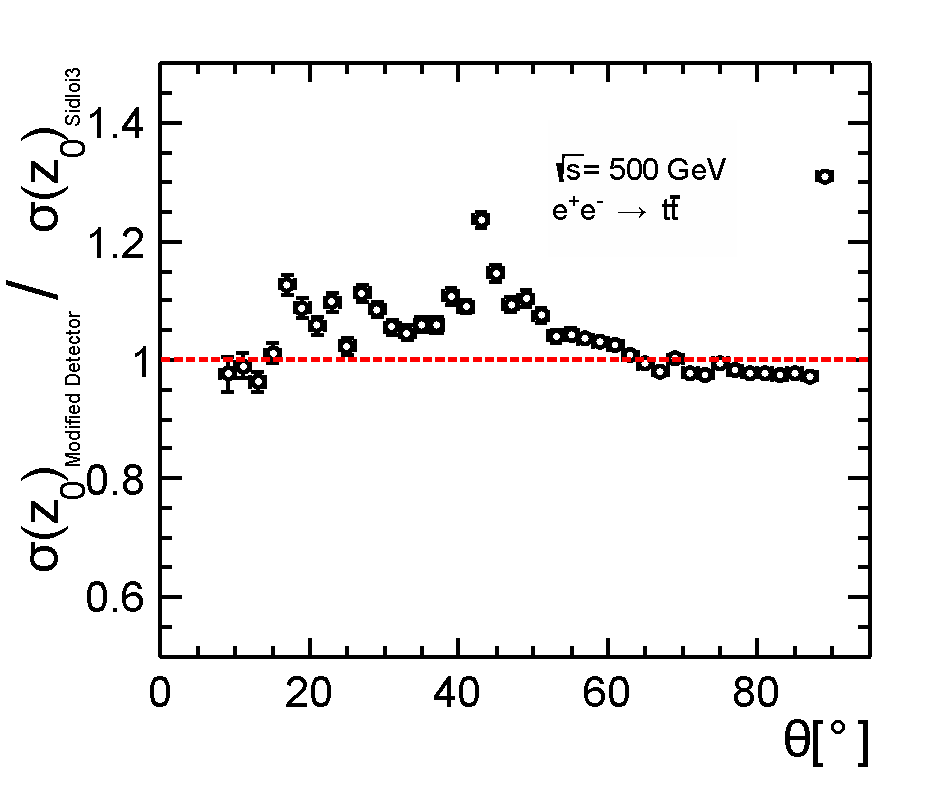
\includegraphics[width=3.0in]{eettbarZ0ResolutionThetaRatio2.pdf}
\subcaption{$\sigma(z_{0})$ ratio vs.~$\theta$}\label{fig:eettbarz0resratio}
\end{minipage}
\caption{(a) $Z$-axis impact parameter resolution as a function of polar angle for
$\ee \rightarrow \ttbar$  at $\sqrt{s} = $ 500 GeV for both detector configurations.
(b) The ratio of the impact parameter resolutions as a function of polar angle.}
\label{fig:eettbarz0res}
\end{figure}

The $z$-impact parameter resolution for $\ee \rightarrow \ttbar$ events (figure~\ref{fig:eettbarz0restwodetectors}) 
also behaved as it did for single muons (figure~\ref{fig:muonz0restwodetectors}).
The resolution reaches values $\approx 10 \mu m$ as polar angle increases ($\theta > 40^{\circ}$) for both detectors.
%As with transverse impact parameter resolution for $\ee \rightarrow \ttbar$ events,
There is a decrease
in $z$-axis impact parameter resolution right at $\theta = 90^{\circ}$ for both detectors, with the modified
detector demonstrating a greater increase. 
For lower polar angles ($\theta < 40^{\circ}$), $\sigma(z_{0})$ decreases to values roughly
an order of magnitude greater than transverse impact parameter resolution.
However, the two detectors do not have equal performance
with respect to $z$-impact parameter resolution, as figure~\ref{fig:eettbarz0resratio} demonstrates.
For a wide polar angle range ($20^{\circ} < \theta < 60^{\circ}$), the modified detector performs
worse than Sidloi3.
%Then, for $\theta > 70^{\circ}$, the modified detector performs slightly better.

\subsubsection{$\ee \rightarrow \ttbar \bbbar$ (hadronic decays only), $ \sqrt{s} = $ 1 TeV}
The $\ee \rightarrow \ttbar \bbbar$ events displayed similar performance as  the $\ee \rightarrow \ttbar$ events
 with respect to both transverse impact parameter resolution (figure~\ref{fig:ttbbd0res}) and 
$z$-impact parameter resolution (figure~\ref{fig:ttbbz0res}) for both detectors.
In particular, the transverse impact parameter resolution (figure~\ref{fig:ttbbd0res}) improved to $\sigma(d_{0}) \approx 10 \mu m$
as the polar angle increased and also saw a decrease right at $\theta =  90^{\circ}$ that was worse for
the modified detector than for Sidloi3.
Just as for the $\ee \rightarrow \ttbar$ events, 
the two detectors performed equally well for $\ee \rightarrow \ttbar \bbbar$ events
with respect to $\sigma(d_{0})$, albeit for a narrower polar angle range.
In particular, their performances were equal for $30^{\circ} < \theta < 70^{\circ}$.
For $\theta > 70^{\circ}$, the modified detector performed worse.
For $20^{\circ} < \theta < 30^{\circ}$, the modified detector performed slightly better.
%%% ttbb d0 resolution
\begin{figure}[h!]
\begin{minipage}{3.0in}
\centering
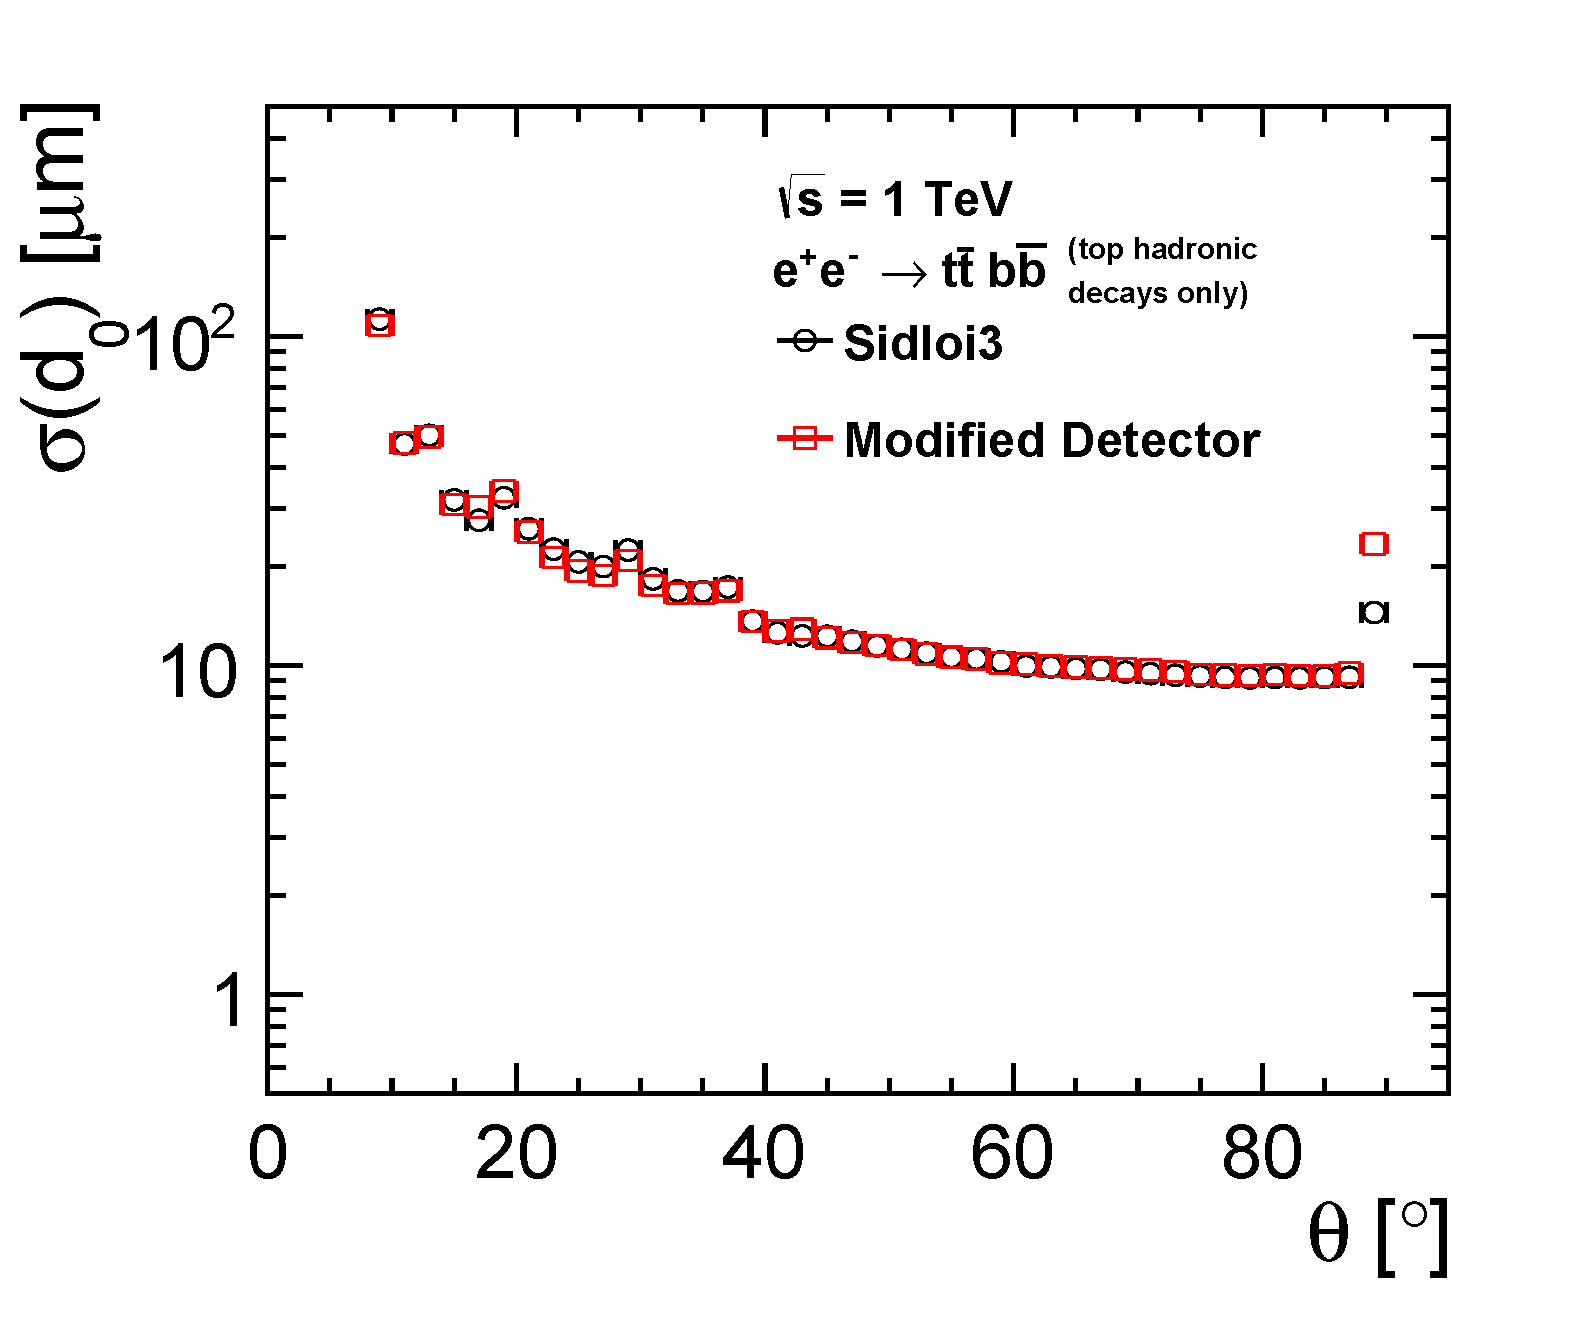
\includegraphics[width=3.0in]{ttbb6qallD0ResolutionTheta_sidloi3_det_vtxbar_3doublet.png}
\subcaption{$\sigma(d_{0})$ vs.~$\theta$, both detectors}\label{fig:ttbbd0restwodetectors}
\end{minipage}
\begin{minipage}{3.0in}
\centering
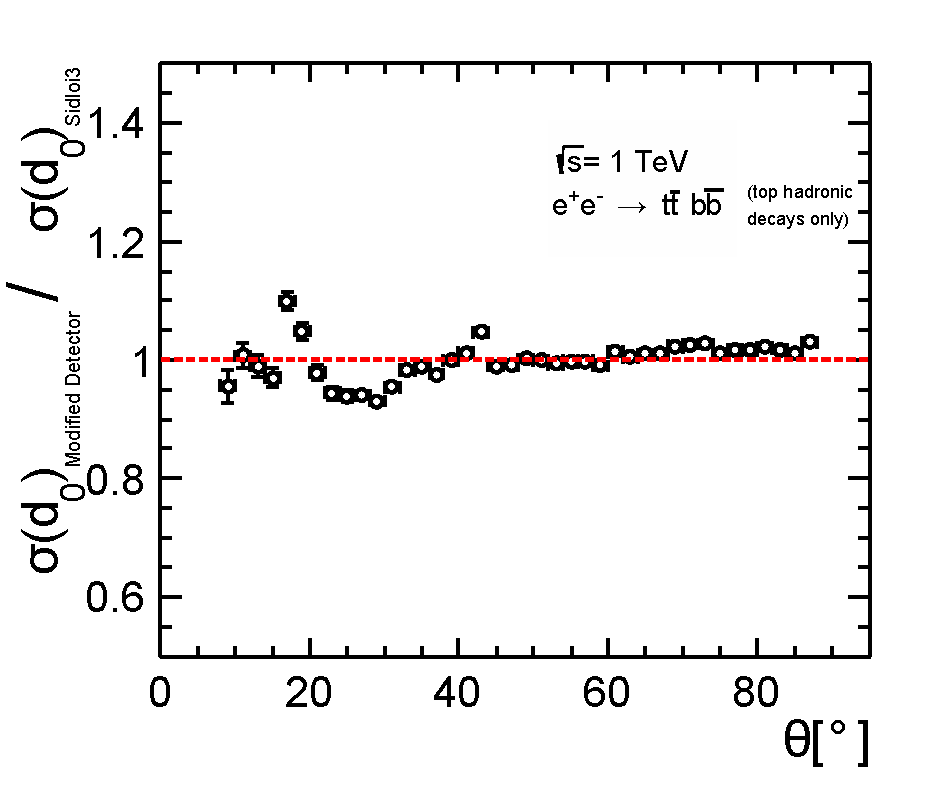
\includegraphics[width=3.0in]{ttbb6qallD0ResolutionThetaRatio2.pdf}
\subcaption{$\sigma(d_{0})$ ratio vs.~$\theta$}\label{fig:ttbbd0resratio}
\end{minipage}
\caption{(a) Transverse impact parameter resolution as a function of polar angle for
$\ee \rightarrow \ttbar \bbbar $  at $\sqrt{s} = $ 1 TeV for both detectors.
(b) The ratio of the impact parameter resolutions as a function of polar angle.}
\label{fig:ttbbd0res}
\end{figure}
%%% ttbb z0 resolution
\begin{figure}[h!]
\begin{minipage}{3.0in}
\centering
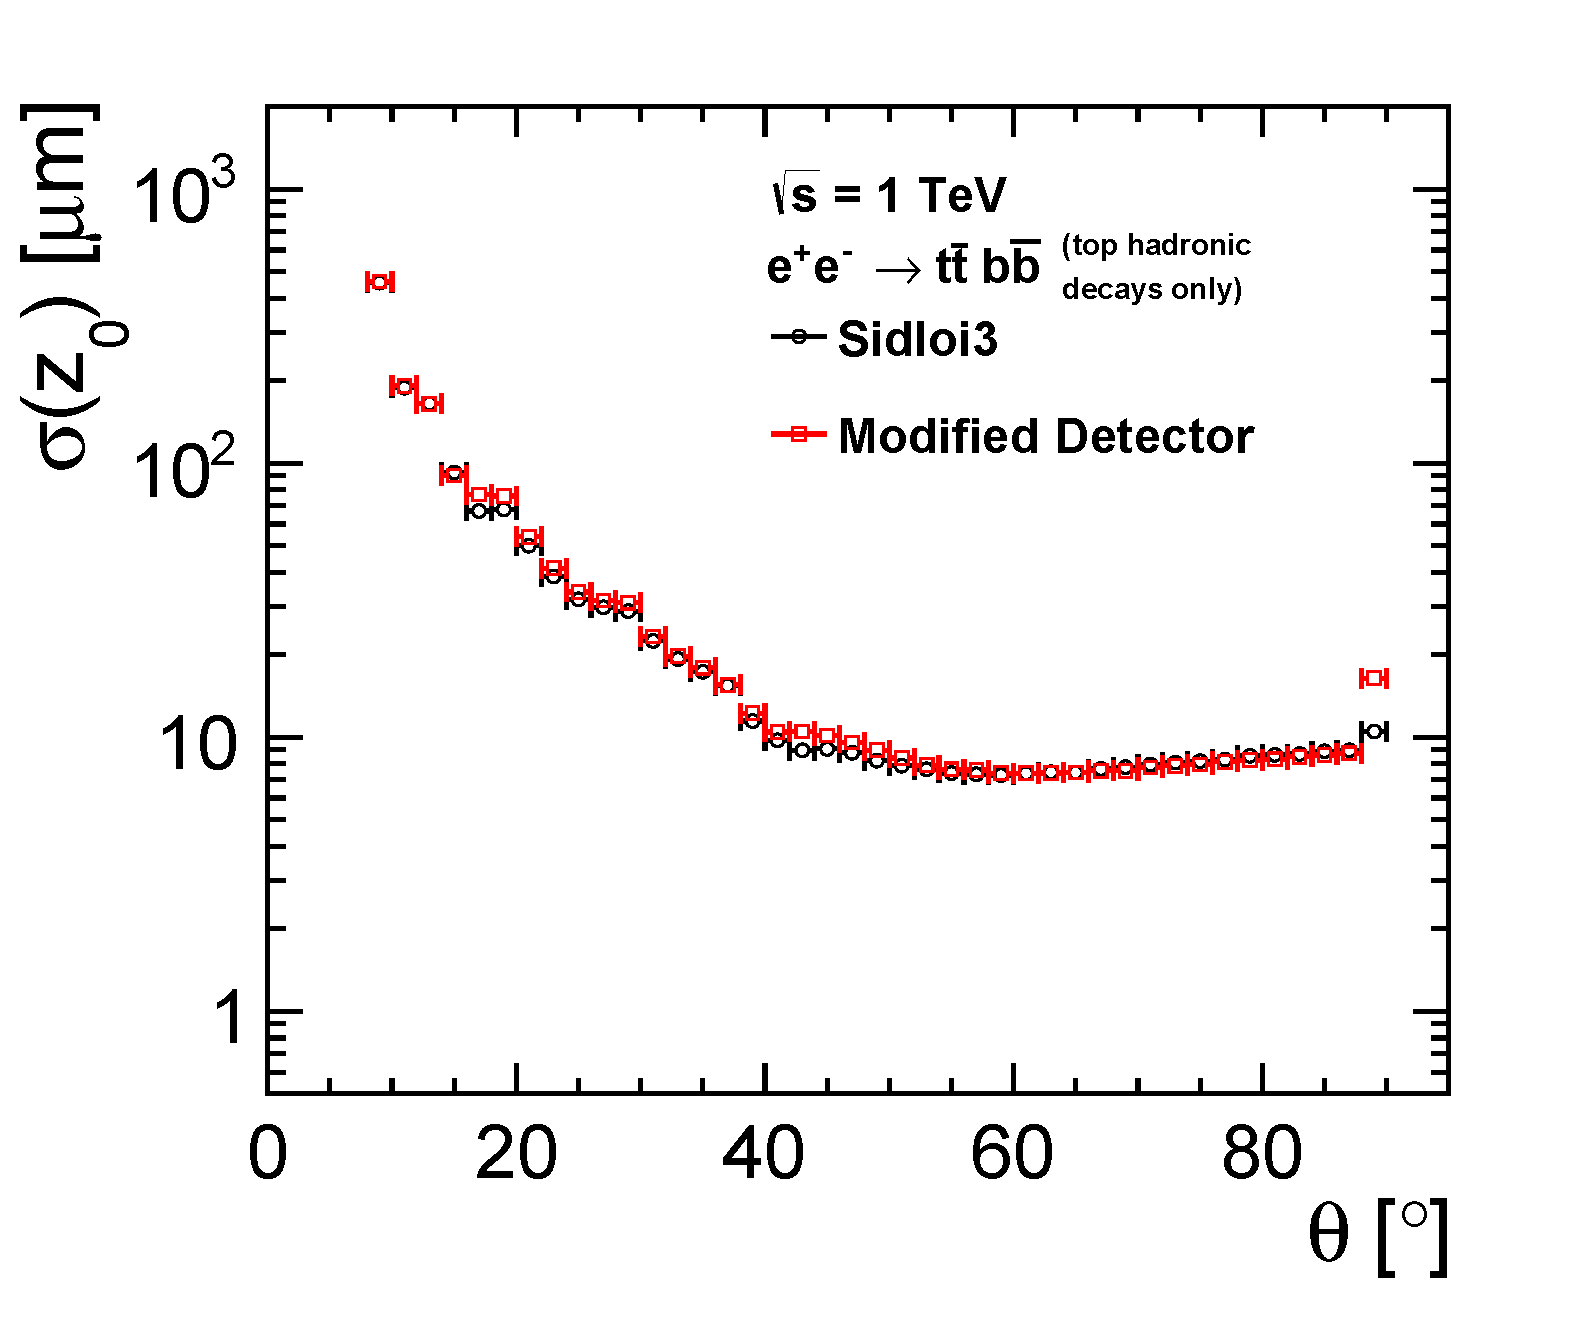
\includegraphics[width=3.0in]{ttbb6qallZ0ResolutionTheta_sidloi3_det_vtxbar_3doublet.png}
\subcaption{$\sigma(z_{0})$ vs.~$\theta$, both detectors}\label{fig:ttbbz0restwodetectors}
\end{minipage}
\begin{minipage}{3.0in}
\centering
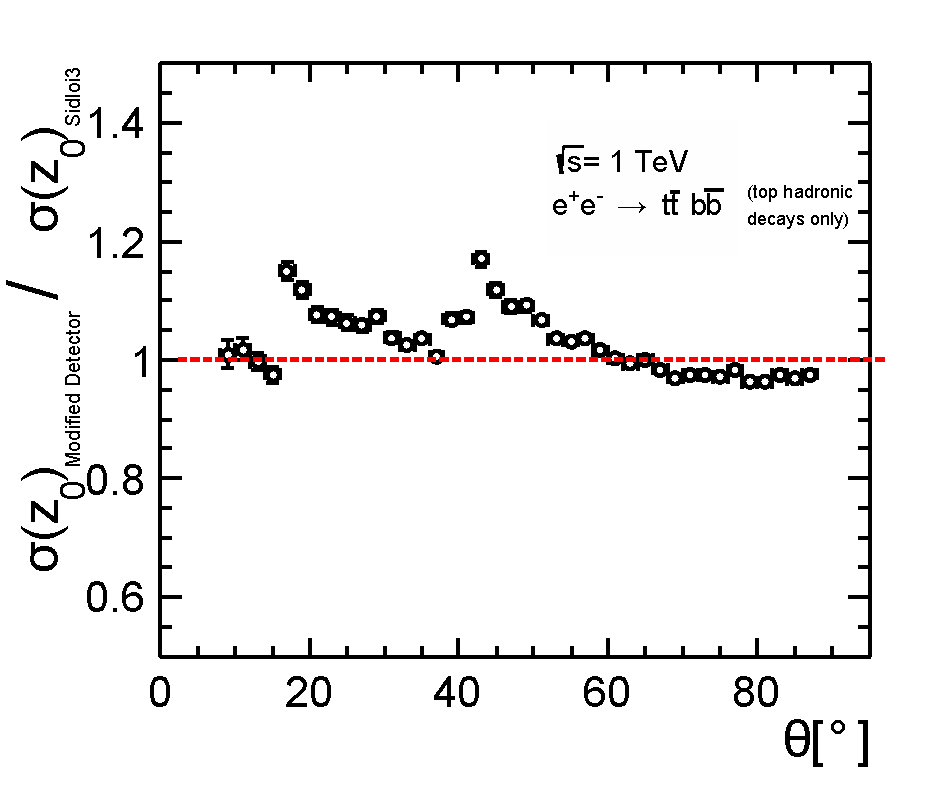
\includegraphics[width=3.0in]{ttbb6qallZ0ResolutionThetaRatio2.pdf}
\subcaption{$\sigma(z_{0})$ ratio vs.~$\theta$}\label{fig:ttbbz0resratio}
\end{minipage}
\caption{(a) $Z$-impact parameter resolution as a function of polar angle for
$\ee \rightarrow \ttbar \bbbar$  at $\sqrt{s} = $ 1 TeV for both detectors.
(b) The ratio of the impact parameter resolutions as a function of polar angle.}
\label{fig:ttbbz0res}
\end{figure}

The $z$-impact parameter resolution (figure~\ref{fig:ttbbz0res}), both detectors again reached $\approx 10 \mu m$
for greater polar angles ($\theta > 40^{\circ}$) and were almost an order of magnitude worse than for $\sigma(d_{0})$
at low polar angles ($\theta < 20^{\circ}$).
Just as with the $\ee \rightarrow \ttbar$ events, the ratio of the two detectors' $z$-axis impact
parameter resolutions unequivocally shows regions in which one detector performs better than the other.
As figure~\ref{fig:ttbbz0resratio} shows, the modified detector had slightly better $\sigma(z_{0})$ for $\theta > 65^{\circ}$.
The modified detector had worse $\sigma(z_{0})$ for $20^{\circ} < \theta < 65^{\circ}$.

\subsection{Transverse Momentum Resolution}
The transverse momentum resolution was fit according to the parameterization
\begin{equation}
\frac{\sigma(p_{T})}{p_{T}^{2}} = a \oplus \frac{b}{p\sin{\theta}},
\label{eq:pt}
\end{equation}
where $\oplus$ denotes addition in quadrature. 
As figure~\ref{fig:ptres} illustrates, both detectors achieve a transverse momentum resolution $\sigma(p_{T})/p_{T}^{2} < 10^{-4}$ 
for $\theta > 30^{\circ}$ for high momentum ($p > 100$  GeV) tracks.
%as was also demonstrated in~\cite{Behnke:2013lya}.
For $\theta = 90^{\circ}$, both detectors achieve  $\sigma(p_{T})/p_{T}^{2} < 10^{-5}$ for tracks with $p \gtrapprox 200$ GeV.
%again consistent with the results presented in~\cite{Behnke:2013lya}.
%The coefficients for the fit to equation~\ref{eq:pt} are printed in the plots in figure~\ref{fig:ptres} and have
%similar values for both detectors.
%The results indicate comparable transverse momentum resolution for both detectors.
The transverse momentum resolution is comparable for both detectors.
%%% muon pt res
\begin{figure}[h!]
\begin{minipage}{.5\textwidth}
\centering
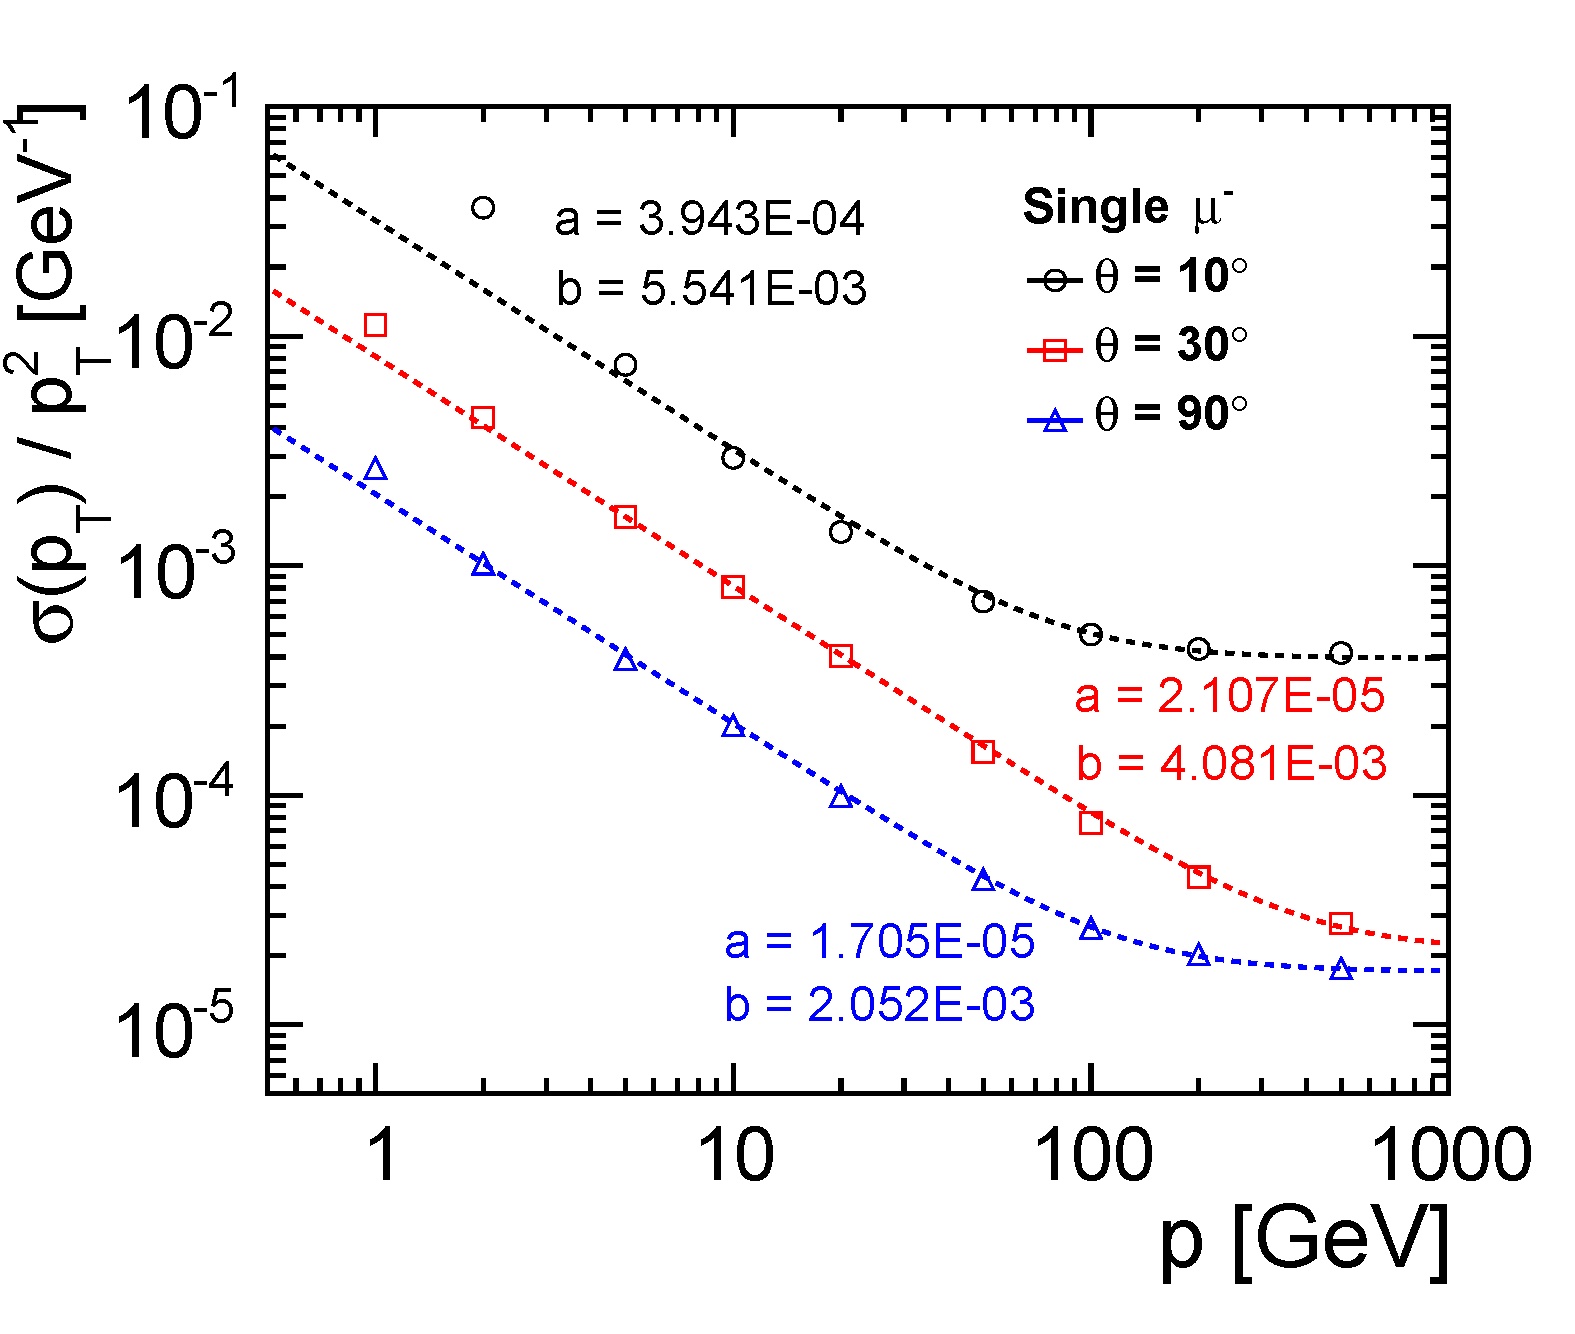
\includegraphics[width=3.0in]{sidloi3_muonPt2ResolutionP.png}
\subcaption{Sidloi3}\label{fig:sidloi3ptres}
\end{minipage}
\begin{minipage}{.5\textwidth}
\centering
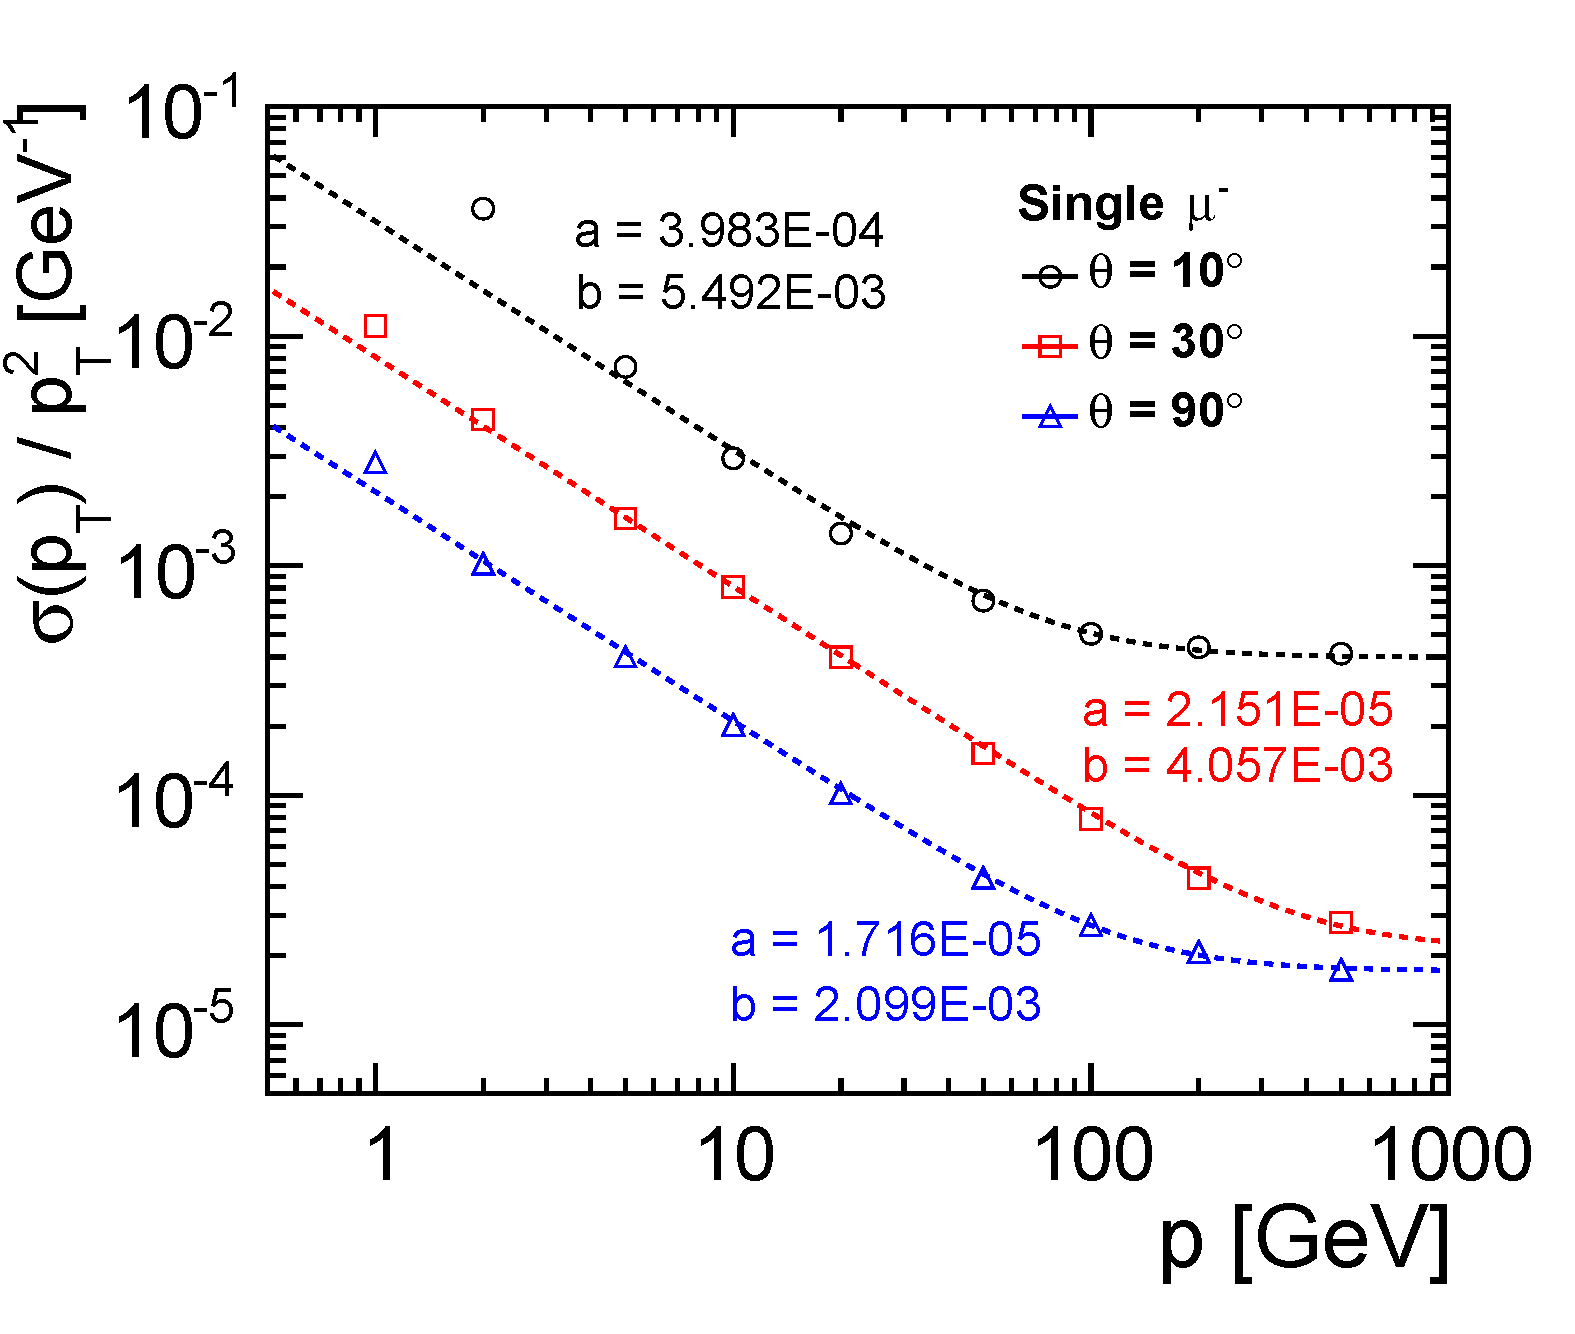
\includegraphics[width=3.0in]{det_vtxbar_3doublet_muonPt2ResolutionP.png}
\subcaption{Modified Detector}\label{fig:det_vtxbar_3doubletptres}
\end{minipage}
\caption{Transverse momentum resolution for single muons as a function of momentum for (a) Sidloi3 and (b) the modified detector.}
\label{fig:ptres}
\end{figure}

